%============================================================================%
% Antoine Géré (gereantoine@gmail.com).
% Ph.D. thesis. (2013--2015)
% (TITLE) %%TODO TITLE
% --
% Università degli Studi di Genova.
% http://www.unige.it
% --
% Dipartimento di Matematica,
% Via Dodecaneso 35, 16146 Genova, Italia.
%============================================================================%
% LaTeX environment, Kile : available at http://kile.sourceforge.net/
% --
% Package : available at http://www.ctan.org/
% --
% The comprehensive latex symbole list : available at http://www.ctan.org/tex-archive/info/symbols/comprehensive/
% Detexif (an attempt to simplify the search in the latex symbole list) : available at http://detexify.kirelabs.org/classify.html
% --
% Bibliography with Zotero : available at http://www.zotero.org/
% Bibtex style ????? 
% --
% Latex font catalogue : available at http://www.tug.dk/FontCatalogue/
%============================================================================%


\documentclass[12pt]{book}


%----------------------------------------------------------------------------%


%a
\usepackage{amscd}
\usepackage{amsmath}
\usepackage{amsfonts}
\usepackage{amssymb}
\usepackage{amsxtra}
\usepackage{array} 
%b
\usepackage[english]{babel}
%c
\usepackage{calligra}
\usepackage{cite}
\usepackage{color}
%e
\usepackage{enumitem}
%f
\usepackage{fancyhdr}
\usepackage{filecontents}
\usepackage[T1]{fontenc}
%g
\usepackage{geometry}
%h
\usepackage{hyperref}
%i
\usepackage[totoc]{idxlayout}
\usepackage[utf8]{inputenc}
%m
\usepackage{makeidx}
%n
\usepackage[amsmath,amsthm,thmmarks]{ntheorem}
%p
\usepackage{palatino}
%t
\usepackage{tikz}
%u
\usepackage{upgreek}
%w
\usepackage{wrapfig}


%----------------------------------------------------------------------------%


%\usepackage{cmbright}
%\usepackage[math]{iwona}
%\usepackage[light,condensed,math]{kurier}
%\usepackage[sfdefault]{quattrocento}


%----------------------------------------------------------------------------%


%\begin{filecontents}{biblio.bib}


%


%\end{filecontents}


%----------------------------------------------------------------------------%


\geometry{
a4paper,
left=27mm,
right=27mm,
top=24mm,
bottom=24mm,
}


%----------------------------------------------------------------------------%


\abovedisplayskip=12pt plus 3pt minus 9pt
\abovedisplayshortskip=0pt plus 3pt
\belowdisplayskip=12pt plus 3pt minus 9pt
\belowdisplayshortskip=7pt plus 3pt minus 4pt

 
%----------------------------------------------------------------------------%


\setcounter{tocdepth}{8}  
\setcounter{secnumdepth}{8}
\setlength\parindent{8pt}
\pdfoptionpdfminorversion=6


%----------------------------------------------------------------------------%


\renewcommand{\headrulewidth}{0pt}
\renewcommand{\footrulewidth}{0pt}


\setlength{\headheight}{22pt} 


\pagestyle{fancy}


\renewcommand{\chaptermark}[1]{ \markboth{#1}{} }
\renewcommand{\sectionmark}[1]{ \markright{#1} }


\fancyhf{}
\fancyhead[LE,RO]{\thepage}
\fancyhead[RE,CE]{}
\fancyhead[LO,CO]{}

\fancypagestyle{plain}{%
\fancyhf{}
}%


\DeclareMathAlphabet{\mathcalligra}{T1}{calligra}{m}{n}


%----------------------------------------------------------------------------%


\makeindex


%----------------------------------------------------------------------------%


\newcommand{\supp}{\mathsf{supp}}
\newcommand{\singsupp}{\mathsf{singsupp}}
\newcommand{\WF}{\mathsf{WF}}
\newcommand{\id}{\mathsf{id}}
\newcommand{\loc}{\mathsf{loc}}
\newcommand{\reg}{\mathsf{reg}}
\newcommand{\pp}{\mathsf{pp}}
\newcommand{\ms}{\mathsf{ms}}
\newcommand{\sd}{\mathsf{sd}}
\newcommand{\vol}{\mathsf{vol}}
\newcommand{\tr}{\mathsf{tr}}
\renewcommand{\Re}{\mathsf{Re}}
\newcommand{\MS}{\textbf{MS}}


\newcommand{\abs}[1]{\left|#1\right|}
\newcommand{\norm}[1]{\left|\left|#1\right|\right|}
\newcommand{\sm}[1]{\left\langle#1\right\rangle}
\newcommand{\wick}[1]{:\!{#1}\!:}


\renewcommand{\det}{\mathsf{det}}
\renewcommand{\sup}{\mathsf{sup}}
\renewcommand{\inf}{\mathsf{inf}}


\let\int\int
\def\bigint{\displaystyle\int}


%----------------------------------------------------------------------------%


\newcommand{\Acal}{\mathcal{A}}
\newcommand{\Bcal}{\mathcal{B}}
\newcommand{\Ccal}{\mathcal{C}}
\newcommand{\Dcal}{\mathcal{D}}
\newcommand{\Ecal}{\mathcal{E}}
\newcommand{\Fcal}{\mathcal{F}}
\newcommand{\Gcal}{\mathcal{G}}
\newcommand{\Hcal}{\mathcal{H}}
\newcommand{\Ical}{\mathcal{I}}
\newcommand{\Jcal}{\mathcal{J}}
\newcommand{\Kcal}{\mathcal{K}}
\newcommand{\Lcal}{\mathcal{L}}
\newcommand{\Mcal}{\mathcal{M}}
\newcommand{\Ncal}{\mathcal{N}}
\newcommand{\Ocal}{\mathcal{O}}
\newcommand{\Pcal}{\mathcal{P}}
\newcommand{\Qcal}{\mathcal{Q}}
\newcommand{\Rcal}{\mathcal{R}}
\newcommand{\Scal}{\mathcal{S}}
\newcommand{\Tcal}{\mathcal{T}}
\newcommand{\Ucal}{\mathcal{U}}
\newcommand{\Vcal}{\mathcal{V}}
\newcommand{\Wcal}{\mathcal{W}}
\newcommand{\Xcal}{\mathcal{X}}
\newcommand{\Ycal}{\mathcal{Y}}
\newcommand{\Zcal}{\mathcal{Z}}


%----------------------------------------------------------------------------%


\newcommand{\Abb}{\mathbb{A}}
\renewcommand{\Bbb}{\mathbb{B}}
\newcommand{\Cbb}{\mathbb{C}}
\newcommand{\Dbb}{\mathbb{D}}
\newcommand{\Ebb}{\mathbb{E}}
\newcommand{\Fbb}{\mathbb{F}}
\newcommand{\Gbb}{\mathbb{G}}
\newcommand{\Hbb}{\mathbb{H}}
\newcommand{\Ibb}{\mathbb{I}}
\newcommand{\Jbb}{\mathbb{J}}
\newcommand{\Kbb}{\mathbb{K}}
\newcommand{\Lbb}{\mathbb{L}}
\newcommand{\Mbb}{\mathbb{M}}
\newcommand{\Nbb}{\mathbb{N}}
\newcommand{\Obb}{\mathbb{O}}
\newcommand{\Pbb}{\mathbb{P}}
\newcommand{\Qbb}{\mathbb{Q}}
\newcommand{\Rbb}{\mathbb{R}}
\newcommand{\Sbb}{\mathbb{S}}
\newcommand{\Tbb}{\mathbb{T}}
\newcommand{\Ubb}{\mathbb{U}}
\newcommand{\Vbb}{\mathbb{V}}
\newcommand{\Wbb}{\mathbb{W}}
\newcommand{\Xbb}{\mathbb{X}}
\newcommand{\Ybb}{\mathbb{Y}}
\newcommand{\Zbb}{\mathbb{Z}}


%----------------------------------------------------------------------------%


\newcommand{\Arak}{\mathfrak{A}}
\newcommand{\Brak}{\mathfrak{B}}
\newcommand{\Crak}{\mathfrak{C}}
\newcommand{\Drak}{\mathfrak{D}}
\newcommand{\Erak}{\mathfrak{E}}
\newcommand{\Frak}{\mathfrak{F}}
\newcommand{\Grak}{\mathfrak{G}}
\newcommand{\Hrak}{\mathfrak{H}}
\newcommand{\Irak}{\mathfrak{I}}
\newcommand{\Jrak}{\mathfrak{J}}
\newcommand{\Krak}{\mathfrak{K}}
\newcommand{\Lrak}{\mathfrak{L}}
\newcommand{\Mrak}{\mathfrak{M}}
\newcommand{\Nrak}{\mathfrak{N}}
\newcommand{\Orak}{\mathfrak{O}}
\newcommand{\Prak}{\mathfrak{P}}
\newcommand{\Qrak}{\mathfrak{Q}}
\newcommand{\Rrak}{\mathfrak{R}}
\newcommand{\Srak}{\mathfrak{S}}
\newcommand{\Trak}{\mathfrak{T}}
\newcommand{\Urak}{\mathfrak{U}}
\newcommand{\Vrak}{\mathfrak{V}}
\newcommand{\Wrak}{\mathfrak{W}}
\newcommand{\Xrak}{\mathfrak{X}}
\newcommand{\Yrak}{\mathfrak{Y}}
\newcommand{\Zrak}{\mathfrak{Z}}


\newcommand{\arak}{\mathfrak{a}}
\newcommand{\brak}{\mathfrak{b}}
\newcommand{\crak}{\mathfrak{c}}
\newcommand{\drak}{\mathfrak{d}}
\newcommand{\erak}{\mathfrak{e}}
\renewcommand{\frak}{\mathfrak{f}}
\newcommand{\grak}{\mathfrak{g}}
\newcommand{\hrak}{\mathfrak{h}}
\newcommand{\irak}{\mathfrak{i}}
\newcommand{\jrak}{\mathfrak{j}}
\newcommand{\krak}{\mathfrak{k}}
\newcommand{\lrak}{\mathfrak{l}}
\newcommand{\mrak}{\mathfrak{m}}
\newcommand{\nrak}{\mathfrak{n}}
\newcommand{\orak}{\mathfrak{o}}
\newcommand{\prak}{\mathfrak{p}}
\newcommand{\qrak}{\mathfrak{q}}
\newcommand{\rrak}{\mathfrak{r}}
\newcommand{\srak}{\mathfrak{s}}
\newcommand{\trak}{\mathfrak{t}}
\newcommand{\urak}{\mathfrak{u}}
\newcommand{\vrak}{\mathfrak{v}}
\newcommand{\wrak}{\mathfrak{w}}
\newcommand{\xrak}{\mathfrak{x}}
\newcommand{\yrak}{\mathfrak{y}}
\newcommand{\zrak}{\mathfrak{z}}


%----------------------------------------------------------------------------%


\newcommand{\Asf}{\mathsf{A}}
\newcommand{\Bsf}{\mathsf{B}}
\newcommand{\Csf}{\mathsf{C}}
\newcommand{\Dsf}{\mathsf{D}}
\newcommand{\Esf}{\mathsf{E}}
\newcommand{\Fsf}{\mathsf{F}}
\newcommand{\Gsf}{\mathsf{G}}
\newcommand{\Hsf}{\mathsf{H}}
\newcommand{\Isf}{\mathsf{I}}
\newcommand{\Jsf}{\mathsf{J}}
\newcommand{\Ksf}{\mathsf{K}}
\newcommand{\Lsf}{\mathsf{L}}
\newcommand{\Msf}{\mathsf{M}}
\newcommand{\Nsf}{\mathsf{N}}
\newcommand{\Osf}{\mathsf{O}}
\newcommand{\Psf}{\mathsf{P}}
\newcommand{\Qsf}{\mathsf{Q}}
\newcommand{\Rsf}{\mathsf{R}}
\newcommand{\Ssf}{\mathsf{S}}
\newcommand{\Tsf}{\mathsf{T}}
\newcommand{\Usf}{\mathsf{U}}
\newcommand{\Vsf}{\mathsf{V}}
\newcommand{\Wsf}{\mathsf{W}}
\newcommand{\Xsf}{\mathsf{X}}
\newcommand{\Ysf}{\mathsf{Y}}
\newcommand{\Zsf}{\mathsf{Z}}


\newcommand{\asf}{\mathsf{a}}
\newcommand{\bsf}{\mathsf{b}}
\newcommand{\csf}{\mathsf{c}}
\newcommand{\dsf}{\mathsf{d}}
\newcommand{\esf}{\mathsf{e}}
\newcommand{\fsf}{\mathsf{f}}
\newcommand{\gsf}{\mathsf{g}}
\newcommand{\hsf}{\mathsf{h}}
\newcommand{\isf}{\mathsf{i}}
\newcommand{\jsf}{\mathsf{j}}
\newcommand{\ksf}{\mathsf{k}}
\newcommand{\lsf}{\mathsf{l}}
\newcommand{\msf}{\mathsf{m}}
\newcommand{\nsf}{\mathsf{n}}
\newcommand{\osf}{\mathsf{o}}
\newcommand{\psf}{\mathsf{p}}
\newcommand{\qsf}{\mathsf{q}}
\newcommand{\rsf}{\mathsf{r}}
\newcommand{\ssf}{\mathsf{s}}
\newcommand{\tsf}{\mathsf{t}}
\newcommand{\usf}{\mathsf{u}}
\newcommand{\vsf}{\mathsf{v}}
\newcommand{\wsf}{\mathsf{w}}
\newcommand{\xsf}{\mathsf{x}}
\newcommand{\ysf}{\mathsf{y}}
\newcommand{\zsf}{\mathsf{z}}


%----------------------------------------------------------------------------%


\newcommand*{\makepagetitle}{%
%
{\raggedright% 
%
%
%
%
\thispagestyle{empty}%
%
\vspace*{50pt}
%
{\Large Antoine Géré}\\% 
%
\vspace*{120pt}%
%
{\Huge\bfseries TITLE}\\[\baselineskip]% %%TODO TITLE
%
\vspace*{60pt}%
%
{\Large Ph.D. thesis}\\[\baselineskip]% 
%
\vspace*{80pt}%
%
{\Large Dipartimento di Matematica}\\[\baselineskip]% 
%
\vspace*{1pt}
%
{\Large Università degli Studi di Genova}\\[\baselineskip]% 
%
\vfill% 
%
%
\newpage%
%
\thispagestyle{empty}%
%
\ \vfill%
%
%
\textbf{TITLE} \\[2pt] %%TODO TITLE
Ph.D. thesis submitted by \href{mailto:gere@dima.unige.it}{Antoine Géré} \\[1pt]
\href{http://www.comune.genova.it/}{Genova}, ???? 2016 \\[10pt]
%
%
\begin{minipage}{0.1\linewidth}

\includegraphics[scale=1]{unige.pdf}
% unige.pdf: 29x39 pixel, 72dpi, 1.02x1.38 cm, bb=0 0 29 39
\end{minipage}
%
\begin{minipage}{0.85\linewidth}
\href{http://www.dima.unige.it/}{Dipartimento di Matematica} \\[1pt]
\href{http://www.unige.it/}{Università degli Studi di Genova}
\end{minipage}
%
%
\vspace*{10pt} \\
Supervisor: \href{mailto:pinamont@dima.unige.it}{Prof. Dr. Nicola Pinamonti} \\[1pt]
%
Examiner: \href{mailto:????@????.com}{????}
%
%
%
%
%
}%
%
}%


%----------------------------------------------------------------------------%


\theoremclass{LaTeX}
\theoremstyle{break}
\theoremheaderfont{\normalfont\bfseries}
\theorembodyfont{\normalfont}
\theoremseparator{}
\theoremsymbol{\ensuremath{\blacktriangleright}}
\newtheorem{theorem}{Theorem}
\newtheorem{proposition}{Proposition}
\newtheorem{lemma}{Lemma}
\newtheorem{corollary}{Corollary}
\theoremsymbol{\ensuremath{\blacklozenge}}
\newtheorem{example}{Example}
\newtheorem{remark}{Remark}
\newtheorem{definition}{Definition}
\theoremsymbol{\ensuremath{\blacksquare}}
\renewtheorem{proof}{Proof}
\qedsymbol{\ensuremath{_\blacksquare}}
\newtheorem{sketch}{Sketch of the proof}
\theoremsymbol{\ensuremath{_\blacksquare}}


%----------------------------------------------------------------------------%


\definecolor{hypercolor}{rgb}{0.1,0.2,0.6}


\hypersetup{     
 %unicode=false,      
 pdftoolbar=true,    
 pdfmenubar=true,    
 pdffitwindow=true,  
 pdfstartview={FitH},
 pdftitle={PhD thesis},    
 pdfauthor={Antoine Géré},     
 pdfsubject={Mathematical Physics},
 pdfcreator={LaTeX},  
 pdfproducer={pdfTex},
 pdfkeywords={Quantum Field Theory},  
 pdfnewwindow=true,  
 colorlinks=true, 
 linkcolor=hypercolor, 
 urlcolor=hypercolor, 
 citecolor=hypercolor,
 filecolor=hypercolor,         
}


%============================================================================%
\begin{document}
%============================================================================%


%\pagenumbering{roman}
\pagenumbering{arabic}


\makepagetitle


%----------------------------------------------------------------------------%


%\newpage


%\ \vfill


%\begin{flushright}
%to (blablabla) 
%\end{flushright}


%\vfill


%----------------------------------------------------------------------------%


%\newpage


%\ \vfill


%\begin{flushright}
%(citation)
%\end{flushright}


%\vfill


%----------------------------------------------------------------------------%


\newpage


\vspace*{100pt}


\section*{Abstract}


%----------------------------------------------------------------------------%


(blablabla)


%----------------------------------------------------------------------------%


\tableofcontents


%----------------------------------------------------------------------------%


%\part*{Introduction}
\chapter*{Introduction}


%\addcontentsline{toc}{part}{Introduction}
\addcontentsline{toc}{chapter}{Introduction}


%\thispagestyle{empty}


%\pagenumbering{arabic}


%----------------------------------------------------------------------------%


(blablabla)


%----------------------------------------------------------------------------%
%\part{Algebraic approach to quantum field theory}
%----------------------------------------------------------------------------%


%----------------------------------------------------------------------------%
\chapter{Spacetime}\label{p:SPACETIME}
%----------------------------------------------------------------------------%


The starting block for a physical theory is the notion of spacetime, it is a set of points (events) located in time and space. Looked at space and time as an unique entity has been an important turning point in the understanding of ``the laws of nature''. Newton's physics treated them separately, but at the beginning of the last century Einstein and others introduced a completely new point of view of these two entities. In the theory of gravitation, the physical background (i.e. the spacetime) is an ``active actor''. Indeed gravitation roughly speaking can be viewed as a deformation of the spacetime. Therefore we shall introduce the notion of spacetime starting from the very beginning.


%----------------------------------------------------------------------------%
\section{From topology to manifold}
%----------------------------------------------------------------------------%


The most fundamental way to define a space is to use the notion of topology. It is concerned with the intrinsic properties of spaces.


\begin{definition}[Topological space] \index{topological space}
Let $\Xsf$ be a set\footnote{It is simply a collection of objects.}. A topology\index{topology} on $\Xsf$ is a collection $\Tcal$ of subsets satisfying the three following axioms,%
%
\begin{itemize}
\item \textbf{conventions} : $\emptyset , \ \Xsf \in \Tcal$ ;
\item \textbf{arbitrary union} : $U_i \in \Tcal \mbox{ for } i \in I \Longrightarrow \bigcup_{i\in I} U_i \in \Tcal$ ;
\item \textbf{finite intersection} : $U_1 , \dots , U_n \in \Tcal \Longrightarrow U_1 \cap \dots \cap U_n \in \Tcal$ ,
\end{itemize}
%
\end{definition}
%
where $I$ is an arbitrary index set. The pair $(\Xsf,\Tcal)$ is called a topological space. The element of $\Tcal$ are the open sets of $\Xsf$. We shall often omit to precise the topology $\Tcal$, and simply say that $\Xsf$ is a topological space. 


%\bigskip


We shall illustrate this definitions by few examples. If $\Xsf$ is a set and $\Tcal$ is the collection of all the subsets of X , then $(\Xsf,\Tcal)$ is a topological space and this topology is called the discrete topology. When $\Tcal$ is just the empty set and $\Xsf$ then $(\Xsf,\Tcal)$ is called the trivial topology. In the case of $\Xsf$ corresponding to the real line $\Rbb$ all open intervals $(a,b)$ and their unions define a topology called the usual topology. 


%\bigskip


It is still general, for instance the operations between elements in $\Xsf$ are not for now considered. Nonetheless it already characterizes maps between different topological spaces.


\begin{definition}[Continuous map and homeomorphism]\index{continuous map}\index{homeomorphism}
%
Let $\Xsf$ and $\Ysf$ be topological spaces. We consider a map $f : \Xsf \to \Ysf$. We say
%
\begin{itemize}
\item $f$ is \textbf{continuous} if $f^{-1}(U) \subset X$ is open for every open $U \subset\Ysf$ ;
\item $f$ is a \textbf{homeomorphism} if $f$ is bijective and both $f$ and $f^{-1}$ are continuous.
\end{itemize}
%
\end{definition}


If we consider two continuous maps $f : \Xsf \to \Ysf$ and $g : \Ysf \to \Zsf$ between topological spaces, then $f \circ g$ is continuous. An example of a map which is not continuous is a function between the topological space $\Rbb$.
%
\begin{equation*}
f(x) = \left\{
\begin{array}{ll}
x & \mbox{ if } \ x \leq 0 \ , \\
x + 2 & \mbox{ if } \ x > 0 \ .
\end{array}
\right.
\end{equation*}
%
In ``usual'' calculus we say $f$ is discontinuous in $0$. The inverse by $f$ of the open $(-1,1)$ is the set $(-1,0]$ which is not an open anymore. Thus the function $f$ is not continuous. Any open interval of $\Rbb$ is homeomorphic to any other open interval. For instance let $f: (-1,1) \to (0,2)$ be
%
\begin{equation*}
f(x) = x + 1 \ . 
\end{equation*}
%
The function $f$ is bijective and, $f$ and $f^{-1}$ are continuous. Another possible example for a homeomorphism is the function tangent hyperbolic which maps $\Rbb$ to $(-1,1)$.


%\bigskip


In the case we have two different continous functions $f$ and $g$, which map a topological space $\Xsf$ to another topological space $\Ysf$, and a function $h : \Xsf \times [0,1] \to \Ysf$, with  $h(x,0) = f(x)$ and $h(X,1) = g(x)$ for all $x \in \Xsf$, we say that $h$ is an \textbf{homotopy}\index{homotopy}.


%\bigskip


Let us give some generic definition which shall appear to be useful later on. $\Xsf$ shall always denote a topological space with topology $\Tcal$, and $\Zsf$ a subspace of $\Xsf$.%


\begin{itemize}
%
\item $\overline{\Zsf}$, the \textbf{closure}\index{closure} of $\Zsf \subset \Xsf$, is the intersection of all closed sets\footnote{A set $\Csf \subset \Xsf$ is \textbf{closed} if $\Xsf \setminus \Csf$ is open.} containing $\Zsf$.% 
%
\item $\Zsf$ is \textbf{dense}\index{dense} in $\Xsf$ if $\overline{\Zsf} = \Xsf$.%
%
\item $\Bcal \subset \Tcal$ is a \textbf{topological basis}\index{topological basis} if every elements in $\Tcal$ can be written as the union of elements of the basis $\Bcal$.%
%
\item $\Xsf$ is \textbf{second countable}\index{second countable} if it has a countable\footnote{A set is said to be \textbf{countable}\index{countable} if there exists a one to one correspondence between the set considered and the set of natural numbers.} topological basis.%
%
\item $\Xsf$ is \textbf{separable}\index{separable} if there exists a dense and countable subset.%
%
\item $\Ksf \subset \Xsf$ is \textbf{compact}\index{compact} if any covering of it admit a finite subcovering.%
%
\item $\Xsf$ is \textbf{locally compact}\index{locally compact} if every point in $\Xsf$ admit a neighborhood which has compact closure.%
%
\item $\Xsf$ is \textbf{connected}\index{connected} if it cannot be written as a disjoint union of two nonempty open subsets.%
%
\item $\Xsf$ is \textbf{Hausdorff}\index{Hausdorff} if every pair of points have disjoint neighborhood.%
%
\item $\Xsf$ is \textbf{paracompact}\index{paracompact} if every open cover has a refinement covering that is locally finite\footnote{A cover $\left\{U_\alpha\right\}$ of $\Xsf$ is \textbf{locally finite} if every points in $\Xsf$ has a neighborhood which has a nonempty intersection with a finite numbers of $U_\alpha$.}.%
%
\item $\Xsf$ is said to be \textbf{contractible}\index{contractible} if the identity map $\Xsf \to \Xsf$ is homotopic to a constant map.
\end{itemize}


In order to restrict ourselves to a less general picture, we require that topological spaces has to satisfy some separability (Hausdorff) and countability (second countable) conditions such that they look locally like $\Rbb^n$. We have now enough background to introduce the notion of manifold. We start with topological manifolds and will implement differential structure in the next section.%


\begin{definition}[Topological manifold]\index{manifold!topological}
A topological manifold $\Mcal$ of dimension $n$ is a Hausdorff and second countable topological space in which every points admit an open neighborhood homeomorphic to a subset of $\Rbb^n$.
\end{definition}


It is possible to show that instead of asking to $\Mcal$ to be Hausdorff and second countable, it is equivalent to require $\Mcal$ to be separable and metrizable. But these properties are global, what is important is that $\Mcal$ admit locally the same topological properties as $\Rbb^n$. In particular it is locally compact, connected, and contractible.%


%\bigskip


An important tool to pass from a local to a global point of view is the \textbf{partition of unity} of $\Mcal$. 


\begin{definition}[Partition of unity]\index{partition of unity}
Let $\Xsf$ be a topological space. A partition of unity on $\Xsf$ is a collection $\{g_i\}$ of continuous functions $g_i : \Xsf \to [0,1]$ such that
%
\begin{itemize}
\item $\sum_i g_i(x) = 1$, for all $x \in \Xsf$ ,
\item for every $x \in \Xsf$, there is only a finite number of maps $g_i$ such that $g_i(x) \neq 0$.
\end{itemize}
%
\end{definition}


A partition of unity defines an open cover of $\Xsf$. We call, $\{g_i\}_{i \in I}$, \textbf{partition of unity subordinate to an open cover}\index{partition of unity!subordinate to an open cover} $U=(U_i)_{i \in I}$, if for all $i \in I$, the support of $g_i$ is contained in $U_i$. And we have that a topological manifold $\Mcal$ is paracompact if and only if it admit a partition of unity subordinate to every open cover of $\Mcal$. It is reason why we shall later require to work with paracompact manifold.


%----------------------------------------------------------------------------%
\section{Lorentzian manifold}
%----------------------------------------------------------------------------%


%----------------------------------------------------------------------------%
\subsection{Smoothness}
%----------------------------------------------------------------------------%


In the previous section we end up with the notion of \textbf{topological manifold}. Now we would like to implement \textbf{differential structure} on it in order to be able for instance to define tangent space. And in particular we shall focus ourselves on smooth manifolds.


%\bigskip


Let $\Mcal$ be a topological manifold of dimension $n$. We would like to be able to ``localize'' points on a manifold, it is done via the notion of a chart. A \textbf{chart}\index{chart} on $\Mcal$ is a pair $(U,\Phi)$, where $U$ is an open subset on $\Mcal$ and $\Phi$ is a homeomorphism from $U$ to an open subset $\Phi(U) \subset \Rbb^n$. We call $U$ a \textbf{coordinate neighborhood}\index{coordinate neighborhood}, $\Phi$ a \textbf{coordinate map}\index{coordinate map}, and the component functions of $\Phi=(\Phi_1,\dots,\Phi_n)$ \textbf{local coordinates}\index{local coordinates} on $U$.


\begin{figure}[ht]
\begin{center}
\begin{tikzpicture}[thick,scale=0.7] 
%
%
\draw[color=black] (0,0) to [out=50,in=190] (6,3);
\draw[color=black] (6,3) to [out=10,in=90] (10,0);
\draw[color=black] (10,0) to [out=170,in=30] (3,-3);
\draw[color=black] (3,-3) to [out=90,in=10] (0,0);
%
\filldraw (6.5,2.2) circle (0pt) node[above] {$\Mcal$}; 
%
\def\firstellipse{(4,0.5) ellipse (1.6 and 0.6)};
\def\secondellipse{(6,1) ellipse (1.6 and 0.6)};
\draw[color=black] \firstellipse \secondellipse;
%
\filldraw (3.5,1) circle (0pt) node[above] {$U$}; 
\filldraw (8,01) circle (0pt) node[above] {$V$}; 
%
\begin{scope}
\clip \firstellipse;
\fill[white!40!black] \secondellipse;
\end{scope}
%
%
\draw[dashed] (-3,-7) -- (-1,-5) -- (3,-5) -- (1,-7) -- (-3,-7);
\filldraw (1,-7) circle (0pt) node[below] {$\Rbb^n$}; 
\draw[color=black] (0,-6) ellipse (1.6 and 0.6);
\filldraw (-1.9,-7.1) circle (0pt) node[above] {$\Phi(U)$}; 
%
%
\draw[dashed] (7,-7) -- (9,-5) -- (13,-5) -- (11,-7) -- (7,-7);
\filldraw (11,-7) circle (0pt) node[below] {$\Rbb^n$}; 
\draw[color=black] (10,-6) ellipse (1.6 and 0.6); 
\filldraw (8.2,-7.1) circle (0pt) node[above] {$\Psi(V)$};
%
%
\draw[->,dashed,color=black] (1.5,-1.5) -- (0.5,-4.5);
\filldraw (1,-3.2) circle (0pt) node[right] {$\Phi$}; 
%
%
\draw[->,dashed,color=black] (7.5,-1) -- (9.5,-4.5);
\filldraw (8.9,-3.2) circle (0pt) node[right] {$\Psi$}; 
%
%
\draw[->,dashed,color=black] (3,-6) -- (7,-6);
\filldraw (5,-6) circle (0pt) node[above] {$\Psi \circ \Phi^{-1}$}; 
%
%
\end{tikzpicture}
\end{center}
\caption{Charts and transition function.}
\end{figure}


To give sense of smooth manifold, we need to implement an additional notion to the topology. Let $(\Phi,U)$ and $(\Psi,V)$ be two charts on $\Mcal$ such that $U \cap V \neq \emptyset$. We call \textbf{transition map}\index{transition map}, the application
%
\begin{equation*}
\Psi \circ \Phi^{-1} \ : \ \Phi(U \cap V) \subset \Rbb^n \ \to \ \Psi(U \cap V) \subset \Rbb^n \ .
\end{equation*}
%
It is a homeomorphism. We say $(\Phi,U)$ and $(\Psi,V)$ are \textbf{smoothly compatible}\index{smoothly compatible} if $U \cap V = \emptyset$ or if the transition map $\Psi \circ \Phi^{-1}$ is a diffeomorphism\index{diffeomorphism}, i.e. bijective with smooth inverse.


%\bigskip


We call an \textbf{atlas}\index{atlas} of $\Mcal$ a set of chart $\left\{ (U, \Phi) \right\}$ which covers $\Mcal$. An atlas $\Acal$ is called \textbf{smooth} \index{smooth atlas} if any two charts in $\Acal$ are smoothly compatible. A smooth atlas $\Acal$ is called \textbf{maximal} \index{maximal smooth atlas} if it is not contained in any strictly larger smooth atlas. We now can give the definition of a smooth manifold.


\begin{definition}[Smooth manifold]\index{manifold!smooth}
$\Mcal$ is a smooth manifold if it is a topological manifold with a smooth maximal atlas $\left\{(U,\phi)\right\}$.
\end{definition}


One of the first characterization of a smooth manifold $\Mcal$ we can give is the \textbf{orientability}\index{orientability} of a such manifold. An \textbf{orientation}\index{orientation} of a smooth manifold is the choice of a maximal smooth oriented atlas. A smooth atlas $\{(U,\Phi)\}$ is called oriented if the determinant of the derivatives of all transition maps is positive.


%\bigskip


It shall appear useful to define smooth maps between manifolds. We shall also characterize real valued maps on smooth manifolds, and say on which conditions they are smooth and compactly supported.


\begin{definition}[Smooth map]\index{smooth map}
A map $f : \Mcal \to \Ncal$ between two smooth manifolds is said to be smooth if there are two charts $(U,\Phi)$ and $(V,\Psi)$ on $\Mcal$ and $\Ncal$ respectively, such that the transition function $\Psi \circ f \circ \Phi^{-1}$ is  smooth.
\end{definition}


We notice that in particular if the two manifolds are of the same dimension then $f$ is said to be a \textbf{diffeomorphism}\index{diffeomorphism}.


\begin{figure}[ht!]
\begin{center}
\begin{tikzpicture}[thick,scale=0.5] 
\draw[color=black] (0,0) to [out=50,in=190] (6,3);
\draw[color=black] (6,3) to [out=10,in=90] (10,0);
\draw[color=black] (10,0) to [out=170,in=30] (3,-3);
\draw[color=black] (3,-3) to [out=90,in=10] (0,0);
\draw[color=black] (5.2,1) ellipse (2 and 1);
\filldraw (10,0) circle (0pt) node[right] {$\Mcal$}; 
\filldraw (3,0) circle (0pt) node[above] {$U$};
\filldraw (5,1) circle (2pt) node[above] {$x$};
%
\draw[color=black] (15,0) to [out=50,in=190] (21,3);
\draw[color=black] (21,3) to [out=10,in=90] (25,0);
\draw[color=black] (25,0) to [out=170,in=30] (18,-3);
\draw[color=black] (18,-3) to [out=90,in=10] (15,0);
\draw[color=black] (20.2,1) ellipse (2 and 1);
\filldraw (25,0) circle (0pt) node[right] {$\Ncal$}; 
\filldraw (18,0) circle (0pt) node[above] {$V$}; 
\filldraw (20,1) circle (2pt) node[above] {$f(x)$};
%
\draw[->,color=black,dashed] (5,-2.5) -- (5,-4.5);
\filldraw (5,-3.5) circle (0pt) node[right] {$\Phi$}; 
%
\draw[dashed] (1,-7) -- (3,-5) -- (9,-5) -- (7,-7) -- (1,-7);
\draw[color=black] (5,-6) ellipse (1.6 and 0.6);
\filldraw (9,-5) circle (0pt) node[right] {$\Rbb^n$}; 
\filldraw (2.5,-7) circle (0pt) node[above] {$\Phi(U)$}; 
%
\draw[->,color=black,dashed] (20,-2.5) -- (20,-4.5);
\filldraw (20,-3.5) circle (0pt) node[right] {$\Psi$}; 
%
\draw[dashed] (16,-7) -- (18,-5) -- (24,-5) -- (22,-7) -- (16,-7);
\draw[color=black] (20,-6) ellipse (1.6 and 0.6);
\filldraw (24,-5) circle (0pt) node[right] {$\Rbb^n$}; 
\filldraw (17.5,-7) circle (0pt) node[above] {$\Psi(V)$}; 
%
\draw[->,color=black,dashed] (9,-6) -- (16,-6);
\filldraw (12.5,-6) circle (0pt) node[above] {$\Psi \circ f \circ \Phi^{-1}$}; 
%
\draw[->,color=black,dashed] (10,2) -- (16,2);
\filldraw (13,2) circle (0pt) node[above] {$f$}; 
%
\end{tikzpicture}
\end{center}
\caption{Smooth map between manifolds.}
\end{figure}


And now let us define what is a real valued smooth (compactly supported) function.


\begin{definition}[Smooth - compactly supported - function]
A function $f : \Mcal \to \Rbb$ is said to be \textbf{smooth}\index{smooth function} if and only if $f \circ \Phi^{-1} : \Phi(U) \subset \Rbb^n \to f(U) \subset \Rbb$ is smooth for each coordinate chart in the atlas.\par%
A function $f : \Mcal \to \Rbb$ is said to be \textbf{compactly supported}\index{compactly supported function} if the support of $f : \Mcal \to \Rbb$ (i.e. the closure of the set where $f$ does not vanish) is compact. 
\end{definition}


The set of all real valued smooth function on $\Mcal$ is denoted by $\Ecal(\Mcal)$, and the one of all real valued smooth compactly supported functions on $\Mcal$ by $\Dcal(\Mcal)$. 


\begin{figure}[ht!]
\begin{center}
\begin{tikzpicture}[thick,scale=0.7] 
\draw[color=black] (0,0) to [out=50,in=190] (6,3);
\draw[color=black] (6,3) to [out=10,in=90] (10,0);
\draw[color=black] (10,0) to [out=170,in=30] (3,-3);
\draw[color=black] (3,-3) to [out=90,in=10] (0,0);
\draw[color=black] (5.2,1) ellipse (2 and 1);
\filldraw (10,0) circle (0pt) node[right] {$\Mcal$}; 
\filldraw (3,0) circle (0pt) node[above] {$U$}; 
%
\draw[->,color=black,dashed] (5,-2.5) -- (5,-4.5);
\filldraw (5,-3.5) circle (0pt) node[right] {$\phi$}; 
%
\draw[dashed] (1,-7) -- (3,-5) -- (9,-5) -- (7,-7) -- (1,-7);
\draw[color=black] (5,-6) ellipse (1.6 and 0.6);
\filldraw (9,-5) circle (0pt) node[right] {$\Rbb^n$}; 
\filldraw (3,-7) circle (0pt) node[above] {$\Phi(U)$}; 
%
\draw[->,color=black,dashed] (5,-7.5) -- (5,-9.5);
\filldraw (5,-8.5) circle (0pt) node[right] {$f \circ \Phi^{-1}$}; 
%
\draw[line width=0.8mm,color=black] (3,-10) -- (7,-10);
\draw[color=black] (0,-10) -- (10,-10);
\filldraw (10,-10) circle (0pt) node[right] {$\Rbb$};
\filldraw (3,-10) circle (0pt) node[above] {$f(U)$}; 
%
\draw[->,color=black,dashed] (0,-0.5) -- (0,-9.5);
\filldraw (0,-4.5) circle (0pt) node[right] {$f$}; 
%
\end{tikzpicture}
\end{center}
\caption{Real valued smooth function.}
\end{figure}


For now on $\Mcal$ shall be understood as a smooth manifold of dimension $n$. 


%----------------------------------------------------------------------------%
\subsection{Lorentzian structure}
%----------------------------------------------------------------------------%


Let us look locally to $\Mcal$, and define a \textbf{curve}\index{curve} $\gamma$ passing through $x$ as the map  
%
\begin{equation*}
\gamma : [-1,1] \to \Mcal \ , \ \ \mbox{ such that } \ \gamma(0) = x \in \Mcal \ .
\end{equation*}
%
We consider $\epsilon > 0$ small enough such that $\gamma([-1,1]) \subset U$, for a coordinate neighborhood $U$ of a chart $(U,\Phi)$. We say that two curves $\gamma$ and $\gamma^\prime$ are equivalent if
%
\begin{equation*}
\underset{t \to 0}{\lim} \ \frac{1}{t} \left( \gamma(x+t) - \gamma(x) \right) = \underset{t \to 0}{\lim} \ \frac{1}{t} \left( \gamma^\prime(x+t) - \gamma^\prime(x) \right) \ .
\end{equation*}
%
We call \textbf{tangent space}\index{tangent space} at $x$, denoted by $T_x\Mcal$, the equivalence class of the curves at $x$. $T_x\Mcal$ can be defined in another way. Let us consider the set of real valued smooth function on $\Mcal$, $\Ecal(\Mcal)$. We say that two functions $f, g \in \Ecal(\Mcal)$ are equivalent on a coordinate neighborhood $U$ if the restriction of $f$ and $g$ to $U$ are equal for all points in $U$. The new equivalence class at a point $x$ is denoted by $\Ecal_x(\Mcal)$. Then we define a \textbf{derivation}\index{derivation} $V_x$ as a linear map from $\Ecal_x(\Mcal)$ to $\Rbb$ which satisfy the \textbf{Leibniz rule}\index{Leibniz rule},
%
\begin{equation*}
V_x(fg) = f(x) V_x(g) + g(x) V_x(f) \ .
\end{equation*}
%
The \textbf{tangent space}\index{tangent space} at $x$ is then the vector space of the derivation on $\Ecal_x(\Mcal)$. We notice that the equivalence relation defined on $\Ecal(\Mcal)$ is local, $V_x(f)$ depend only on the value of $f$ around $x$. The only thing we can know about $f$ looking at $V_x(f)$ is its behavior in a neighborhood of $x$. Then the Leibniz rule assure that it depends at most on the first derivative of $f$. It can be shown that this two definitions are equivalent. A last remark is that the tangent space to a point of a manifold has the same dimension as the given manifold.


\begin{figure}[ht!]
\begin{center}
\begin{tikzpicture}[scale=0.7] 
\draw[color=black] (0,0) to [out=50,in=190] (6,3);
\draw[color=black] (6,3) to [out=10,in=90] (10,0);
\draw[color=black] (10,0) to [out=170,in=30] (3,-3);
\draw[color=black] (3,-3) to [out=90,in=10] (0,0);
\filldraw (10,0) circle (0pt) node[right] {$\Mcal$};  
\draw[color=black] (2,0) -- (4,2) -- (8,2) -- (6,0) -- (2,0);
\filldraw (7.3,1) circle (0pt) node[right] {$T_x\Mcal$};
\draw [color=black] plot [smooth,tension=1] coordinates {(3,0.5) (4.2,1.4) (5.4,0.2) (7,1.5)};
\filldraw (4.2,1.4) circle (1pt) node[below] {$x$};
\end{tikzpicture}
\end{center}
\caption{Tangent space}
\end{figure}


Before adding more structure on $T_x \Mcal$ we shall introduce the notion of \textbf{vetor bundle}\index{vector bundle}. A \textbf{smooth real vector bundle}\index{vector bundle!smooth} is a triple $(E,\Mcal,\pi)$, where $E$ (\textbf{total space}\index{total space}) and $\Mcal$ (\textbf{base space}\index{base space} of dimension $n$) are smooth manifolds and 
%
\begin{equation*}
\pi : E \to \Mcal , 
\end{equation*}
%
a smooth surjection\index{surjection}\footnote{A map $f : A \to B$ is a surjection if for any $b \in B$ there exists an $a\in A$ such that $b=f(a)$.} which defines a $n$ dimensional vector space $E_x = \pi^{-1}(\{x\})$ for every $x \in \Mcal$, called the \textbf{fibre}\index{fibre} of $E$ at $x\in\Mcal$. Additionally we require that for every $x\in\Mcal$ there exists an open neighborhood $U \subset \Mcal$ and a smooth diffeomorphism $\psi : \pi^{-1}(U) \to U \times E_x$ such that its projection on the first component $\psf\rsf_1$ gives the image of $\pi$. This conditions corresponds to require the ``commutation'' of the diagram \ref{fig:vect_bund_strut}.


\begin{figure}[ht!]
\begin{center}
\begin{tikzpicture}[scale=1]
\draw[->,color=black] (0,0) -- (3,0);
\filldraw (1.5,0) circle (0pt) node[above] {$\psi$};
\draw[->,color=black] (0,-0.2) -- (1.3,-1.5);
\filldraw (0.5,-0.8) circle (0pt) node[left] {$\pi$};
\draw[->,color=black] (3,-0.2) -- (1.7,-1.5);
\filldraw (2.5,-0.8) circle (0pt) node[right] {$\psf\rsf_1$};
%
\filldraw (0,0) circle (0pt) node[left] {$\pi^{-1}(U)$};
\filldraw (3,0) circle (0pt) node[right] {$U \times \{ E_x \}$};
\filldraw (1.5,-1.5) circle (0pt) node[below] {$U$};
\end{tikzpicture}
\end{center}
\caption{Vector bundle structure.}
\label{fig:vect_bund_strut}
\end{figure}


We shall omit to precise the corresponding triple when speaking of a vector bundle, and only precise the total space $E$, and if necessary the base space.


%\bigskip


We call \textbf{smooth section}\index{section} of a vector bundle a smooth map $s : \Mcal \to E$, such that $\pi \circ s = \id$. The corresponding vector space is denoted $\Gamma(\Mcal)$. We shall later see the importance of this notion in physics.


%\bigskip


There are important particular smooth real vector bundles, the tangent bundle and the real line bundle. This two shall appear to be useful later on. 


%\bigskip


The \textbf{tangent bundle}\index{tangent bundle} is the triple $T\Mcal=(T_x\Mcal, \Mcal, \pi_t)$ with $\pi_t : T_x\Mcal \to \Mcal$. The section of the tangent bundle is $v : \Mcal \to T_x\Mcal$, it is called the \textbf{vector field}\index{vector field}. 


%\bigskip


And the \textbf{real line bundle}\index{real line bundle} is the triple $(\Rbb, \Mcal, \pi_\ell)$ with $\pi_\ell : \Rbb \to \Mcal$. The section of the real line bundle is $\phi : \Mcal \to \Rbb$, it is called the \textbf{real scalar field}\index{scalar field}. 


%\bigskip


Let us come back to the notion of tangent space. It is a vector space therefore we can consider the dual of it. It is called the \textbf{cotangent space}\index{cotangent space} of $\Mcal$ at $x$, and is denoted by $T^\ast_x\Mcal$. We recall that the dual of vector space is the vector space of the linear applications from this space to $\Rbb$, and it forms also a vector space. We can then consider the \textbf{cotangent bundle}, it is the triple
%
\begin{equation*}
T^\ast\Mcal=(T^\ast_x\Mcal, \Mcal, \pi^\ast_t) \ \mbox{ with } \ \ \pi^\ast_t : T^\ast_x\Mcal \to \Mcal \ .
\end{equation*}
%
A section of $T^\ast\Mcal$ is called a \textbf{covector field}\index{covector field}.


%\bigskip


Let $E$, $F$, and $G$ be vector spaces. The vector space of the multilinear forms $E \times F \to G$ is called \textbf{tensor product}\index{tensor product} and denoted $E \otimes F$. We can generalize this notion to the case of of $r$ vector space, i.e the set of multilinear forms
%
\begin{equation*}
\underbrace{E_1 \times \dots \times E_r}_{r \ \mbox{ times}} \to G \ .
\end{equation*}
%
In the particular case where $E_1 = \dots = E_p = E$ and $E_{p+1} = \dots = E_r = E^\ast$ we get the tensor product 
%
\begin{equation*}
E_1 \otimes \dots \otimes E_r = E^{\otimes p} \otimes (E^\ast)^{\otimes q} \ ,
\end{equation*}
%
with $q=r-p$. It is a tensor of type $(p,q)$, $p$ times covariant, and $q$ times contravariant. A tensor product is said to be symmetric if its arguments are invariant under of permutation of the symmetric group, and antisymmetric if permutations can change the sign of the tensor.


%\bigskip


A $q$ \textbf{differential form}\index{differential form} on $\Mcal$ is a antisymmetric tensor of type $(0,q)$. We shall denote by $\Omega^q(\Mcal)$ the vector space of the $q$ differential forms on $\Mcal$. If $q > n$ with $n$ the dimension of $\Mcal$ then $\Omega^q(\Mcal)=\{0\}$, and $\Omega^0(\Mcal)$ is the space of the smooth functions on $\Mcal$.


%\bigskip


On the space of differential form we can define a product, called the \textbf{exterior product}\index{exterior product}, and defined for two differential forms, $\omega \in \Omega^r(\Mcal)$ and $\eta \in \Omega^s(\Mcal)$ as $\omega \wedge \eta \in \Omega^{r+s}(\Mcal)$. 


%\bigskip


We need now to define what is a \textbf{metric}\index{metric}, it shall allow us to define a notion of distance on the manifold. Locally a metric is a \textbf{scalar product}\index{scalar product}. Let us consider a vector space $E$ of dimension $n$ endowed with a non degenerate scalar product $X,Y \mapsto (X,Y)$. If $\{(e_a)\}$ is an orthonormal basis of $E$ an element $X$ of $E$ can be written as $X = X^a e_a$, where the summation over the indice $a$ is understood. The scalar product can be seen as a bilinear, symmetric, and non degenerate function $g$ such that
%
\begin{equation*}
g : \left\{ 
\begin{array}{lcl}
E \times E & \to & \Rbb \ , \\
(X,Y) & \mapsto & g_{ab} X^a Y^b
\end{array}
\right. \ ,
\end{equation*}
%
where $(g_{ab})$ is a diagonal matrix of size $n \times n$. The signature of a scalar product is the pair $(r,s)$ where $r$ is the number of $+1$ on the diagonal, and $s$ the number $-1$ on the same diagonal. 


%\bigskip


On a manifold $g$ is a nondegenerate bilinear symmetric tensor of type $(0,2)$, such that for smooth vector fields $X$ and $Y$, $g(X,Y)$ is a smooth function on $\Mcal$. We can show that the smoothness implies that the signature is constant on any connected component of $\Mcal$. 


%\bigskip


Using the metric we can relate a vector space $E$ to its dual $E^\ast$. Indeed $Y \mapsto g(X,Y) \in \Rbb$ is an element of $E^\ast$. Since $g$ is linear and non degenerate, it is a linear isomorphism. It follows that on a manifold we can use the metric $g$ to define a linear isomorphism between vectors and one forms. 


%\bigskip


We call $g$ a \textbf{rimannian metric}\index{rimannian metric} if $g$ has signature $n$, the dimension of $\Mcal$, or a \textbf{pseudo riemannian}\index{pseudo riemannian metric} (or \textbf{lorentzian}\index{lorentzian metric}) metric if the signature is equal to $n-2$. We shall use for now on only lorentzian metric $g$.


\begin{definition}[Lorentzian manifold]\label{def:lorentzian_M}
$(\Mcal,g)$ is a Lorentzian manifold, where $\Mcal$ is a $n$ dimensional smooth manifold, and g is a Lorentzian tensor metric.
\end{definition}


We shall omit to say tensor metric and simply say metric.


%----------------------------------------------------------------------------%
\subsection{Integration}
%----------------------------------------------------------------------------%


We define the differential $\dsf$ on a form as the linear application
%
\begin{equation*}
\dsf : \Omega^r(\Mcal) \to \Omega^{r+1}(\Mcal) \ .
\end{equation*}
%
The differential $\dsf : \Omega^0(\Mcal) \to \Omega^1(\Mcal)$ is the differential of functions. Let us look locally. 


%\bigskip


We first consider the particular case $\Mcal=\Rbb^n$, where we have only one chart covering the whole manifold, $\{x_i\}$ being the local coordinates of the coordinate map. Let $\omega$ be a $n$ differential form on $\Rbb^n$, then it can be written as
%
\begin{equation*}
\omega = \omega_{1,\dots,n} \ \dsf x_{1} \wedge \dots \wedge \dsf x_{n} \ .
\end{equation*}
%
The integral over a subset $U$ of $\Rbb^n$ is defined as 
%
\begin{equation*}
\int_U \omega = \int_U \omega_{1,\dots,n} \ \dsf x_{1} \dots \dsf x_{n} \ ,
\end{equation*}
%
where we omit to write the symbol $\wedge$ for the exterior product.
%
In this definition an orientation has been implicitly chosen, i.e. an order in the exterior product of $\{x_i\}$ is taken. Taking another orientation will change the sign of the integral. Thus it is important to require to work with an orientable manifold.


%\bigskip


Let us go back to the general situation, where $\Mcal$ is defined as in \ref{def:lorentzian_M}. Furthermore we require $\Mcal$ to be paracompact and oriented. As we know $\Mcal$ looks locally like $\Rbb^n$, it has been built in this purpose. Therefore it should be possible to locally define an integral on $\Mcal$. In order to map $\Mcal$ to $\Rbb^n$ we consider an atlas $\{(\Phi_i,U_i)\}$ of $\Mcal$. The support of $\omega$ does not lie entirely in one coordinate neighborhood, thus we need to use a partition of unity $\{g_i\}$ subordinate to the covering $\{U_i\}$. Then any other $n$ form $\omega$ can be written as
%
\begin{equation*}
\omega = \sum_{i} g_i \omega \ .
\end{equation*}
%
where the sum is finite because $\supp(\omega)$ is compact. We map $g_i \omega$ on each coordinate neighborhood $U_i$ with $\phi_i : U_i \to W_i \subset \Rbb^n$. Therefore the $n$ form $\phi_i ^\ast (g_i\omega)$ on $W_i$ can be integrated as we have done on $\Rbb^n$. Meaning
%
\begin{equation*}
\int_\Mcal \omega = \sum_i \int_{U_i} g_i \omega = \sum_i \int_{W_i} \phi_i ^\ast (g_i\omega) = \sum_i \int_{W_i} F_i(x_1,\dots,x_n) \ \dsf x_1 \dots \dsf x_n \ ,
\end{equation*} 
%
with $F_i(x_1,\dots,x_n) \ \dsf x_1 \dots \dsf x_n = \phi_i ^\ast (g_i\omega)$. The map $\phi_i ^\ast$ is the pull back of $\phi_i ^\ast$, we have $\phi_i ^\ast(g_i\omega) = (g_i\omega) \circ \phi_i$.



%\bigskip


Because the manifold is assumed paracompact, $\Mcal$ is orientable if there exits a non zero smooth $n$ form $\mu$. It is called the volume form of $\Mcal$. Due to the fact that $\Mcal$ is a Lorentzian manifold with tensor metric $g$ we have 
%
\begin{equation*}
\mu = \sqrt{\abs{\det\left(g\right)}} \ \dsf^n x = \sqrt{\abs{g}} \ \dsf^n x \ ,
\end{equation*}
%
We then define the integral of a function $f$ over $\Mcal$ as follow
%
\begin{equation*}
\int_\Mcal f = \sum_i \int_{W_i} (g_i f)(x_1,\dots,x_n) \ \sqrt{\abs{g}} \ \dsf x_1 \dots \dsf x_n \ .
\label{eq:int_manifold}
\end{equation*}


%----------------------------------------------------------------------------%
\subsection{Covariant derivative, geodesic and curvature}
%----------------------------------------------------------------------------%


We shall introduce the notion of covariant derivative. A \textbf{linear connection}\index{connection} $\nabla$ is a map 
%
\begin{equation*}
\nabla : \left\{
\begin{array}{ccl}
\Gamma(\Mcal) \times \Gamma(\Mcal) & \to & \Gamma(\Mcal) \\
(X,Y) & \mapsto & \nabla_X Y 
\end{array}
\right. \ ,
\end{equation*}
%
such that for every sections $X, Y, Z \in \Gamma(\Mcal)$ and any real valued smooth fucntion $f \in \Ecal(\Mcal)$ we have
%
\begin{eqnarray*}
&& \nabla_{X + Y} Z = \nabla_X Z + \nabla_Y Z \ ; \\ 
&& \nabla_{f X} Y = f \nabla_X Y \ ;\\
&& \nabla_X(Y+Z) = \nabla_X Y + \nabla_X Z \ ;\\
&& \nabla_X(fY) = f \nabla_X Y + (X \cdot f) Y \ .
\end{eqnarray*}
%
The connection $\nabla_X Y$ is called the \textbf{covariant derivative}\index{covariant derivate} of $Y$ with respect to $X$. $\nabla$ is said to be compatible with respect to the pseudo riemannian metric $g$ if for all $X, Y, Z \in \Gamma(\Mcal)$ we have
%
\begin{equation*}
X \cdot g(Y,Z) = g(\nabla_X Y, Z) + g(Y,\nabla_X Z) \ .
\end{equation*}
%
We shall say that $\nabla$ is tensor metric connection. The \textbf{torsion}\index{torsion} of $\nabla$, $T$, is a tensor of type $(1,2)$ such that for every vector fields $X, Y \in \Gamma(T\Mcal)$ 
%
\begin{equation*}
T(X,Y) = \nabla_X Y - \nabla_Y X - \left[ X,Y\right] \ .
\end{equation*}
%
The connexion $\nabla$ is said to be torsion free if its torsion tensor is the zero tensor. A fundamental theorem in pseudo riemannian geometry tells us that on $\Mcal$ there exists a unique linear connection that is compatible with the metric and torsion free. It is called the \textbf{Levi Civita connection}\index{Levi Civita connection}.


%\bigskip


Let $\gamma : [a,b] \subset \Rbb \to \Mcal$ be a smooth curve joining $x$ to $y$ in $\Mcal$, such that $\gamma(a)=x$ and $\gamma(b)=y$, and $\Gamma(\gamma)$ the space of smooth tangent vector fields along $\gamma$. The \textbf{length} of the curve $\gamma$ between $x$ and $y$ is equal to
%
\begin{equation*}
L(x,y) = \int_a^b \dsf t \  \sqrt{g\left(X(t),X(t)\right)} \ ,
\end{equation*}
%
with $X \in \Gamma(\gamma)$. The \textbf{geodesic}\index{geodesic} between $x$ and $y$ is the curve with the minimum lenght such that for any vector field $X$ in $\Gamma(\gamma)$ we have
%
\begin{equation*}
\nabla(X,X) = 0 \ .
\end{equation*}
%
A geodesic on $\Mcal$ is then a curve $\gamma$ such that parallel transport along the curve preserves its tangent vectors to the curve.


\begin{figure}[ht!]
\centering
\begin{tikzpicture}[thick,scale=0.8] 
\draw[color=black] (0,0) to [out=50,in=190] (6,3);
\draw[color=black] (6,3) to [out=10,in=90] (10,0);
\draw[color=black] (10,0) to [out=170,in=30] (3,-3);
\draw[color=black] (3,-3) to [out=90,in=10] (0,0);
\draw[semithick] (5,1) ellipse (1.6 and 0.6); 
\draw[dashed] (2,0) -- (4,2) -- (8,2) -- (6,0) -- (2,0);
\draw[color=black,->] (2,0.2) to [out=120,in=190] (2,4.2);
\draw[semithick] (5,5) ellipse (1.3 and 0.6); 
\draw[dashed] (2,4) -- (4,6) -- (8,6) -- (6,4) -- (2,4);
\filldraw (3.5,-2) circle (0pt) node[above] {$\Mcal$}; 
\filldraw (5,1) circle (2pt) node[above] {$x$};
\filldraw (6.5,1.2) circle (0pt) node[above] {$\Ocal_x$};
\filldraw (6.4,5.1) circle (0pt) node[above] {$\Ocal^\prime_x$};
\filldraw (2.5,4.8) circle (0pt) node[above] {$T_x\Mcal$};
\filldraw (0.5,2.2) circle (0pt) node[above] {$\mathsf{exp}_x$};
\end{tikzpicture}
\caption{Exponential map.}
\end{figure}


A neighborhood $\Ocal_x \subset \Mcal$ is called a \textbf{geodesically starshaped} with respect to $x \in \Mcal$ if there is an open subset $\Ocal^{\prime}_x$ in $T_x\Msf$ which is starshaped with respect to $0 \in T_x\Msf$ such that $\mathsf{exp}_x \ : \ \Ocal^{\prime}_x \ \to \ \Ocal_x$ is a diffeomorphism. $\Ocal \subset \Mcal$ is \textbf{geodesically convex} if it is starshaped with all its points. In particular every point $x,y$ in $\Ocal$ are connected by a unique geodesic which is completely contained in $\Ocal$.


%\bigskip


If we consider $\Ocal \subset \Mcal$ to be geodesically convex, it makes sense to introduce the Synge's world function (or half of the square geodesic distance) due to the uniqueness of the geodesic between two points.


\begin{figure}[ht]
\begin{center}
\begin{tikzpicture}[thick,scale=1] 
\draw[color=black] (-2,-1) to [out=50,in=190] (8,2);
\draw[color=black] (8,2) to [out=10,in=90] (9,-1);
\draw[color=black] (9,-1) to [out=170,in=30] (0,-3);
\draw[color=black] (0,-3) to [out=90,in=10] (-2,-1); 
\draw[color=black] (1.5,-0.5) to [out=70,in=-60] (7,1);
\filldraw (1.5,-0.5) circle (1pt) node[below] {$x$};
\filldraw (7,1) circle (1pt) node[above] {$x^\prime$}; 
\filldraw (3,0.36) circle (1pt) node[below] {$z(t)$};
\draw[->] (3,0.36) -- (5,0.58) node[above] {$\dot{z}(t)$};
\filldraw (6,0.2) circle (0pt) node[above] {$\gamma$};
\end{tikzpicture}
\end{center}
\caption{Geodesic on a geodesically convex domain.}
\end{figure}


%\bigskip


The point $x^\prime$ is called the base point, and $x$ the field point. The geodesic $\gamma$ is described by parametric relations $z(t)$ and $\dot{z}(t)$\footnote{It is the first derivative with respect to the argument $t$.}.
The geodesic segment $\gamma$ that links $x$ to $x^\prime$ is described by relations $z(t)$, in which $t$ is an affine parameter, $t \in \left[ t_1 , t_2 \right]$, such that $z(t_1) = x$ and $z(t_2) = x^\prime$. The tangent vector to the geodesic on a point $z$ is denoted by $\dot{z}$. The Synge's world function is a scalar function of the base point $x^\prime$ and the field point $x$. It is defined by
%
\begin{equation*}
\sigma(x,x^\prime) =  \frac{1}{2} (t_1 - t_2) \int_{t_1}^{t_2} \dsf t \ g_{\mu \nu} \left( z(t) \right) \ \dot{z}^\mu(t) \ \dot{z}^{\nu}(t) \ .
\end{equation*}
%
In flat space time we have $g_{\mu \nu} \left( z(t) \right) = \eta_{\mu \nu}$, in this case the Synge's world function is equal to
%
\begin{eqnarray*}
\sigma(x,x^\prime) &=& \frac{1}{2} (t_1 - t_2) \ \eta_{\mu \nu} \ \int_{t_1}^{t_2} \dsf t \ \dot{z}^\mu(t) \ \dot{z}^{\nu}(t) \\
&=& \frac{1}{2} (t_1 - t_2) \ \eta_{\mu \nu} \ (y-x)^\mu \ (x^\prime-x)^\nu \ .
\end{eqnarray*}
%
On the geodesic, the quantity $g_{\mu \nu} \dot{z}^\mu \dot{z}^\nu \doteq \epsilon$ is constant, then $\sigma(x,x^\prime) = \frac{1}{2} (t_2-t_1)^2 \ \epsilon$.


%\bigskip

The quantity which characterize how ``deformed'' is $\Mcal$ is called the \textbf{curvature}\index{curvature} of $\Mcal$. It is a tensor of type $(1,3)$ such that for every vector fields $X, Y, Z \in \Gamma(T\Mcal)$ and any linear connection we have
%
\begin{equation*}
R(X,Y)Z = \left( \nabla_X \nabla_Y - \nabla_Y \nabla_X - \nabla_{[X,Y]} \right) Z \ .
\end{equation*}
%
We recall that we shall use for now on the Levi Civita connection. %It has the following symmetry properties
%
%\begin{eqnarray*}
%&& R(X,Y)Z = - R(Y,X)Z \ ; \\
%&& R(X,Y)Z + R(Y,Z)X + R(Z,X)Y = 0 \ ; \\
%&& g\left(R(X,Y)Z,W\right) = - g\left(Z,R(X,Y)W\right) \ ; \\
%&& g\left(R(X,Y)Z,W\right) = g\left(R(Z,W)X,Y\right) \ ,
%\end{eqnarray*}
%
%with $X,Y,Z,X$ vector fields over $\Mcal$.


%----------------------------------------------------------------------------%
\section{Causality}
%----------------------------------------------------------------------------%


%----------------------------------------------------------------------------%
\subsection{Global hyperbolicity}
%----------------------------------------------------------------------------%


We shall now work with the pair $(\Mcal,g)$ which denotes a Lorentzian manifold of dimension $n \geq 2$ together with a Lorentzian metric $g$. We associate to each point $x$ of the manifold its conresponding tangent space $T_x\Mcal$. Considering a vector field $v \in T_x\Mcal$, we can evaluate its Lorentzian scalar product with itself, using the metric $g$. It divides the tangent space in three different regions.


\begin{eqnarray*}
g(v,v) &>& 0 , \ \mbox{ then v is called timelike vector}, \\ 
g(v,v) &=& 0 , \ \mbox{ then v is called null vector}, \\ 
g(v,v) &<& 0 , \ \mbox{ then v is called spacelike vector}.
\end{eqnarray*}


In every tangent space $T_x\Mcal$ the set of timelike vectors, called light cone, consists of two connected components. A time orientation on $\Mcal$ is a choice of one of these connected components. Then the light cone is refered as the union of the forward and backward lightcones, 
%
\begin{equation*}
\Vcal=\Vcal^{+} \ \cup \ \Vcal^{-} \ , \quad \mbox{with } \ \Vcal^{\pm}=\left\{ x\in\Mcal \ | \ x^{2}>0, \ \pm x^{0}>0 \right\} \ . 
\end{equation*}


\begin{figure}[ht!]
%
\begin{center}
%
\begin{tikzpicture}[scale=0.8]
\fill[left color=gray!50!black,right color=gray!50!black,middle color=gray!50,shading=axis,opacity=0.25] (2,6) -- (0,3) -- (-2,6) arc (180:360:2cm and 0.5cm);
\draw (-2,6) arc (180:360:2cm and 0.5cm) -- (0,3) -- cycle;
\draw[densely dashed] (-2,6) arc (180:0:2cm and 0.5cm);
%
\fill[left color=gray!50!black,right color=gray!50!black,middle color=gray!50,shading=axis,opacity=0.25] (2,0) -- (0,3) -- (-2,0) arc (180:360:2cm and 0.5cm);
\draw (-2,0) arc (180:360:2cm and 0.5cm) -- (0,3) -- cycle;
\draw[densely dashed] (-2,0) arc (180:0:2cm and 0.5cm);
%
\filldraw[black] (0,4.5) circle (0pt) node[right] {$\Vcal^{+}$};
\filldraw[black] (0,1.5) circle (0pt) node[left] {$\Vcal^{-}$};
\end{tikzpicture}
%
\end{center}
%
\caption{Light cone.}
%
\end{figure}


A vector $v \in T_x\Mcal$ is \textbf{future} (respectively \textbf{past}) \textbf{directed} if $v$ is a non spacelike vector and contained in $\Vcal^+$ (respectively in $\Vcal^-$). 


%\bigskip


A differentiable curve $\gamma(\lambda)$ is said to be 
\begin{itemize}
\item a \textbf{future} (respectively \textbf{past}) \textbf{directed timelike curve} if at each point $x(\lambda) \in \gamma$ the tangent vector $v$ is a future (respectively past) directed timelike vector ;
\item a \textbf{future} (respectively \textbf{past}) \textbf{directed causal curve} if at each point $x(\lambda) \in \gamma$ the tangent vector $v$ is either a future (respectively past) directed timelike or null vector. 
\end{itemize}

%\bigskip

%\begin{definition}[Chronological future/past]
The \textbf{chronological future} (respectively \textbf{past}) of $x \in \Mcal$ is denoted by $I^{+}(x)$. It is defined as the sets of points which can be reached by a future (respectively past) directed timelike curve starting from $x$,
%
\begin{equation*}
I^{\pm}(x) = \left\{ y \in \Mcal \ \bigg| \ \begin{array}{l} \text{There exists a future (resp. past) directed timelike} \\ \text{curve $\lambda(t)$, with $\lambda(0)=x$ and $\lambda(1)=y$} \end{array} \ \right\}.
\end{equation*}

We define $I^{+}(S) \ = \ \bigcup_{x \in S} I^{\pm}(x)$ for any subset $S \subset \Mcal$.
%
%\end{definition}

%\bigskip

The causal future/past of a point of the spacetime is defined in a similar way as the chronological future/past of this point, using this time the notion of the causal curve.

%\bigskip

%\begin{definition}[Causal future/past] 
%
The \textbf{causal future} (respectively \textbf{past}) of $x \in \Mcal$, denoted by $J^{+}(x)$, is defined as the sets of points that can be reached by a future (respectively past) directed causal curve starting from $x$,
%
\begin{equation*}
J^{\pm}(x) = \left\{ y \in M \ \bigg| \ \begin{array}{l} \text{There exists a future (respectively past)} \\ \text{directed causal curve $\lambda(t)$, with $\lambda(0)=x$ and $\lambda(1)=y$} \end{array} \; \right\},
\end{equation*}
We define $J^{\pm}(S) \ = \ \bigcup_{x \in S} J^{\pm}(x)$ for any subset $S \subset \Mcal$.
%
%\end{definition}


%\bigskip


%\begin{definition}[Achronal set]
A subset $S \subset M$ is said to be \textbf{achronal} if there do not exist $x, y \in S$ such that $y \in I^{+}(x)$, i.e., if $I^{+}(S) \cap S = \emptyset$. 
%\end{definition}


%\bigskip


%\begin{definition}[Domains of dependance]
We define the \textbf{future} (respectively \textbf{past}) domain of dependence of $S$, denoted by $D^{+}(S)$, by
%
\begin{equation*}
D^{\pm}(S) = \left\{ x \in M \ \bigg| \ \begin{array}{l} \text{Every past (respectively future) inextendible causal curve} \\ \text{through $x$ intersects $S$} \end{array} \; \right\}.
\end{equation*}
%
The (full) \textbf{domain of dependence} of $S$, denoted by $D(S)$, is defined as,
\begin{equation*}
D(S) \ = \ D^{+}(S) \ \cup \ D^{-}(S).
\end{equation*}
The set $S$ is a closed achronal set.


%\bigskip


\begin{definition}[Cauchy surface]
A closed achronal set $\Sigma$ for which $D(\Sigma) = M$ is called a Cauchy surface. 
\end{definition}

A spacetime $(\Mcal,\gsf)$ which possesses Cauchy surface is said to be globally hyperbolic. We invite the reader to look at the end of chapter $8$ of \cite{waldGR} for the equivalence of this definition of global hyperbolicity and the ones of Leray, Hawking, and Ellis. 
We have now enough background to define a curved spacetime.

\begin{definition}[Curved spacetime]\label{def:CST}
A pair $(\Mcal,g)$ is a curved spacetime if $\Mcal$ is a $n \geq 2$ dimensional Lorentzian manifold, endowed with a Lorentzian metric of signature $( - + \dots +)$. The spacetime is required to be orientable, paracompact, time orientable, and globally hyperbolic. 
\end{definition}


\begin{definition}[Minkowski spacetime]
A pair $(\Mbb,\eta)$ is called Minkowski spacetime if $\Mbb$ is the 4 dimensional euclidean endowed with a metric $\eta$ of signature $(1,3)$ for which only its diagonal elements are non zero.
\end{definition}


The Minkowski spacetime is a particular case of a globally hyperbolic spacetime. 


%----------------------------------------------------------------------------%
\subsection{Friedmann--Lemaître--Robertson--Walker spacetime}
%----------------------------------------------------------------------------%

!!!!!!!!!!!!\\
I should change a bit this subsection.\\
!!!!!!!!!!!!


%\bigskip

We assume the universe is homogeneous and isotropic, which is the case on large scales. Isotropy means that the metric must be diagonal. We consider a spatially flat FLRW\footnote{FRW for Friedmann, Lemaître, Robertson, and Walker.} spacetime, i.e. a subset of curved spacetime $(\Mcal,g)$ with the metric
%
\begin{equation*}
ds^2 = dt^2 - a(t)^2 d\vec{x}^2 \ .
\end{equation*}
%
We notice that this metric is invariant under translation and rotation of the space coordinates. We have chosen a FLWR spacetime without spatial curvature in order to simplify computations and because observations are compatible with the assumptions of vanishing spatial curvature. The variable $t$ is the cosmological time, whereas $a(t)$ is the scale factor whose expansion rate is the Hubble rate
%
\begin{equation*}
 H \doteq \frac{\dot{a}}{a} \ . 
\end{equation*}
%
Further possible time variables are the conformal time $\tau$, and, if $H$ is non equal to zero, the scale factor $a$ itself as well as the redshift
%
\begin{equation*}
z \doteq \frac{a_0}{a-1} \ ,
\end{equation*}
%
where $a_0$ is the scale factor of today, usually set to $a_0 = 1$ by convention. These time variables are related by
%
\begin{equation*}
dt = a d\tau = \frac{da}{aH} = -\frac{dz}{(1+z)H} \ . 
\end{equation*}


%----------------------------------------------------------------------------%
\chapter{Interacting quantum field theory}
%----------------------------------------------------------------------------%


In the last decades \textbf{(QFT)}\index{quantum field theory (QFT)} has been tested with very sophisticated experimetnation, and predictions made by the theory coincide with very high precision to the exprimental results. One of the missing block to this robust theoretical framework is implementing gravitation. QFT on curved spacetime \textbf{(CST)}\index{curved spacetime (CST)} is a first step in that direction. For simplicity we will restarict ourselves to the case of scalar field. It is maybe physically the least relevant model, nonetheless the treatment of this simple case will give us a clear idea of the structures in QFT.\par%


%\bigskip

In this chapter we shall present the mathematical framework necessary to formalize the theory of \textbf{QFT} on curved background. In particular we shall use the approach of algebraic quantum field theory. It consists in two steps. First we shall define the algebra of observables and the relations among them, and then identify states, and hence model expectation values.


%\bigskip


We shall focus first on the free theory, and describe the mathematical elements necessary to describe quantum field theories on a curved spacetime $\Mcal$. That is to say introduce the notion of fields and observables within this appoach, then the classical field theory, and finally present the quantization procedure used. 
\par%


%\bigskip


Then we shall look to interacting quantum field theories, where interactions will be treated perturbatively. This approach introduce divergences but it has permit to build model which appears to be experimentally well verified. The goal shall be here to identify precisely the regularization problem.


%----------------------------------------------------------------------------%
\section{Off shell configuration space}
%----------------------------------------------------------------------------%


%----------------------------------------------------------------------------%
\subsection{Scalar fields configuration space}
%----------------------------------------------------------------------------%


As stated in the introduction, we aim to describe a quantum field theory over a curved background. In ordinary classical theory the state of a system is described by a section of a particular vector bundle over $\Mcal$. Furthermore, if the field theory we are considering is free, usually the section mentioned above needs to satisfy a linear equation of motion.


%\bigskip


In this thesis we would like to describe an interacting real scalar field theory, hence a possible field configuration is described by a scalar function $\phi$ over $M$. Furthermore, since we shall treat the interaction by means of perturbation theory, we need to enlarge the space of admissible field configurations dropping the requirement that an equation of motion is satisfied.


%\bigskip


Some regularity needs to be requested for the admissible field configurations. In particular, we shall assume that the admissible functions are smooth.   


%\bigskip


We may now summarize all these requirements in the following definition.


\begin{definition}[Off shell configuration space]
The off shell configuration space over $\Mcal$ is the space of real valued smooth maps, $\phi \in \Ecal(\Mcal)$. It is equipped with the locally convex topology.
%For $\phi$ real valued, smooth, and compactly supported, the configuration space is denoted by $\Dcal(\Mcal) \subset \Ecal(\Mcal)$. Both spaces are endowed with the locally convex topology.
\end{definition}


%----------------------------------------------------------------------------%
\subsection{Mathematical explainations}
%----------------------------------------------------------------------------%


In the general case the configuration space over $\Mcal$ can be defined as the space of sections of some vector bundle $E$ over $\Mcal$. But We shall work only with real scalar fields, it means the vector bundle chosen is the real line bundle. 


%\bigskip


We would like to characterize the space $\Ecal(\Mcal)$, i.e. defined its topology and the notion of convergence on it. As we now know $\Mcal$ looks locally like $\Rbb^n$, and there are coordinates maps $\Phi$ defined on $\Mcal$ and having value on a subset $\Omega \subset \Rbb^n$. Thus it should be possible to find a way to map $\Phi$ to another function taking value on $\Omega$. We shall be more precise on this later. Nonetheless we decide to start by looking at the space of functions defined as 
%
\begin{equation*}
f : \Omega \subset \Rbb^n \to \Rbb \ . 
\end{equation*}
%
Using L. Schwartz's notation we denote the space of real valued smooth functions on $\Omega$ by $\Ecal(\Omega)$\index{$\Ecal(\Omega)$}. We equipe $\Ecal(\Omega)$ with the following family of seminorm
%
\begin{equation*}
\Pcal = \left\{ p_{K,r}(f) \ , \ \mbox{ with compact subset } K \subset \Omega \ , \mbox{ and } r \in \Nbb \right\} \ ,
\end{equation*}
%
where the seminorms are defined as
%
\begin{eqnarray*}
&& p_{K,r}(f) = \sup \left\{ \abs{\partial^\alpha f(x)} \ \mbox{ with } \ x\in K \ \mbox{ and } \ \abs{\alpha} \leq r  \right\} \ , \\
&& \mbox{with } \ \alpha \in \Nbb^n, \ \abs{\alpha} = \sum_{i=1}^n \alpha_i, \ \mbox{ and } \ \partial^\alpha = \frac{\partial^{\alpha_1}}{\partial x_1^{\alpha_1}} \dots \frac{\partial^{\alpha_n}}{\partial x_n^{\alpha_n}} \ .
\end{eqnarray*}
%
The family of seminorms $\Pcal$ endow $\Ecal(\Omega)$ with a locally convex topology.  On this space a sequence $(f_n)$ is convergent with limit $f$ means $\forall \alpha$ and $\forall K$, $(\partial^\alpha f_n)$ converge uniformly to $(\partial^\alpha f)$, i.e. $\forall \epsilon > 0$ there is $N_\epsilon \in \Nbb$ such that $\forall x \in K$ and $\forall n \geq N_\epsilon$, we have $\abs{\partial^\alpha f_n(x) - \partial^\alpha f(x)} < \epsilon$. This space is a lctvs which appears to be a Frechet space.


%\bigskip


Now let us come back to the $\Ecal(\Mcal)$. We choose to work with the atlas $\{(U_i,\Phi_i)\}$ on $\Mcal$. Then we can define
%
\begin{equation*}
\Psi : \Ecal(\Mcal) \to \underset{i}{\times} \ \Ecal\left(\Phi_i(U_i) \subset \Rbb^n , \Rbb \right) \ .
\end{equation*}
%
We know now how to define the topology on every single members of the Cartesian product of the right hand side. It is due to fact that $\Phi_i(U_i)$ is a subset of $\Rbb^n$. The topology of the all Cartesian product is the product topology, for which the open sets are $\emptyset$ and the union of Cartesian products $\times_i W_i$ with $W_i$ subset of the topology in $ \Ecal\left(\Phi_i(U_i) , \Rbb \right)$. The topology of the left hand side is the induced topology. Let set $\gamma = (i, K, r)$, with $i$ to index the opens $U_i$, $K \subset \Phi_i(U_i)$ compact, and $r \in \Nbb$. We define the seminorm $p_\gamma$ on $\Ecal(\Mcal)$ as follow
%
\begin{equation*}
p_\gamma(\phi) = p_{K,r}\left( \Psi\left( \phi_{|U_i}(x) \right) \right) \ ,
\end{equation*}
%
with $\phi \in \Ecal\left(\Mcal \right)$. It defines the locally convex topology on $\Ecal\left(\Mcal , E \right)$. A sequence $(\phi_n)_{n\geq 1}$ converges to $\phi$ with respect to this topology if and only if for any chart $(U,\phi)$, and any compact subset $K \subset U$, $\partial^\alpha_K \phi_m$ converges uniformly on $K$ to $\partial^\alpha_K \phi$.


%\bigskip


For later puposes we consider real valued smooth compactly supported functions $\Dcal(\Mcal)$, endowed with the locally convex topology implemented as follow
%
\begin{equation*}
\Dcal(\Mcal = \bigcup_{K} \Dcal_K(\Mcal) \ ,
\end{equation*}
%
where in the right hand side it is the union over all compact set $K \subset \Mcal$. $\Dcal_K(\Mcal) \subset \Ecal(\Mcal)$ is the space of all smooth functions supported in $K$, endowed with the topology induced from $\Ecal(\Mcal)$. On $\Dcal(\Mcal)$ we have the inductive limit topology. It is a lctvs but non metrizable, therefore it is not a Frechet space. 



%\bigskip


%We shall introduce now for later on the notion of \textbf{dual pairing}. For $\phi \in \mathcal{E}(\Mcal)$, and $f\in \mathcal{D}(\Mcal)$, we define the dual pairing of $\phi$ and $f$ by,
%
%\begin{equation*}
%\sm{\phi,f} \ = \ \int_{\Mcal} \dsf^n x \ \sqrt{\abs{g}} \ \phi(x) f(x) \ .
%\end{equation*}


%----------------------------------------------------------------------------%
%\section{Observables as functionals over field configurations}\label{p:OBS}
%----------------------------------------------------------------------------%

%----------------------------------------------------------------------------%
\section{Observables as functionals over field configurations}\label{p:OBS}
%----------------------------------------------------------------------------%


Let us say what do we mean by observable. We have defined on a spacetime $\Mcal$ the configuration space, now we want to describe the physics on it. It is done roughly speaking by defining functions which take value on the configuration space and give numbers (like a temperature for intance).


%\bigskip


We want to study QFT on curved spacetime, to be able to do it we use the algebraic method. It permits to build observables which do not dependent on the state. Because those objects are not local, and we are able to describe things precisely on $\Mcal$ only locally.


%\bigskip


We shall use the functional aproach, it is also a less abstract method and more comptational friendly. We shall view for now on an observable as a funtional. It is defined as 
%
\begin{equation*}
\Fsf : \left\{
\begin{array}{ccc}
\Ecal(\Mcal) & \to     & \Cbb \\
\phi  & \mapsto & \Fsf(\phi)
\end{array}
\right. \ . 
\end{equation*}

A generic space of observables, view as functionals, is denoted by $\Fcal(\Mcal)$.


%\bigskip


The laboratory where the measuremts are made is finite dimension in space and time, thus we shall consider only functionals which defined on a finite subspace of $\Mcal$. It the reason we need a concept which permits to localize functionals in certain region of spacetime.


\begin{definition}[Spacetime support] \label{def:spacetime_supp}
Let $\Fsf$ be a complex valued functional. The spacetime support of $\Fsf$ is defined as follow
%
\begin{equation*}
\supp(\Fsf) \doteq \left\{ x \in \Mcal \ \bigg| \ 
\begin{array}{l}
\forall \ U \ni x , \ \exists \ \phi, \psi \in \Ecal(\Mcal) \ \mbox{ with } \ \supp(\psi) \subset U, \\
\mbox{such that } \Fsf(\phi + \psi) \neq \Fsf(\phi)
\end{array}
\right\} \ .
\end{equation*}
It is a closed subset of $\Mcal$.
%
\end{definition}


The definition \ref{def:spacetime_supp} shows that a functional $\Fsf$ does not ``feel'' fields which are localized outside $\supp(\Fsf)$. The spacetime support of $\Fsf$ is the subset of $\Mcal$ where $\Fsf$ does see the ``fluctuations'' of the field configuration.


%\bigskip


The space $\Fcal(\Mcal)$ is still very general. We should consider functionals with compact spacetime support over $\Mcal$, denoted by $\Fcal_0(\Mcal)$. This news space can be endowed with an algebraic structure. 


\begin{definition}[Algebra of compactly supported functionals] \label{def:algebra_comp_supp_func}
Let $\Fsf$ and $\Gsf$ be compactly supported functionals, i.e. elements of $\Fcal_0(\Mcal)$. The space $\Fcal_0(\Mcal)$ is a comutative unital $\ast-$algebra with the following structure
%
\begin{itemize}
\item Sum : $(\Fsf+\Gsf)(\phi) = \Fsf(\phi) + \Gsf(\phi)$ ,
\item Multiplication by a scalar $z\in\Cbb$ : $(z \cdot \Fsf)(\phi) = z \Fsf(\phi)$ ,
\item Pointwise product : $(\Fsf \cdot \Gsf)(\phi) = \Fsf(\phi) \cdot \Gsf(\phi)$ ,
\item Involution : $\Fsf^\ast(\phi) = \overline{\Fsf(\phi)}$ ,
\item Unit : $\Ibb = \Fsf(\phi) = 1$ ,
\end{itemize}
%
with $\phi \in \Ecal(\Mcal)$.
\end{definition}


We can check that the algebraic operations defined in \ref{def:algebra_comp_supp_func} do not modify the spacetime support.


\begin{lemma}[``Rigidity'' of the spacetime support]
The algebraic operations defined in \ref{def:algebra_comp_supp_func} do preserve the spacetime support of a functional. 
%
\begin{itemize}
\item Sum : $\supp(\Fsf + \Gsf) \subseteq \supp(\Fsf) \cup \supp(\Gsf)$ ,
\item Multiplication by a scalar $z\in\Cbb$ : $\supp(z\cdot\Fsf) = \supp(\Fsf)$ ,
\item Pointwise product : $\supp(\Fsf \cdot \Gsf) \subseteq \supp(\Fsf) \cap \supp(\Gsf)$ ,
\item Involution : $\supp(\Fsf^\ast) = \supp(\Fsf)$ ,
\item Scalar multiple of the unit, $z\in\Cbb$ : $\supp(z\cdot\Ibb) = 0 $ ,
\end{itemize}
%
with $\Fsf, \Gsf \in \Fcal_0(\Mcal)$ and $\phi \in \Ecal(\Mcal)$.
\end{lemma}


We want to study in this present work interacting quantum field theory. In order to define the adapted spaces of observables for this, we will have to consider some regularities of the derivatives of these functionals. 


%\bigskip


Now let us give the definition of the functional derivative which will be used all along in the present work. Let $E$ be a locally convex space, and a subset $U \subseteq E$, which is also locally convex if every point $x \in U$ has a neighborhood $V$ in $U$. 


\begin{definition}[Functional derivative]\label{def:functional_derivative}
Let $U$ and $W$ be two locally convex topological vector spaces, and $V \subseteq U$ an open subset. The functional derivative (or Gâteau derivative) of a map $\Fsf:  V \to W$ at $\phi \in V$ in the direction $\psi \in U$ is defined as the map $\Fsf^{(1)} : V \times U \to W$,
%
\begin{equation*}
\Fsf^{(1)}(\phi)[\psi] = \lim_{t \to 0} \ \frac{1}{t} \bigg( \Fsf(\phi_n + t \psi) - \Fsf(\phi) \bigg) \ .
\end{equation*}
% 
The map $\Fsf$ is called differentiable (or Gâteau differentiable) at $\phi \in V$ if the limit exists for all $\psi \in U$, and continously differentiable if $F^{(1)}$ is jointly continous on the product space $V \times U$.\par%
%
%
The generalization to the $n$-th functional derivative of $\Fsf$ at $\phi \in V$ with respect to the directions $\psi_1, \dots, \psi_n \in U$ is defined as a map $\Fsf : V \times U^{\otimes n} \to W$,
%
\begin{equation*}%
\Fsf^{(n)}(\phi)[\psi_1,\dots ,\psi_n] = \lim_{t \to 0} \ \frac{1}{t} \bigg( \Fsf^{(n-1)}(\phi_n + t \psi)[\psi_1,\dots ,\psi_{n-1}] - \Fsf^{(n-1)}(\phi)[\psi_1,\dots ,\psi_{n-1}] \bigg) \ .
\end{equation*}
%
The map $\Fsf$ is said to be smooth at $\phi \in V$ if the limit exists for all $\psi_1, \dots, \psi_n \in U$, and if $\Fsf^{(n)}$ is jointly continuous on the product space $V \times U^{\otimes n}$.
\end{definition}


Let us precise what is a jointly continous map on a product space. A map $f : V \times U \to W$ at $(x,y) \in V \times U$ is jointly continous if for each neighborhood $W^\prime$ of $f(x,y)$ there exists a product of open sets $U^\prime \times V^\prime \subseteq U \times V$ containing $(x,y)$ such that $f(U^\prime \times V^\prime) \subseteq W^\prime$. For later purposes we notice that the derivates of a functionals are distributions.


%\bigskip


If instead of considering generic locally convex topological vector spaces $U$ and $V$ in the previous definition, we take $\Ecal(\Mcal)$ or $\Dcal(\Mcal)$ and $\Cbb$ respectively, then we have a precise definition of the derivative of an observable defined as a functional.


%\bigskip


We illustrate this definition via a simple example. Here is the first two derivatives of a ``functional potential'' $\phi^4$. 
%
\begin{eqnarray}
&& \Vsf(\phi) = \int \dsf x \ \sqrt{\abs{g}} \ \frac{\lambda(x)}{4!} \phi(x)^4 \ ,
\label{eq:pot_quartic}
\\
%
&& \Vsf^{(1)}(\phi) = \frac{\lambda(x)}{3!} \phi(x)^3 \ , \qquad
%
\Vsf^{(2)}(\phi) = \frac{\lambda(x)}{2!} \phi(x)^2 \delta(x,y) \ , \nonumber
\end{eqnarray}
%
with $\lambda \in \Dcal(\Mcal)$, and $\delta$ the Dirac distribution. We can show the main results in differential calculus still hold in this framework.


%\bigskip


\begin{lemma}
%
Let $\Fsf$ and $\Gsf$ be two functionals at least continously differentiable, and let $\phi , \psi_{\sharp}$ contained in a locally convex topological vector space. 
%
\begin{itemize}
%
\item fundamental theorem of calculus
\begin{equation*}
\Fsf(\phi + \psi) - \Fsf(\phi) = \int_0^1 \dsf t \ \Fsf^{(1)}(\phi+t\psi)[\phi] 
\end{equation*}
%
\item Taylor's formula
\begin{equation*}
\begin{array}{ll}
\Fsf(\phi + \psi)& = \Fsf(\phi) + \Fsf^{(1)}(\phi)[\psi] + \dots + \frac{1}{n!} \Fsf^{(n)}(\phi)[\psi_1,\dots,\psi_n] \\[6pt]
&+ \cfrac{1}{n!} \bigint_0^1 \dsf t \ (1-t)^n \ \Fsf^{(n+1)}(\phi+t\psi)[\psi^{\otimes n}]
\end{array}
\end{equation*}
%
\item Leibniz formula
\begin{equation*}
\left(\Fsf \cdot \Gsf\right)^{(n)}(\phi)[\psi_1, \dots ,\phi_n] = \sum_{k=0}^{n} \binom{n}{k} \ \Fsf^{(k)}(\phi)[\psi_1, \dots , \psi_k] \ \Gsf^{(n-k)}(\phi)[\psi_1, \dots , \psi_{n-k}] \ .
\end{equation*}
%
\end{itemize}
%
\end{lemma}


%\bigskip


%A functional $\Fsf(\phi) \in \Fcal_0(\Mcal)$ is said to be additive if for all $\phi, \psi, \chi \in \Ecal(\Mcal)$ and $\supp(\phi) \cap \supp(\chi) = \emptyset$ we have 
%
%\begin{equation*}
%\Fsf(\phi + \psi + \chi) = \Fsf(\phi + \psi) - \Fsf(\psi) + \Fsf(\psi + \chi) \ . 
%\end{equation*}
%
%Requiring the additivity to a compactly supported functional, we can show that it can be written as a finite sum of additive functionals with arbitrarily small spacetime support (look at \cite{brunetti_algebraic_2012}).


%\bigskip


We shall consider derivatives of functionals. Therefore in order to always work with well defined expression we define a new space of observables. It is a subset of $\Fcal_0(\Mcal)$, called the space of regular functionals,
%
\begin{equation*}
\Fcal_{\mathsf{reg}}(\Mcal) = \left\{ \Fsf(\phi) \ \bigg| \ \Fsf(\phi) \in \Fcal_0(\Mcal) \ \mbox{ is smooth}, \ \Fsf(\phi)^{(n)} \in \Ecal^\prime(\Mcal^{\otimes n}) \right\} \ ,
\end{equation*}
%
with $\phi$ a test function, i.e. element of $\Ecal(\Mcal)$. It is an still algebra. We shall for now work with regular functionals. The space $\Ecal^\prime(\Mcal^{\otimes n})$ is the dual space of $\Ecal(\Mcal^{\otimes n})$\footnote{We will give more details on this space in the section \ref{p:DISTRIB}.}


%----------------------------------------------------------------------------%
\section{Classical free field theory}\label{p:CLASSICAL}
%----------------------------------------------------------------------------%






We presented the functional approach which shall be used here. We formulate now the clasical field theory. We work with scalar fields on curved spacetime, therefore we have as equation of motion the generalised Klein Gordon eqation.%
%
\begin{equation*} 
\Psf \phi = \left( \Box + V_{\xi,\lambda} \right) \phi = 0 \ , \
\mbox{ where } \ V_{\xi,\lambda} = \xi R + m^2 + V^\prime_\lambda \ . 
\label{eq:KG_eq}
\end{equation*}
%
The coefficient $m$ denotes the (positive real) mass of the theory, $\xi \in \Rbb$, $\Rsf$ the scalar curvature, and $V^\prime_\lambda$ a potential which vanishes for $\lambda$ equal to zero. In this section we shall only consider $V^\prime_0=0$. We require in the case of vanishing curvature ($\xi=0$) that \eqref{eq:KG_eq} reduces to the Klein Gordon equation of the free scalar field theory on Minkowski spacetime. The case $\xi=0$ is called minimal coupling, and $\xi=\frac16$ the conformally coupling (for more details look at \cite{waldGR}).


%\bigskip


We defined the spacetime $\Mcal$ as a globally hyperbolic spacetime, therefore the differential equation \eqref{eq:KG_eq} admits unique solution once we give sufficient initial data conditions. It is an initial value problem on a Cauchy surface $\Sigma$ on $\Mcal$,
%
\begin{equation}
\Psf \phi = f \ , \quad u|_\Sigma = \phi_1 \ , \quad \nabla_n u |_\Sigma = \phi_1 \ ,
\label{eq:init_val_pb}
\end{equation}
%
where $f \in \Dcal(\Mcal)$, $\phi_1, \phi_2 \in \Dcal(\Sigma)$, and $n$ is a future directed timelike vector of the smooth Cauchy surface $\Sigma$ of $\Mcal$ considered. The unique solution $\phi \in \Dcal(\Mcal)$ has the following support property
%
\begin{equation*}
\supp(\phi) \subset J\left( \supp(f) \cap \supp(\phi_1) \cap \supp(\phi_2) , \Mcal \right) \ .
\end{equation*}
%
It has been shown in \cite{baer_wave_2008} that the operator $\Psf$ has unique retarded $\Delta_\rsf$ and advanced $\Delta_\asf$fundamental solutions. Meaning there are unique continuous maps 
%
\begin{equation*}
\Delta_{\rsf\setminus\asf} : \Dcal(\Mcal) \to \Dcal(\Mcal)  
\end{equation*}
%
satisfying 
%
\begin{eqnarray*}
&& \Psf \circ \Delta_{\rsf\setminus\asf} = \Delta_{\rsf\setminus\asf} \circ \Psf = \Ibb \ , \ \mbox{ and } \ \supp(\Delta_{\rsf\setminus\asf} f) = J^{\pm} \left(\supp(f) , \Mcal\right) \ .
\end{eqnarray*}
%
The support of $\Delta_{\mathsf{\rsf\setminus\asf}} f$ is in the causal future (respectively past) of the test function $f$. The difference of the two fundamental solutions is called the causal propagator of $\Psf$, it is defined as
%
\begin{equation*}
\Delta = \Delta_\rsf - \Delta_\asf \ .
\end{equation*}
%
Its support the union of the causal future and past of the element applied to it. For all solutions $\phi$ of $\Psf \phi =0$ with compactly supported initial datas on $\Sigma$, it satisfies $\phi = \Delta f$. Moreover if $\Delta f =0$ then $f = \Psf g$. And finally if $\Psf$ is self adjoint, then $\Delta$ is skew adjoint, i.e. $\sm{\Delta f,g} = - \sm{f,\Delta g}$. These results hold for all $f, g \in \Dcal(\Mcal)$. We shall consider the following conventions
%
\begin{eqnarray*}
\Delta_{\rsf/\asf}(x,y) &=& \pm \Theta(\pm(t_x-t_y)) \Delta(x,y) \ ,\\
\Delta(x,y) &=& \Delta_\rsf(x,y)-\Delta_\asf(x,y) \ .
\end{eqnarray*}


Before quantizing the free theory, and in order to characterize the space of solutions of  \eqref{eq:KG_eq}, we shall introduce a symplectic structure. It is the space of fields $\phi \in \Dcal(\Mcal)$ solution of \eqref{eq:KG_eq} with a strongly non degenerate map $\tau$,
%
\begin{equation*}
\tau : \left\{
\begin{array}{ccl}
\mathcalligra{S} \ \ (\Mcal) \times \mathcalligra{S} \ \ (\Mcal) & \to & \Rbb \\
(\phi_1 \ , \ \phi_2) & \mapsto & \bigint_\Sigma  \dsf x \ \bigg( \phi_2 \ (\nabla_n \phi_1) - \phi_1 \ (\nabla_n \phi_2) \bigg)
\end{array}
\right. ,
\end{equation*}
%
where $\nabla_n = n_\mu \nabla^\mu$ is the normal future directed derivative on $\Sigma$, and $\phi_1, \phi_2 \in \Dcal(\Sigma)$  are still the initial data of the inital value problem \eqref{eq:init_val_pb}. $\tau$ is called the symplectic form. We denote this space by 
%
\begin{equation*}
\left(\mathcalligra{S} \ \ (\Mcal),\tau\right) \ . 
\end{equation*}


The definition of the symplectic form is independent of the choice of $\Sigma$ we make. Indeed we can identify $\tau$ as the integral of the current $j^\mu$ defined as
%
\begin{equation*}
j^\mu (\phi,\psi) = \psi (\nabla^\mu \phi) - \phi (\nabla^\mu \psi) \ . 
\label{eq:current}
\end{equation*}
%
Using the Klein Gordon equation we can show that $j^\mu$ is conserved, i.e. $\nabla_\mu j^\mu = 0$. It implies that the Cauchy surface $\Sigma$ we choose does not matter. 


%\bigskip


If $\phi \in \Scal(\Mcal)$ then, for any bounded neighbourhood $\Ocal(\Sigma)$ of a Cauchy surface $\Sigma$, we can find a test funstion $g\in \Dcal(\Mcal)$ with $\supp\left(g\right) \subset \Ocal(\Sigma)$ and $\phi = \Delta g$. Therefore for $\phi , \psi \in \mathcalligra{S} \ \ (\Mcal)$, in any bounded neighbourhood $\Ocal(\Sigma)$ the symplectic form $\tau(\phi, \psi)$ can be written in terms of the causal propagator as $\tau(\phi,\psi) = \sm{f , \Delta g}$ for suitable test functions $f$ and $g$. 


%\bigskip


%This map is called the Peierls bracket.
%
%\begin{equation}
%\{\cdot,\cdot\} : \Fcal_{\mu c}(\Mcal) \times \Fcal_{\reg}(\Mcal) \to \Fcal_\reg(\Mcal) \ ,
%\qquad
%\{\Fsf,\Gsf\}(\phi) = \sm{\Fsf(\phi) , \Delta(x,y) \ \Gsf(\phi)} \ .
%\end{equation}
%
%It endow the algebra $(\Fcal_\reg(\Mcal),\cdot)$ with a Poisson structure. 


%\bigskip


We shall work with the classical off shell algebra of regular functionals, denoted by
%
\begin{equation*}
\Acal_\reg(\Mcal) = \left(\Fcal_\reg(\Mcal), \cdot\right) \ . 
\end{equation*}





%----------------------------------------------------------------------------%
\section{Wave front set of a distribution}
%----------------------------------------------------------------------------%


We mention in the section \ref{p:OBS} that the differentiability of functionals shall be used to define spaces of observables having the correct structure to perform quantization of the theory. We shall see in \ref{p:Q_DEFORM} that we shall consider product of derivatives of functionals, i.e. product of distribution. 


%\bigskip


Therefore we shall in this section introduce the concept of distribution on a manifold, and characterize its singularities via the notion of wave front set.


%----------------------------------------------------------------------------%
\subsection{Distributions on a manifold}\label{p:DISTRIB}
%----------------------------------------------------------------------------%


Let us first study distributions on $\Rbb^n$ and then generalize it to $\Mcal$. 

%\bigskip


The set $\Xsf$ denotes for now on a subset of $\Rbb^n$. As defined previously the spaces $\Dcal(\Xsf)$ and $\Ecal(\Xsf)$ denote respectively the space of compactly supported smooth functions on $\Xsf$ and the space of smooth functions on $\Xsf$.


%\bigskip


A \textbf{distribution}\index{distribution} $u$ on $\Xsf$ is a linear form, on $\Dcal(\Xsf)$ such that for every compact set $K \subset \Xsf$ there exist constants $C$ and $k$ such that
%
\begin{equation*}
\abs{u(\phi)} \leq C \sum_{\abs{\alpha} \leq k} \sup \abs{\partial^\alpha \phi} \ , \quad \phi \in \Dcal(\Xsf) \ .
\end{equation*}
%
The set of all distribution in $\Xsf$ is denoted by $\Dcal^\prime(\Xsf)$. It is the dual space of $\Dcal(\Xsf)$. We can also characterize a distribution in the equivalent following way. A linear form $u$ on $\Dcal(\Xsf)$ is a distribution if and only if 
%
\begin{equation*}
u(\phi_j) \to 0 \qquad  \mbox{when} \qquad j \to \infty \ ,
\end{equation*}
%
for every sequence $\phi_j \in \Dcal(\Xsf)$ converging to $0$ in the sense that
%
\begin{equation*}
\sup\abs{\partial^\alpha\phi_j} \to 0
\end{equation*}
%
for every fixed $\alpha$ and $\supp(\phi_j) \subset K$ for all $j$ and some fixed compact set $K \subset \Xsf$. We invite the reader to look at the proof in the monograph of L. Hörmander \cite{hormander_analysis_1990}.


%\bigskip


If $u\in\Dcal^\prime(X)$ then the \textbf{support} of $u$, denoted $\supp(u)$,\index{distribution!support} is the set of point in $\Xsf$ having no open neighborhood to which the restriction of $u$ is $0$. If a distribution $u$ has compact support, then $u \in \Ecal^\prime(\Xsf)$ is called compaclty supported distribution.


%\bigskip


Let us now generalize this notion to the case of a manifold $\Mcal$. We already introduced $\Dcal(\Mcal)$ and $\Ecal(\Mcal)$. Then the distribution space are the dual of these two sets, we denote them by $\Dcal^\prime(\Mcal)$ and $\Ecal^\prime(\Mcal)$.


%\bigskip


%The notion of spacetime support of a functional can be linked to the support of a distribution. Indeed if the first derivative of $\Fsf\in\Fcal_0(\Mcal)$ exists, then
%
%\begin{equation*}
%\supp\left(\Fsf\right) = \overline{\bigcup_{\phi\in\Ecal(\Mcal)} \supp\left(\Fsf^{(1)}(\phi)\right)} \ ,
%\end{equation*}
%
%with $\supp\left(\Fsf^{(1)}(\phi)\right)$ the support of the distribution $\Fsf^{(1)}(\phi)$ (look at \cite{brunetti_algebraic_2012}).


%----------------------------------------------------------------------------%
\subsection{Fourier transform}
%----------------------------------------------------------------------------%


Let $f$ be a integrable function on $\Xsf \subset \Rbb^n$ then the Fourier transform $\hat{f}$ is the continuous function in $\Rbb^n$ defined by
%
\begin{equation*}
\hat{f}(\xi) = \int_\Xsf \dsf x \ f(x) \ \esf^{-i x \cdot \xi} \ , \quad \xi \in \Rbb^n \ .
\end{equation*}
%
If $\hat{f}$ also happens to be integrable one can wite $f$ in terms of $\hat{f}$ by Fourier's inversion formula
%
\begin{equation*}
f(x) = \left(\frac{1}{2\pi}\right)^n \int dx \ \hat{f}(\xi) \ \esf^{i x \cdot \xi} \ .
\end{equation*}
%
We say that $\hat{f}(\xi)$ is the density of the character $\esf^{i x \cdot \xi}$ in the harmonic decomposition of $f$. To study the Fourier transform it is useful to consider functions in a subset of $\Ecal(\Xsf)$ containing $\Dcal(\Xsf)$. We call this function space the \textbf{Schwartz space}\index{Schwartz space}. It is the set of all $f \in \Ecal(\Xsf)$ such that 
%
\begin{equation*}
\sup_x \abs{x^\beta \partial^\alpha \phi(x)} < \infty \ ,
\end{equation*}
%
for all multi indices $\alpha$ and $\beta$. It is denoted by $\Scal(\Rbb^n)$. The Fourier transform $\Frak : \phi \to \hat{\phi}$ is an isomorphism from $\Scal(\Xsf)$ to itself. We also have 
%
\begin{equation*}
\Frak(\partial_\alpha \phi)(\xi) = \xi_\alpha \hat{f}(\xi) \qquad \mbox{and} \qquad \Frak(x_\alpha \phi)(\xi) = \partial_\alpha \hat{f}(\xi) \ .
\end{equation*}
%
The convolution of two integrable function $f$ and $g$ on $\Xsf$ is defined as follow
%
\begin{equation*}
( f \ast g )(x) = \int_{\Rbb^n} \dsf y \ f(y) g(x-y) \ .
\end{equation*}
%
The Fourier transform of the convolution of two integrable functions is the pointwise product of their fourier transform,
%
\begin{equation*}
f \ast g = \hat{f} \cdot \hat{g} \ . 
\end{equation*}
%
The Fourier transform can be used to give criterion on the smoothness of functions. The Fourier transform of a smooth compaclty supported function $u$ decays faster than any negative power of the dual variable $\xi$, i.e
%
\begin{equation}
\abs{\hat{u}(\xi)} \leq C_n (1+\abs{\xi})^{-n} \ ,
\label{eq:crit_smooth_fourier}
\end{equation}
%
with $n \in \Nbb \setminus \{0\}$ and $\xi \in \Rbb^n$. And conservely if \eqref{eq:crit_smooth_fourier} is fullfilled then $u$ is a smooth and compaclty supported function. We can extend to the distribution framework. A continuous linear form $u$ on $\Scal(\Xsf)$ is called a \textbf{tempered distribution}\index{tempered distribution}. It is denoted by $\Scal^\prime(\Xsf)$. 
%
If $u \in \Scal^\prime$, the Fourier transform $\hat{u}$ is defined as 
%
\begin{equation*}
\sm{\hat{u},f} = \sm{u,\hat{f}} \ ,
\end{equation*}
%
for $f \in \Scal$. The space of compaclty supported distribution $\Ecal^\prime(\Xsf)$ is a subspace of $\Scal^\prime(\Xsf)$, therefore the results holding for $\Scal^\prime(\Xsf)$ also hold for $\Ecal^\prime(\Xsf)$. 


%----------------------------------------------------------------------------%
\subsection{Singularities and wave front set}\label{p:SING_WF}
%----------------------------------------------------------------------------%

We will give here a way to characterize the singularities of a distribution. It is called the wave front set. It gives a precise description of singularities. It tells us not only at which points a singularity occurs, but it also indicates the directions in the dual space from which the singularities are ``coming'' from. We shall first analyze the particular case $\Mcal = \Rbb^n$ and then generalize it to a generic curved spacetime $\Mcal$. 


%\bigskip


Before defining the wave front set of a distribution we will recall some impotant notions. We define the \textbf{singular support}\index{distribution!singular support} of a distribution $u$, $\singsupp(u)$, as the set of points in $X$ having no open neighborhood to which the restriction of $u$ is a smooth function. 


%\bigskip


A set $\Sigma \subset \Rbb^n \setminus \{0\}$ is called a \textbf{conic set}\index{conic set} if for any point $\xi \in \Sigma$, it contains all the points $a \xi$ with $a > 0$. A conic set is completely determined by its intersection with the unit sphere $S^{n-1}$ in $\Rbb^n$. By a \textbf{conic neighborhood}\index{conic neighborhood} of a point $\xi \in \Xsf \setminus \{0\}$ we mean an open conic set that contains $\xi$. Using this new notion we can define what is a \textbf{regular direction}\index{regular direction} of a compaclty suppoted distribution $u\in\Ecal^\prime(\Xsf)$. It is a vector $\xi \in \Rbb\setminus\{0\}$ such that there exists an open canonical neighborhood $\Sigma$ of $\xi$ and such that \eqref{eq:crit_smooth_fourier} holds. Conservely a \textbf{singular direction}\index{singular direction} of a distribution $u$ is the set of all directions which are not regular, denoted $\Sigma (u)$.


%\bigskip


The singular support gives the location of the singularities and the set of singular directions gives the high frequencies which are source of these singularities. The idea is to combine these two notions.


%\bigskip

Let $u \in \Ecal^\prime(\Rbb^n)$ and $\phi \in \Ecal(\Rbb^n)$, then $\Sigma(\phi u) \subset \Sigma(u)$ \cite{hormander_analysis_1990}. Due to this result the set of singular directions of $u\in\Dcal^\prime(\Xsf)$ at a point $x$ is defined as
%
\begin{equation*}
\Sigma_x(u) = \underset{\phi}{\bigcap} \Sigma(\phi u) \ , 
\end{equation*}
%
with $\phi \in \Dcal(X)$ and $f(x) \neq 0$. As it is an intersection of closed conic sets, $\Sigma_x(u)$ is also a closed conic set. This permit us to define the notion of wave front set of a distribution. 


%\bigskip


If $u \in \Dcal^\prime(\Xsf)$, then the closed subset of $\Xsf \times (\Rbb^n \setminus 0)$ defined by
%
\begin{equation*}
\WF(u) = \bigg\{ (x,\xi) \in X \times (\Rbb^n \setminus 0) \ ; \ \xi \in \Sigma_x(u) \bigg\}
\end{equation*}
is called the \textbf{wave front set}\index{wave front set} of $u$. The projection in $X$ is $\mathsf{singsupp}(u)$. If $u \in \Ecal^\prime(\Rbb^n)$ then the projection of $\WF(u)$ on the second variable is $\Sigma(u)$. 


%\bigskip

The main properties of the wave front set are the following \cite{hormander_analysis_1990}
%
\begin{eqnarray}
&& \WF(\phi u) \subset \WF(u) \ , \nonumber \\
&& \WF(u+v) \subset \WF(u) \cup \WF(v) \ , \\ 
&& \WF(\Psf u) \subset \WF(u) \ , \nonumber
\label{eq:prop_wf}
\end{eqnarray}
%
with $u,v \in \Dcal^\prime(\Xsf)$, $f\in\Dcal(\Xsf)$, and $\Psf$ a linear differential operator. 


%\bigskip


We would like now to be able to compute the wave front set of the product of two distributions. We notice that $u(x)v(y)$ is the projection of the tensor product $u(x) \otimes v(y)$ to the diagonal. Therefore we shall first define the wave front set of the tensor product of two distributions. For $\Xsf$ and $\Ysf$ two subsets of $\Rbb^n$, the tensor product of $u\in\Dcal^\prime(\Xsf)$ and $v\in\Dcal^\prime(\Ysf)$ has the following wave front set
%
\begin{eqnarray*}
\WF(u \otimes v) &\subset& \left( \WF(u) \times \WF(v) \right) \cup \\
&& \qquad \left( \left( \supp(u) \times \{0\} \right) \times \WF(v) \right) \cup \left( \WF(u) \times \left( \supp(v) \times \{0\} \right) \right) \ . 
\end{eqnarray*}
%
The priduct $uv$ is defined as the pullback of $u \otimes v$. The pullback $u v$ by the map $d : \Xsf \times \Xsf \to \Xsf$ is well defined if 
%
\begin{equation*}
\WF(u \otimes v) \cap N_d = \emptyset \ , \quad \mbox{with } \ N_d = \left\{ (f(x,y) , \eta) \in ( \Xsf \times \Xsf )\times \Rbb^n | ^{\tsf}f^\prime(x,y) \eta = 0 \right\} \ .
\end{equation*}
%
This condition tells us that the product $uv$ is well defined if 
%
\begin{equation*}
(x,\eta) \in \WF(u) \ \mbox{ and } \ (x,-\eta) \notin \WF(v) \ . 
\end{equation*}
%
When the product is well defined we have 
%
\begin{equation*}
\WF(u v) \subset \left\{ (x,\xi+\xi^\prime) | (x,\xi) \in \WF(u) , (x,\xi^\prime) \in \WF(v) \right\} \cup \WF(u) \cup \WF(v) \ . 
\end{equation*}


%\bigskip


We now generalize this powerfull tool the framework of manifold. The wave front set of a distribution $u \in \Dcal^\prime(\Mcal)$, roughly speaking, is a conic subset of the cotangent bundle $\WF(u) \subset T^\ast\Mcal\setminus\{0\}$ where the first component gives the singular support, $\singsupp(u)$, and the second gives the direction in which the Fourier transform of $u$ does not decrease rapidely. Let us be more precise and consider two atlas ${(U,\phi)}$ and ${(V,\psi)}$ covering both $\Mcal$. A distribution $u\in\Dcal^\prime(M,E)$ whose restriction to $U_i$ is $u_i$ is defined as the union of the wave front set of all restriction on the corrdinates neighbourhoods. The restriction $u_i$ has the following wave front set
%
\begin{equation*}
\WF(u_i) = \left\{ \left( x,T_x^\ast\phi(\xi) \right) \in U_i \times \left( \Rbb^n \setminus \{0\} \right) \ | \ \left( \phi(x) , \xi \right) \in \WF\left( \psi_i \circ u \circ \phi_i^{-1} \right) \right\} \ . 
\end{equation*}
%
Therefore
%
\begin{equation*}
\WF(u) = \bigcup_i \WF(u_i) \ . 
\end{equation*}


%----------------------------------------------------------------------------%
\section{Formal deformation}\label{p:Q_DEFORM}
%----------------------------------------------------------------------------%


As already said we want to study QFT, therefore we shall quantize the classical free theory we presented in \ref{p:CLASSICAL}. In other words we shall quantize in the functional approach the alegra $\Acal_\reg(\Mcal)$.


%\bigskip


The quantum observable shall be defined as a power series in $\hbar$ with coefficients in $\Fcal_\reg(\Mcal)$. The space of these quantum observables will be denoted by $\Fcal_\reg(\Mcal)[[\hbar]]$. An involution $\ast$ is required, it is defined as 
%
\begin{equation*}
\Fsf(\phi)^\ast =  \Fsf(\phi^\ast) \ .
\end{equation*}


%\bigskip


The quantization procedure we choose is a formal deformation of the pointwise product. We define a product between elements in $\Fcal_\reg(\Mcal)[[\hbar]]$, called the $\star$ product. It has the following form
%
\begin{equation}
(\Fsf \star_\Delta \Gsf)(\phi) = \Fsf(\phi) \cdot \Gsf(\phi) + \sum_{n=1}^\infty \frac{\hbar^n}{n!} \sm{ \Fsf^{(n)} , \Delta_+^{\otimes n} \Gsf^{(n) } } \ ,
\label{eq:q_prod}
\end{equation}
%
where $\Delta_+$ is a Hadamard distribution of the free theory we study. Namely a distribution which satisfies the following conditions.
%
\begin{itemize}
\item Antisymmetric part proportional to the commutator function $\Delta$, i.e. 
%
\begin{eqnarray*}
i \Delta(f,g) = \Delta_+(f,g) - \Delta_-(f,g) \ , \quad \mbox{ with } \ \Delta_+(f,g) = \overline{\Delta_-(f,g)} \ ,
\end{eqnarray*}
%
with $f,g \in \Dcal(\Mcal)$.

\item Microlocal spectrum condition
%
\begin{equation*}
\WF(\Delta_+) \ = \ \bigg\{ \bigg( x, y ; k_x, k_y \bigg) \in \Tsf^\ast\Msf^2 \setminus \{0\} \ \bigg| \ (x,k_x) \sim (x,k_y), \ k_x \triangleright 0 \bigg\} \ .
\label{eq:Hadamard_condition}
\end{equation*}
%
$(x,k_x) \sim (x,k_y)$ implies that there exists a null geodesic $\gamma$ connecting $x$ to $y$ such that $k_x$ is coparallel and cotangent to $\gamma$ at $x$ and $k_y$ is the parallel transport of $k_x$ from $x$ to $y$ along $\gamma$. And $k_x \triangleright 0$ means that the covector $k_x$ is futur directed.

\end{itemize}


We notice that in the product \eqref{eq:q_prod} we get product of distribution. First remark is that we work with regular functionals, therefore it avoids all product to be ill defined, because the coinciding points are excluded. Second remark is that the wave front set requirement of $\Delta_+$ allow us to consider product of it on the full space. Indeed thanks to the condition $k_x \triangleright 0$, product of the Hadamard distribution can be considered. Therefore the $\star$ product is always well defined.


%\bigskip


In the expression of \eqref{eq:q_prod} we write $\star_\Delta$, but it does not depend on $\Delta_+$. Indeed if we choose a different $\Delta^\prime_+$ with the same properties, we have that $w:=\Delta^\prime_+ - \Delta_+$. Moreover, $w$ is real, smooth and symmetric and
%
\begin{eqnarray*}
&& \Fsf \star_{\Delta^\prime_+} \Gsf = \alpha_w \left(\alpha_{-w}(\Fsf) \star_{\Delta_+} \alpha_{-w}(\Gsf)\right) \ , \\[6pt]
\mbox{ with } && \alpha_{w}(\Fsf) = \exp\left(\hbar \sm{ w(x,y) , \frac{\delta}{\delta\phi(x)} \ \frac{\delta}{\delta\phi(y)} } \right) \Fsf \ .
\end{eqnarray*}
%
Thus the algebras associated t $\star_{\Delta_+}$ and $\star_{\Delta^\prime_+}$ are isomorphic via $\alpha_{w}$. 


%\bigskip


An important remark concerning the definition of the $\star$ product is that the power series in $\hbar$ does not seem to converge, nonetheless the functional we choose to work with have a finite numbers of non zero functional derivatives, thus it always converge. We also notice that applying the limit $\hbar \to 0$ to the $\star$ product we get the classical pointwise product
%
\begin{equation*}
\Fsf \star \Gsf \underset{\hbar \to 0}{=} \Fsf \cdot \Gsf \ . 
\end{equation*}


We defined the regular quantum algebra as the off shell $\ast$ algebra of regular functionals endowed with a $\star$ product, denoted
%
\begin{equation*}
\Acal_\reg(\Mcal)[[\hbar]] = \left(\Fcal_\reg(\Mcal)[[\hbar]] , ^\ast , \star \right) \ . 
\end{equation*}
%
It is noncommutative, associative $\ast$ algebra.


%----------------------------------------------------------------------------%
\section{Interacting picture}
%----------------------------------------------------------------------------%


We shall present the perturbative construction of an interacting quantum field theory on a generic curved spacetime $\Mcal$. The framework of perturbative algebraic quantum field theory (\textbf{pAQFT}\index{perturbative algebraic quantum field theory (pAQFT)}) has been recently developed in \cite{brunetti_perturbative_2009,fredenhagen_perturbative_2015,fredenhagen_batalin-vilkovisky_2013} based on earlier work.


%\bigskip


We are going to look at interactng theories where the time evolution is solved perturbatively. We choose to write the interaction functionals using a time ordering prescription. It is defined via a time ordered product between observables in a similar way as the $\star$ product where we require the following conditions
%
\begin{equation}
\Fsf \cdot_\Tsf \Gsf = 
\left\{
\begin{array}{ll}
\Fsf \star \Gsf \quad \mbox{if } \ \supp(\Fsf) \ \mbox{ later than  } \ \supp(\Gsf)  \\
\Gsf \star \Fsf \quad \mbox{if } \ \supp(\Gsf) \ \mbox{ later than  } \ \supp(\Fsf) 
\end{array}
\right. \ .
\label{eq:causal_factorization}
\end{equation}
%
It is called the \textbf{causal factorisation property}\index{causal factorisation property}. Because we restricted ourselves to hyperbolic manifold, we can always find a Cauchy surface, and therefore make sense of a support of a functional which is later or earlier to another support. 


%\bigskip


Considering regular functionals is not enough. It does not contain the interaction functionals, those functionals that we would like to work with. Therefore we have to defined a new space of functionals, it is done by imposing a less restrictive condition on the wave front set. We shall call this new space the space of \textbf{microcausal functionals}.
%
\begin{equation*}
\Fcal_{\mu\csf}(\Mcal) = \left\{ 
\Fsf(\phi) \ \bigg| \ 
\begin{array}{l}
\Fsf(\phi) \in \Fcal(\Mcal), \ \Fsf(\phi)^{(n)} \in \Ecal^\prime(\Mcal^{\otimes n}) \\
\mbox{ and } \ \WF(\Fsf^{(n)}(\phi)) \cap \left( \Mcal^n \times ( \overline{V^{n}_{+}} \cup \overline{V^{n}_{-}} ) \right)  = \emptyset 
\end{array}
\right\} \ .
\end{equation*}
%
We shall work with its quantum version $\Fcal_{\mu\csf}(\Mcal)[[\hbar]]$. This space contains the interaction functionals but not only. For instance the regular functionals are still contained in it. The space which contains only the interaction functionals is called the local space $\mathcal{F}_\mathsf{loc}$. We define it as the space of microcausal functionals having as support for their derivatives the total diagonal $d_n$
%
\begin{equation*}
\Fcal_{\mathsf{loc}}(\Mcal) = \left\{ \Fsf(\phi) \in \Fcal_{\mu\csf}(\Mcal) \ \bigg| \ \supp\left(\Fsf(\phi)^{(n)}\right) \subset d_n = \left\{ (x,\dots,x) \subset \Mcal^n \right\} \right\} \ .
\end{equation*}
%
Again the quantum version $\Fcal_{\mathsf{loc}}(\Mcal)[[\hbar]]$ will be considered. We then can defined the space of ``causal'' functionals denoted $\Fcal_\Tsf(\Mcal)[[\hbar]]$. It is the space of functionals which can be written as time ordered product of quantum local functionals. It is a subspace of the microcausal causal space.


%\bigskip


We shall consider the ``off shell time ordered quantum algebra'' defined as
%
\begin{equation*}
\Acal_\Tsf^\tsf(\Mcal)[[\hbar]] = \left( \Fcal_\Tsf(\Mcal)[[\hbar]] , ^\ast , \star , \cdot_\Tsf \right) \ . 
\end{equation*}


We use the perturbative approach, namely when the free algebra is perturbed by a non linear local potential $\Vsf$, the interacting algebra is represented on the free algebra by means of the Bogoliubov formula. It is given in terms of the local $S$ matrix, 
%
\begin{eqnarray*}
S(\Vsf) &=& \sum^\infty_{n=0} \frac{i^n}{n!\ \hbar^n} \ \underbrace{\Vsf(\phi) \cdot_\Tsf \cdots \cdot_\Tsf \Vsf(\phi)}_{n \mbox{ times }} \ , 
\end{eqnarray*}
%
where $\Vsf(\phi)$ is a (functional) interacting potential. An interaction $\Vsf(\phi)$ may written as 
%
\begin{equation*}
\Vsf(\phi) = \int_\Mcal \dsf x \ \sqrt{\abs{\det(g)}} \ \sum_{n\geq 2} \frac{\lambda_n(x)}{n!} \phi^n(x) \ ,
\end{equation*}
%
with $\lambda_n \in \Dcal(\Mcal)$ the coupling constants. The observables are mapped from the interacting off shell algebra to the free off shell algebra with the Bogoliubov formula defined as follow 
%
\begin{equation}
\Rcal_\Vsf(\Fsf(\phi)) = S(\Vsf)^{\star-1} \star \left( S(\Vsf) \cdot_\Tsf \Fsf(\phi) \right) \ ,
\label{eq:bogoliubov}
\end{equation}
%
where $S^{\star-1}(\Vsf)$ is the inverse of $S(V)$ with respect to the $\star$ product. Let us write explicitely the time ordering product
%
\begin{equation}
(\Fsf \cdot_\Tsf  \Gsf)(\phi) = \Fsf(\phi) \cdot \Gsf(\phi) + \sum_{n=1}^\infty \frac{\hbar^n}{n!} \sm{ \Fsf(\phi)^{(n)} , \Delta_\fsf^{\otimes n} \ \Gsf(\phi)^{(n)} } \ ,
\label{eq:time_ordered_prod}
\end{equation}
%
where $\Delta_\fsf$ is the time ordered (Feynman) version of $\Delta_+$, i.e.
%
\begin{eqnarray}
\Delta_\fsf(x,y) &=& \Theta(t_x-t_y) \Delta_+(x,y) + \Theta(t_y-t_x) \Delta_-(x,y) \nonumber \\
&=& \Delta_+(x,y) + i \Delta_\asf(x,y) \\
&=& \Delta_-(x,y) + i \Delta_\rsf(x,y) \nonumber \\
&=& \frac12 \bigg( \Delta_+(x,y) + \Delta_-(x,y) \bigg) + \frac{i}{2} \bigg(\Delta_\rsf(x,y) + \Delta_\asf(x,y) \bigg) \ . \nonumber
\label{eq:conv_feynman_prop}
\end{eqnarray}
%
The product defined in \eqref{eq:time_ordered_prod} can be ill defined. A reason for
this is that the wave front set of the integral kernel of $\Delta_\asf$ contains the wave front set the $\delta$ distribution because $\Psf \Delta_\asf = \Ibb$, and then pointwise product of $\Delta_\fsf$ are ill defined on coinciding points. We should mention that the time ordered product need to satisfy different axioms explained in \cite{hollands_existence_2002}.


%\bigskip


The Feynman propagator $\Delta_\fsf$ can be writen using the Hadamard representation, denoted $\Hsf_\fsf$. We chose to work in dimension $4$, therefore 
%
\begin{equation}
\Hsf_\fsf(x,y) = \frac{1}{8\pi^2} \bigg( \frac{u(x,y)}{\sigma_\fsf(x,y)} + v(x,y) \log\left( \sigma_\fsf(x,y) \right) + w(x,y) \bigg) 
\label{eq:hadamard_rep}
\end{equation}
%
with $\sigma_\fsf(x,y) = \sigma(x,y) + i \epsilon$ and, $u(x,y)$, $v(x,y)$, and $w(x,y)$ are smooth symmetric biscalars functions regular on coinciding points, and $v(x,y)$, $w(x,y)$ possesse expansion of the form
%
\begin{equation*}
v(x,y) = \sum_{n=0}^{+\infty} v_n(x,y) \sigma(x,y)^n \ , \quad 
w(x,y) = \sum_{n=0}^{+\infty} w_n(x,y) \sigma(x,y)^n \ .
\end{equation*}
% 


Let us give an example for the Bogoliubov formula, and give its graphical representation. We shall compute the two point function of the interacting field in Gaussian Hadamard state $\Omega$ of the free field. We consider a quartic potential \eqref{eq:pot_quartic} up and perform the computation up to the second order in $\lambda$. 
%
\begin{eqnarray*}
&& S(V)=1+iV-\frac12 V\cdot_T V + O(\lambda^3) \\
&& S(V)^{\star -1}=1-iV+\frac12 V\cdot_T V-V\star V + O(\lambda^3) \\
&& R_v(\phi)=\phi-i V\star \phi+i V\cdot_T\phi+\frac12\left( V\cdot_T V\right)\star \phi-V\star V\star\phi \\
&& \hspace*{50pt} - \frac12 V\cdot_T V\cdot_T \phi+V\star(V\cdot_T\phi)+O(\lambda^3)\,.
\end{eqnarray*}
%
We then need to compute the $\star$ product of $R_v(\phi)(x)$ and $R_v(\phi)(y)$ and evaluate in the state $\Omega$. The resulting graphs are drawn in figure ??%\ref{fig_propagators}.


\begin{figure}[!htb]
\begin{center}
\includegraphics[width=9.5cm]{fig_propagators}
\end{center}
\caption{\label{fig_propagators}The various propagators and vertices in $\phi^4$--theory, where $\mu(x)=3\lambda w(x,x)$.}
\end{figure}

In the computation of $\langle\phi_I(x)\phi_I(y)\rangle_\Omega$, many expressions can be shortened considerably by using the relation $\Delta_F-\Delta_+=i\Delta_A$, in particular this holds for the external legs of the appearing Feynman diagrams. The resulting Feynman diagrams are depicted in Figure \ref{fig_2pf}.


\begin{figure}[!htb]\begin{center}
\includegraphics[width=11cm]{fig_2pf}
\end{center}
\caption{\label{fig_2pf}The up--to--second--order contributions to the two--point (Wightman) function $\langle\phi_I(x)\phi_I(y)\rangle_\Omega$ of the interacting field with potential $\frac{\lambda}{4}\phi(x)^4+\frac{\mu(x)}{2}\phi(x)^2$. We omit the labels of the external vertices after the first line using the convention that the left external vertex is always the $x$-vertex.}
\end{figure}



%----------------------------------------------------------------------------%
\section{The regularization problem}\label{p:EPSTEIN_GLASER}
%----------------------------------------------------------------------------%


We have build successfully the interacting quantum field theory perturbatively using the functional approach. The interacting observables have been obtained with the Bogoliubov formula \eqref{eq:bogoliubov}. The problem using $\Rcal_\Vsf$ lies in the construction of the time ordered product.


%\bigskip


The time ordered product can be ill defined. It is what we call the regularization problem. In particular for the following local observables
%
\begin{equation*}
\Fsf(\phi) = \int_\Mcal \dsf x \ \sqrt{\abs{g}} \ f(x) \phi(x)^2 \ , \ \mbox{ and } \ 
\Gsf(\phi) = \int_\Mcal \dsf x \ \sqrt{\abs{g}} \ g(x) \phi(x)^3 \ ,
\end{equation*}
%
with $f, g \in \Dcal(\Mcal)$, the time ordered product is defined as
%
\begin{equation*}
(\Fsf \cdot._\Tsf \Gsf)(\phi) = \Fsf(\phi) \cdot \Gsf(\phi) + \hbar \sm{ \Fsf^{(1)}(\phi) , \Delta_\fsf \ \Fsf^{(1)}(\phi) } + \frac{\hbar^2}{2} \sm{ \Fsf^{(2)}(\phi) , \Delta_\fsf^{\otimes 2} \ \Fsf^{(2)}(\phi) } \ .
\end{equation*}
%
The term in $\hbar^2$ can be written as
%
\begin{equation*}
\sm{ \Fsf^{(2)}(\phi) , \Delta_\fsf^{\otimes 2} \ \Fsf^{(2)}(\phi) }  = 
12 \int_{\Mcal \times \Mcal} \dsf x \ \dsf y \ f(x) \phi(y) \ \Delta_\fsf(x,y)^2
\end{equation*}
%
We see that we have to know the square of the Feynman propagator on the full space $\Mcal^2$. We have $\WF(\Delta_\fsf) \subset \WF(\Delta_\asf)$ using \eqref{eq:conv_feynman_prop} and \eqref{eq:prop_wf}, furthermore $\Psf\Delta_\asf=\Ibb$ thus $\WF(\Delta_\fsf) \subset \WF(\delta)$. And we knwo that product of the distribution $\delta$ are ill defined on the total diagonal, thus it is the same for $\Delta_\fsf$.


%\bigskip


The regularization problem can be solved using the Epstein Glaser procedure \cite{brunetti_microlocal_2000}, where the time ordered product is build recursively on the full space up to the total diagonal. At each recursion step the causal factorisation property permits to construct the distributions defining the time ordered product up to the total diagonal. Let us present this recursive construction. 


%\bigskip


We consider $\forall i \in \{1,\dots,n\}$ the functionals $\Fsf_i(\phi) \in \Fcal_\Tsf(\Mcal)[[\hbar]]$. We recall the time ordered product of two ``causal'' functionals 
%
\begin{equation*}
\Fsf_1(\phi) \cdot_\Tsf \Fsf_2(\phi) = \Fsf_1(\phi) \star \Fsf_2(\phi) \ ,
\end{equation*}
%
coincide with the $\star$ property for $\supp(\Fsf_1)$ later that $\supp(\Fsf_2)$. It is well defined on $\Mcal^n \setminus d_n$. Now let us assume that we were able to construct the time ordered product of $k$ ``causal'' functionals, with $k \in \{1,\dots,n-1\}$. We supose it is well defined on the full space minus the total diagonal, and that it satisfies the causal factorisation property. We want now to define the time ordered product of $n$ functionals.


%\bigskip

We shall need a partition of $\Mcal^n \setminus d_n$. Let $\Jcal$ be the set of all non empty proper subset $I$ of $\{1,\dots,n\}$, and $I^c$ the complement set of $I$ in $\{1,\dots,n\}$. We define the subset $\Ccal_I$ of $\Mcal^n$ as follow
%
\begin{equation*}
\Ccal_I = \left\{ (x_1,\dots,x_n) \in \Mcal^n \ | \ \forall (i,j) \in I \times I^c , \ x_i \notin J^-(x_j) \right\} \ .
\end{equation*}
%
Then we can show \cite{brunetti_microlocal_2000}
%
\begin{equation*}
\bigcup_{I \in \Jcal} \Ccal_I = \Mcal^n \setminus d_n \ .
\end{equation*}
%
Then on every $\Ccal_I$ we have 
%
\begin{equation*}
\Fsf_1(\phi) \cdot_\Tsf \dots \cdot_\Tsf \Fsf_n(\phi) = T_I(\Fsf) \star T_{I^c}(\Fsf) \ , 
\end{equation*}
%
where $T_I(\Fsf)$ (respectively $T_{I^c}(\Fsf)$) is the time oredered product of all $\Fsf_i(\phi)$ with $i \in I$ (respectively $i \in I^c$). Accordind to the induction hypothesis the time ordered product of $n$ functionals is then well defined on $\Ccal_I$. 


%\bigskip


Two sets $\Ccal_{I_1}$ and $\Ccal_{I_2}$ can overlap, but we can show \cite{brunetti_microlocal_2000} that for any set $I_1 , I_2 \in \Jcal$ such that $\Ccal_{I_1} \cap \Ccal_{I_2} \neq \emptyset$ we have the restrictions on $\Ccal_{I_1} \cap \Ccal_{I_2}$ of $\Tsf_{I_1}(F)$ and $\Tsf_{I_2}(F)$ which coincide. 


%\bigskip


Therefore if we define a smooth partition of unity $\{ g_I\}$  subordinate to $\{\Ccal_I\}$, we have
%
\begin{equation*}
\Fsf_1(\phi) \cdot_\Tsf \dots \cdot_\Tsf \Fsf_n(\phi) = \sum_{I\in\Jcal} g_I \Tsf_I(F) 
\end{equation*}
%
is well defined on the full space up to the total diagonal $\Mcal^n \setminus d_n$. 



%\bigskip


This procedure, knwon as the Epstein Glaser regularization, is theoreticaly clear but quite difficult to implement in practise. The aim of the present work is to discuss a renormalisation scheme which is suitable for practical computations.


%----------------------------------------------------------------------------%
\chapter{A covariant regularization sheme}
%----------------------------------------------------------------------------%


%----------------------------------------------------------------------------%
\section{Another approach to the regularization problem}
%----------------------------------------------------------------------------%


%----------------------------------------------------------------------------%
\subsection{``Pictorial'' perspective of the regularization problem}\label{p:PIC_REG_PB}
%----------------------------------------------------------------------------%


We saw that the Epstein Glaser procedure \ref{p:EPSTEIN_GLASER} is not convenient to perform in practise. We shall present another approach to this regularization problem, called the analytic regularization. In order to present this method we shall write the time ordered product in a ``graphical way''. It shall permit us to write the time ordered product of observables as a sum of Feynman diagram. 


Let us define it. The  time ordered product of ``causal'' functionals can also be view as the following map
%
\begin{equation}
\Tcal_n \ : \ 
\left\{
\begin{array}{lcl}
\Fcal_\Tsf(\Mcal)[[\hbar]]^{\otimes n} & \to & \Fcal_\Tsf(\Mcal)[[\hbar]] \\
\Fsf_1(\phi) \otimes \ ... \ \otimes \Fsf_n(\phi) & \mapsto & \Fsf_1(\phi) \cdot_{\Tsf} \ ... \ \cdot_{\Tsf} \Fsf_n(\phi)
\end{array}
\right. \ .
\label{eq:time_ordered_op}
\end{equation}
%
By defining the $n$th pointwise product $\msf_\nsf$
%
\begin{equation*}
\msf_\nsf \left( \Fsf_1 \otimes \ ... \ \otimes \Fsf_n \right)(\phi) \ = \ \Fsf_1(\phi) \cdot \ ... \ \cdot \Fsf_n(\phi) \ ,
\end{equation*}
%
we can rewrite the time ordering product of $n$th argument in terms of an exponential
%
\begin{equation*}
\Tcal_n (\Fsf_1 \otimes \ ... \ \otimes \Fsf_n)(\phi) \ = \ \msf_\nsf \circ \Tsf_n \bigg( \Fsf_1(\phi_1) \otimes \ ... \ \otimes \Fsf_n(\phi_n) \bigg) \bigg|_{\phi_1 = ... = \phi_n = \phi} \ ,
\end{equation*}
%
with 
%
\begin{eqnarray*}
&&\Tsf_n = \exp\left(\hbar \sum_{1 \leq i < j \leq n} D_{ij}\right) =
\prod_{1 \leq i < j \leq n} \ \sum_{\ell_{ij}=1}^\infty \hbar^{\abs{\ell_{ij}}} \ \frac{D_{ij}^{\abs{\ell_{ij}}}}{\abs{\ell_{ij}} !} \ , \\
&& \mbox{ and } \ D_{ij} \ = \ \sm{\Delta_{ij} \ , \ \frac{\delta^2 \hfil}{\delta \phi_i} } \ 
\end{eqnarray*}
%
where $\abs{\ell_{ij}}$ for $i$ fixed is the number of edges between the vertices $i$ and $j$, $\phi_i = \phi(x_i)$, and $\Delta_{ij}=\Delta_\fsf(x_i,x_j)$. We shall now introduce the graphical way we shall use. Let $\Gcal_n$ be the set of graphs with $n=V(\Gcal_n)$ vertices and $E(\Gcal_n)$ edges. We will consider only the subgraphs $\gamma$ of $\Gcal_n$ such that
%
\begin{equation*}
V(\gamma) \ = \ \left\{ 1, ... , k \right\} \ , \quad \mathsf{and} \quad E(\gamma) \ = \ \left\{ \ell_{ij} \ | \  i \in V(\gamma) , \ i\neq j \in \partial \ell_{ij} \right\}
\end{equation*}
%
with $k\leq n$, and $\partial \ell_{ij} = \{i,j\}$. We will denote by $\abs{E(\gamma)}$ and $\abs{V(\gamma)}$ respectively the number of elements in the set $E(\gamma)$ and $V(\gamma)$. Therefore the time ordered product can be written as follow in order to encode the full combinatorics of the Feynman diagrams,
%
\begin{equation}
\Tsf_n \ = \ \sum_{\gamma \in \Gcal_n} \Tsf_\gamma \ , \qquad \mbox{with} \quad \Tsf_\gamma \ = \ \frac{1}{\Nsf(\gamma)} \ \sm{\tsf_\gamma \ , \ \delta_\gamma}
\label{eq:time_ordered_prod_graph}
\end{equation}
%
and
%
\begin{equation}
\Nsf(\gamma) = \hbar^{-\abs{\Esf(\gamma)}} \prod_{\ell_{ij}\in\Esf(\gamma)} \abs{\ell_{ij}} ! \ , 
%
\qquad 
\tsf_\gamma = \prod_{\substack{i < j, \\ i \in V(\gamma), \\ j \in \partial \ell_{ij}}} \Delta_{ij}^{\abs{\ell_{ij}}} \ , 
%
\qquad
\delta_\gamma = \frac{\delta^{2\abs{E(\gamma)}}\hfill}{\underset{\substack{i \in V(\gamma), \\ j \in \partial \ell_{ij}}}{\prod} \delta \phi_i^{\abs{\ell_{ij}}}} \ ,
%
\label{eq:time_ordered_prod_op}
\end{equation}
%
Let us illustrate this graphical approach. 


%%%%%%%%%%%%%%%%%%%%%%
\begin{figure}[ht!]
 \centering
 \includegraphics[scale=0.1]{./Tprod_2obs.jpg}
 % Tprod_2obs.jpg: 3165x321 pixel, 72dpi, 111.65x11.32 cm, bb=0 0 3165 321
 \caption{$(\Fsf \cdot_{\Tsf} \Gsf)(\phi) = $}
\end{figure}
%%%%%%%%%%%%%%%%%%%%%%
%%%%%%%%%%%%%%%%%%%%%%
\begin{figure}[ht!]
 \centering
 \includegraphics[scale=0.1]{./Tprod_3obs.jpg}
 % Tprod_3obs.jpg: 3177x1083 pixel, 72dpi, 112.08x38.21 cm, bb=0 0 3177 1083
 \caption{$(\Fsf_1 \cdot_{\Tsf} \Fsf_2 \cdot_{\Tsf} \Fsf_3)(\phi) =$}
\end{figure}
%%%%%%%%%%%%%%%%%%%%%%


The time ordered product has a finite expansion in $\hbar$, because functionals consider do have only a finite number of non null derivatives.


The time ordered product $\Tsf_n$ is well defined if the support of $F_1, \ ... \, F_n$ are pairwise disjoint
\begin{equation*}
 \supp(F_i) \cap \supp(F_j) = \emptyset \ , \qquad \forall i , j \in \{1,...,n\}, \ i \neq j \ . 
\end{equation*}
If we restrict ourselves to functionals which have pairwise disjoint support, it is like if we exclude the functional on $\Fcal_\mathsf{loc}(\Mcal)$ from our study. But as we said earlier the functionals which represent the interacting terms of the theory have supports on the space of local functional. Moreover the aim of quantum field theory is to define the $\Ssf$ matrix , which is time ordered products of the same interaction functional. Hence we have to extend the definition of the time ordered product for functionals with overlapping supports.



We thus a convenient to represent the product $\cdot_T$ of ``causal'' functionals. But $\tsf_\gamma$  is a distribution which is well defined outside of all partial diagonals, namely on
$\Mcal^n\setminus D_n$, where 
%
\begin{equation}
D_n:=\{x_1,\ldots,x_n\,|\, x_i=x_j \text{ for at least one pair } (i,j),\, i\neq j \} \ .
\label{eq:all_diagonals}
\end{equation}
%
The restricted domain of $\tsf_\gamma$ is the reason why $\Tsf_n$ defined as above is not a well defined operation on $\mathcal{F}_\loc^{\otimes n}(\Mcal)[[\hbar]]$.


In order to complete the construction we need to extend the obtained distributions $\tsf_\gamma$ to the diagonals $D_n$. The extension is not a straightforward because of the singular structure of the Feynman propagator $\Delta_\fsf$. Indeed the wave front set of $\Delta_\fsf$ contains the one of the $\delta$ distribution, and as already explained it tells us that pointwise products of the the Feynman distribution are ill defined on the coinciding points. Consequently we do need a regularization procedure in order to extend $\tsf_\gamma$ to the full space $\Mcal^n$. We shall see that this extension is in general not unique, but subject to a so-called regularization freedom.


\bigskip

Here we shall introduce a procedure to extend the distributions $\tsf_\gamma$ to $D_n$ called \textbf{minimal subtraction (MS)} (look at \ref{p:EXT_DISTRIB}). It makes use of an analytic regularization $\{\Delta_\fsf^{\alpha_{ij}}\}$ of the Feynman propagator $\Delta_\fsf$ parametrised by complex parameters $\alpha_{ij}$ contained in some neighbourhood $\Omega \subset \Cbb$ of the origin. 


We shall introduce an analytic regularization of the Feynman propagator $\Delta_\fsf$ in the following section, but the idea of the \MS scheme is independent of the details of the analytic regularization. Namely, given any analytic regularization $\Delta^{(\alpha)}_\fsf$ of $\Delta_\fsf$ we repeat the formal construction of $\Tsf_n$ by replacing $\Delta_{ij}$ by $\Delta^{(\alpha)}_{ij}$ in \eqref{eq:time_ordered_prod_op}. Proceeding in this way we define 
%
\begin{equation*}
\Tsf_n^{(\boldsymbol{\alpha})} = \sum_{\gamma \in \Gcal_n} \Tsf_\gamma^{(\boldsymbol{\alpha})} \ , \qquad \mbox{with} \quad \Tsf_\gamma^{(\boldsymbol{\alpha})} \ = \ \frac{1}{\Nsf(\gamma)} \ \sm{\tsf_\gamma^{(\boldsymbol{\alpha})} \ , \ \delta_\gamma}
\label{eq:time_ordered_prod_graph_reg}
\end{equation*}
%
and the corresponding integral kernels $\tsf^{(\boldsymbol{\alpha})}_\gamma$ of Feynman graphs $\gamma$ 
%
\begin{equation}
\tsf^{(\boldsymbol{\alpha})}_\gamma = \prod_{\substack{i < j, \\ i \in V(\gamma), \\ j \in \partial \ell_{ij}}} \Delta_{ij}^{\abs{\ell_{ij}}+\alpha_{ij}} \ .
\label{eq:kernel_reg}
\end{equation}
%
We shall show that the distributions $\tsf^{(\boldsymbol{\alpha})}_\gamma$ are multivariate meromorphic functions which have poles at the origin for some of the $\alpha_{ij}$. Hence, in order to obtain well defined distributions in the limit $\alpha_{ij}$ to $0$ and consequently a regularized time ordered product, all these poles will be have to be subtracted. The analyticity property of the regularised Feynman propagator shall imply that $\tsf^{(\boldsymbol{\alpha})}_\gamma$ is well defined on $ \Mcal^n \setminus D_n $ \eqref{eq:all_diagonals} even if all $\alpha_{ij}$ are vanishing. 


Since $\tsf^{(\boldsymbol{\alpha})}_\gamma$ is a multivariate meromorphic function in $\boldsymbol{\alpha}$  which is analytic if restricted to $\Mcal^n\setminus D_n$, we may deduce that the principal part of $\tsf^{(\boldsymbol{\alpha})}_\gamma$ for some $\alpha_{ij}$ must be supported on a partial diagonal of $\Mcal^n$. In fact in order for the time ordered products to fulfil the factorisation property \eqref{eq:causal_factorization}, the subtraction of the principal parts of $\tsf^{(\boldsymbol{\alpha})}_\gamma$ needs to be done in such a way that at each step only local terms are subtracted. However, the previous discussion only implies that the support of the principal parts is contained in $D_n$, i.e. the union of all the partial diagonals in $\Mcal^n$. In order to satisfy the causal factorisation property, the principal parts need to be removed in a recursive way starting from the partial diagonals corresponding to two vertices and proceeding with the partial diagonals $\drak_{I}$ corresponding to an increasing number $m \leq n$ of vertices 
%
\begin{equation*}
\drak_{I} = \left\{ (x_1,\dots, x_n) \in \Mcal^n, x_i=x_j, i,j \in I\subset \{1,\dots, n\} , |I|=m \right\} \ . 
\end{equation*}


The correct recursion procedure is implemented by the so called \textbf{Epstein Glaser forest formula}, which is a position space analogue of the Zimmermann forest formula \cite{duetsch_dimensional_2014}. This method does not depend on the graph expansion. We consider the set of indices 
\begin{equation*}
\overline{n} := \{1,\dots , n\} 
\end{equation*}
and define a forest $F$ as 
%
\begin{equation*}
F = \{ I_1,\dots, I_k\} \ , \qquad I_j \subset \overline{n} \ , \qquad \mbox{and} \qquad \abs{I_j} \geq 2 \ ,
\end{equation*}
%
with $\abs{I_j}$ is the number of elements contained in $I_j$. For every pair $I_i,I_j$ of a forest $F$ we require
%
\begin{equation*}
I_i\cap I_j = \emptyset \ , \qquad \text{or} \qquad I_i \subset I_j \ , \qquad \mbox{or} \qquad  I_j\subset I_j \ .
\end{equation*}
%
The set of all forests $F$ of $n$ indices together with the empty forest $\{\emptyset\}$ is denoted by $\mathfrak{F}_{\overline{n}}$.


For every subset $I\subset \overline{n}$ we indicate by $\Rsf_I$ the operator which extracts the principal part with respect to $\alpha_I$ of a multivariate meromorphic function $f(\boldsymbol{\alpha})$, 
%
\begin{equation}
\Rsf_I f(\boldsymbol{\alpha}) = - \pp  \lim_{\boldsymbol{\alpha} \to \alpha_I} f(\boldsymbol{\alpha}) \ ,
\qquad \boldsymbol{\alpha} = \{\alpha_{ij}\}_{1\leq i<j \leq n} \ , 
\label{eq:pp_op}
\end{equation}
%
where the limit is taken only for the parameters $\alpha_{ij}$ with $i,j \in I$. We set for the case $I=\emptyset$, the operator $\Rsf_\emptyset$ equal to the identity.


We can now define the renormalised time ordered product in the MS scheme \cite{duetsch_dimensional_2014}.


\begin{theorem}[The renormalised time ordered product in the MS scheme] \label{theo:renorm_t_prod_ms_forest}
The renormalised time ordered product of $n$ arguments can be written in the $\MS$ scheme as follow
%
\begin{eqnarray*}
\Tcal_n \ = \ \left(\Tcal_n\right)_\ms &=& \lim_{\boldsymbol{\alpha} \to 0} \msf_\nsf \circ \left( \sum_{F\in\Frak_{\overline{n}}} \prod_{I\in F} \Rsf_I \right) \circ \Tsf^{(\boldsymbol{\alpha})}_n \\
&=& \lim_{\boldsymbol{\alpha} \to 0} \msf_\nsf \circ \left( \sum_{F\in\Frak_{\overline{n}}} \prod_{I\in F} \Rsf_I \right) \circ \left( \sum_{\gamma\in\Gcal_n} \Tsf_{\gamma}^{(\boldsymbol{\alpha})} \right) \ .
\end{eqnarray*}
%
In the product over $I\in F$, the operator $\Rsf_I$ has to be applied before $\Rsf_J$ if $I\subset J$.
%
The limit $\boldsymbol{\alpha} \to 0$ is taken in two steps. First we set $\alpha_{I}= \alpha_\gamma$ for $I \in \Frak_{\bar{n}}$ before taking the sum over all forests. Second the limit $\alpha_\gamma \to 0$ can be performed.
\end{theorem}


\begin{proof}


%% TODO PROOF
(blablabla)


\end{proof}


The analytic regularization of the local Hadamard expansion \ref{eq:hadamard_rep} of $\Delta_\fsf$ is defined as 
%
\begin{equation*}
\Hsf^{(\alpha)}_\fsf = \lim_{\epsilon \to 0^+} \frac{1}{8\pi^2} \left( \frac{u}{M^{2\alpha} \sigma_\fsf^{1+\alpha}} + \frac{v}{\alpha} \left( 1 - \frac{1}{ M^{2\alpha} \sigma_\fsf^{\alpha} } \right) \right) + w \ ,
\label{eq:hadamard_rep_reg}
\end{equation*}
%
where we use the (arbitrary but fixed) mass scale $M$ for preserving the mass dimension of $\Hsf_\fsf$ in the regularization. The expressions \ref{eq:hadamard_rep} and \ref{eq:hadamard_rep_reg} are only meaningful on normal neighbourhoods $\Ncal$ of $\Mcal$. In order to define \ref{eq:hadamard_rep_reg} and \ref{eq:kernel_reg} globally, we may employ suitable partitions of unity. Rather than providing general and cumbersome formulas, we prefer to illustrate the idea at the example of the triangular graph.


\begin{wrapfigure}{r}{0.2\textwidth}
\begin{center}
\begin{tikzpicture}[thick,scale=0.8] 
\draw (0,0) -- (2,0);
\draw (2,0) -- (1,1.4);
\draw [bend left] (0,0) edge (1,1.4);
\draw [bend left] (1,1.4) edge (0,0);
\filldraw (0,0) circle (2pt) node[left] {$x_1$};
\filldraw (2,0) circle (2pt) node[right] {$x_3$};
\filldraw (1,1.4) circle (2pt) node[above] {$x_2$};
\end{tikzpicture}
\end{center}
\end{wrapfigure}


The corresponding expression of \ref{eq:time_ordered_prod_op} can be written as 
%
\begin{eqnarray*}
\tsf_\gamma &=& \Hsf_{13} \ \Hsf_{23} \ \Hsf_{12}^2 \\
&=& \Hsf_\fsf(x_1,x_3) \ \Hsf_\fsf(x_2,x_3) \ \Hsf_\fsf(x_1,x_2)^2 \ .
\end{eqnarray*}
%
For its regularized verson we heve to apply the forest formula. In this particular case of the triangular graph with one fish graph as subgraph we note that the forests which correspond to divergent contributions are 
%
\begin{equation*}
\{12\} \ , \quad \{123\} \ , \quad \{12,123\} \ .
\end{equation*} 
%
The regularized $\tsf_\gamma$ thus reads
\begin{equation*}
\left(\tsf_\gamma\right)_\ms = \left(1+\Rsf_{12}+\Rsf_{123}+\Rsf_{123}\Rsf_{12}\right) \tsf^{(\boldsymbol{\alpha})}_\gamma = (1+\Rsf_{123})(1+\Rsf_{12}) \tsf^{(\boldsymbol{\alpha})}_\gamma
\end{equation*}
The regularization of $\tsf_\gamma$ is discussed in detail in section \ref{p:COMPLICATED_GRAPH}. 


In order to define $\tsf_\gamma$ globally we shall show that $\Mcal$ admits a covering of open geodesically convex sets.


\begin{lemma}
For any lorentzian manifold $\Mcal$ there exits a cover $\Ccal$ such that every elements $\Ncal_i$ of $\Ccal$ and their overlaps $\Ncal_i \cap \Ncal_j$ are open geodesically convex subsets of $\Mcal$.
\end{lemma}


\begin{proof}
 
 
%% TODO PROOF 
(blablabla)


\end{proof}


Therefore we shall consider a such cover $\Ccal$ of $\Mcal$. We define the sets
%
\begin{equation*}
\Ncal_{12} = \bigcup_{\Ncal\in\Ccal} \Ncal \times \Ncal \subset \Mcal^2 \ , \ \mbox{ and } \ \  \Ncal_{123} = \bigcup_{\Ncal\in\Ccal} \Ncal \times \Ncal\times \Ncal \subset \Mcal^3 \ . 
\end{equation*}
%
We call sets of the form $\Ncal_{12}$ and $\Ncal_{123}$ \textbf{normal neighbourhoods of the total diagonal}. This definition is essentially motivated by the fact that for every $x \in \Mcal$ we can find a normal neighborhood $\Ncal_x \in \Ccal$ of $x$ in $\Mcal$. 



The squared geodesic distance $\sigma$ is then well defined on $\mathcal{N}_{12}$, whereas the same is in general not true if we replace $\mathcal{C}$ in the previous formula with a covering of $\mathcal{M}$ formed by sets which are not open geodesically convex. We set 
%
\begin{equation*}
\sigma_{ij} = \sigma(x_i,x_j) \ .
\end{equation*}
%
We observe that $\sigma_{12}$ is well defined on $\Ncal_{12}$, and that $\sigma_{12}$, $\sigma_{13}$ and $\sigma_{23}$ are well defined on $\Ncal_{123}$. 


We now consider the following smooth and compactly supported functions
%
\begin{eqnarray*}
&& \chi_{12} \in \Dcal(\Ncal_{12}) \ , \ \mbox{ with } \ \ \chi_{12} = 1 \ \mbox{ on } \ d_2 \subset \Ncal_{12} \ , \\[6pt]
&& \mbox{and } \ \chi_{123} \in \Dcal(\Ncal_{123}) \ , \ \mbox{ with } \ \ \chi_{123} = 1 \mbox{ on } d_3 \subset \Ncal_{123} \ . 
\end{eqnarray*}
%
Note that by construction $\chi_{12}$ and $\chi_{123}$ vanish outside of $\Ncal_{12}$ and $\Ncal_{123}$ respectively. We may now define the analytically regularised distribution $\tsf^{(\boldsymbol{\alpha})}_\gamma$ by setting
%
\begin{eqnarray}
\tsf^{(\boldsymbol{\alpha})}_\gamma &=& \Hsf^{(\alpha_{13})}_{13} \ \Hsf^{(\alpha_{23})}_{23} \left(\Hsf^{(\alpha_{12})}_{12}\right)^2 \ \chi_{12} \ \chi_{123} \ + \ \Hsf_{13} \ \Hsf_{23} \ \Hsf_{12}^2 \ (1-\chi_{12}) \nonumber \\[3pt]
&& + \ \Hsf_{13} \ \Hsf_{23} \ \left(\Hsf^{(\alpha_{12})}_{12}\right)^2 \ \chi_{12} \ (1-\chi_{123}) \ , 
\label{eq:kernel_reg_glob}
\end{eqnarray}
%
where the Feynman propagators are regularised as in \ref{eq:hadamard_rep_reg}. By construction, $\tsf^{(\boldsymbol{\alpha})}_\gamma$ is globally well defined.


Keeping this approach to define global analytically regularised quantities in mind, we shall for simplicity work only with local quantities in the following.


%----------------------------------------------------------------------------%
\subsection{Program} \label{p:PROGRAM}
%----------------------------------------------------------------------------%


In order to implement the minimal subtraction scheme as outlined in \ref{p:PIC_REG_PB} we first need to specify an analytic regularization $\Delta^{(\alpha)}_\fsf$ of the Feynman propagator $\Delta_\fsf$ on generic curved spacetimes. %
%
Afterwards we have to demonstrate that for all graphs $\gamma\in\Gcal_n$ the analytically regularised integral kernels \eqref{eq:kernel_reg} appearing in \ref{eq:time_ordered_prod_graph_reg} satisfy the necessary properties for the implementation of the $\MS$ scheme. %
%
In particular we need to demonstrate that the distribution $\tsf^{(\boldsymbol{\alpha})}_\gamma$, which is a priori defined only on $\Mcal^n\setminus D_n$, can be uniquely extended to the full space $\Mcal^n$ without regularization. The uniqueness of this extension is important in order to obtain a definite regularization scheme. %
%
Moreover, we need to show that the distribution $\tsf^{(\boldsymbol{\alpha})}_\Gamma\in\Dcal^\prime(\Mcal^n)$ is weakly meromorphic in $\boldsymbol{\alpha}$ in a neighbourhood $\Omega \subset \Cbb$ of 0. Considering the forest formula it is only necessary to show that, setting $\alpha_{ij} = \alpha_I$ for all $i,j\in I$, $\tsf^{(\boldsymbol{\alpha})}_\gamma$ is weakly meromorphic in $\alpha_I$. The meromorphicity shall be proved using the fact that $\tsf^{(\boldsymbol{\alpha})}_\gamma$ can be written \ref{eq:kernel_reg_glob} such as it is globally well defined on the full space. %
%
Additionally, we need to prove that, if $\tsf_\gamma$ prior to regularization is well defined outside of the partial diagonal $d_{I}$, then the pole of $\tsf^{(\boldsymbol{\alpha})}_\gamma$ with $\alpha_{ij}=\alpha_I$ for all $i,j\in I$ in $\alpha_I$ is supported on $d_I$ and thus local. Moreover, the local pole contributions are clearly independent of the choice of $\chi_{ij}$, and $\Ncal_{ij}$ in oreder to write \ref{eq:kernel_reg_glob}, such that the $\MS$ regularised amplitude $(\tsf_\gamma)_\ms$ is both globally well defined and independent of the quantities entering the global definition of the analytic regularization. %
%
Finally, we need to prove that our $\MS$ scheme satisfies all properties given in \cite{hollands_local_2001,hollands_existence_2002} which a physically meaningful renormalisation scheme on curved spacetimes should satisfy, and we need to provide means to explicitly compute the minimal subtraction, which after all is the main motivation for this work. %
%
Our plan to construct the mentioned quantities and to prove their required properties is as follows.


\begin{itemize}


\item In Section \eqref{p:REG_FEYNMAN_PROP} we construct an analytic regularization $\Hsf^{(\alpha)}_\fsf$ \ref{eq:hadamard_rep_reg} of the Feynman propagator based on the observation that locally $\Hsf_\fsf$ is of the form \eqref{eq:hadamard_rep}. 


\item We then prove in \ref{prop:amplitude_sigma_prop_analyt} that the relevant distributions 
%
\begin{equation}
t_\Gamma^{(\boldsymbol{\alpha})} = \prod_{i,j} \frac{1}{\sigma_\fsf^{\ell_{ij}(1+\alpha_{ij})}} \in \Dcal^\prime(\Mcal^n\setminus D_n)
\label{eq:amplitude_sigma_reg}
\end{equation}
%
are multivariate analytic functions. The distribution \eqref{eq:amplitude_sigma_reg} only displays the most singular contribution of $\tsf^{(\boldsymbol{\alpha})}_\gamma$, but the subleading contributions are clearly of the same form up to replacing some of the factors $(1+\alpha_{ij})$ in the exponents by $\alpha_{ij}$ or $0$.


\item In order to show that $t_\Gamma^{(\boldsymbol{\alpha})}$ can be uniquely extended from $\Mcal^n\setminus D_n$ to $\Mcal^n$ in a weakly meromorphic fashion, i.e. that the singularities relevant for the forest formula are poles of finite order, we follow a strategy similar to the one used in \cite{hollands_local_2001} and consider a scaling expansion with respect to a suitable scaling transformation. We first argue in Proposition \ref{prop:regularization} that an analytically regularised distribution $t^{(\alpha)}\in\Dcal^\prime(\Mcal^n\setminus d_n)$, which can be written as a sum of homogeneous terms with respect to this scaling transformation plus a sufficiently regular remainder, can be extended to $\Mcal^n$ in a weakly meromorphic way, were the uniqueness of the extension follows from its weak meromorphicity. In Proposition \ref{prop:set}, we give a sufficient condition for the existence of such a homogeneous expansion and we demonstrate in Proposition \ref{prop:almost_homo} that the distributions $t_\Gamma^{(\boldsymbol{\alpha})}$ satisfy this condition.


\item The above mentioned results are proved by means of generalised Euler operators which can be written abstractly in terms of a scaling transformation, but also in terms of covariant differential operators whose explicit form can be straightforwardly computed as we argue in Section \ref{p:DIFFERENTIAL_EULER}. In Proposition \ref{prop:expose_poles} we use these operators in order to demonstrate how the full relevant pole structure of $t_\Gamma^{(\boldsymbol{\alpha})}$ can be computed, thus showing the practical feasibility of the $\MS$ scheme. We find that our renormalisation scheme corresponds in fact to a particular form of differential renormalisation and expand on this by computing a few examples in Section \ref{p:EXOS}.


\item Finally, in Proposition \ref{prop:properties_scheme} we prove that the $\MS$ scheme satisfies the axioms of \cite{hollands_local_2001,hollands_existence_2002} for time ordered products and in addition preserves invariance under any spacetime isometries present.


\end{itemize}


%----------------------------------------------------------------------------%
\section{Extension of distributions} \label{p:EXT_DISTRIB}
%----------------------------------------------------------------------------%


%----------------------------------------------------------------------------%
\subsection{Scaling degree and extension}
%----------------------------------------------------------------------------%


We denote by $u$ the distribution for which we want to find an extension. $u \in \Dcal^\prime(\Mcal^n \setminus d_n )$ is a distribution defined for all test functions supported outside the origin. We call $\dot{u}$ an \textbf{extension} of $u$ if 
%
\begin{equation*}
\mbox{for } \ \dot{u} \in \Dcal^\prime(\Mcal^n), \ \mbox{ we have } \ \forall \phi \in \Dcal\left(\Mcal^n \setminus d_n \right), \ \dot{u}(\phi) = u(\phi) \ .
\end{equation*}


We cannot always find an extension of a distribution ill defined on a singular point, and when we can the extension is not unique. A distribution supported at the origin can be written as a polynomial in the derivatives of the Dirac distribution. Therefore we could add a polynom in the derivatives of the Dirac distribution to the extension and we would not change the extension of our distribution ill defined at the origin. We have to restrict the possibilities of extension by adding a constraint. A possible choice of a constraint is to to require the distributions we want to extend and their extensions have the same scaling degree. Let us first introduce a notion of scaling transformation.


As we know for every pair of points $x_1,x_i$ in a normal neighbourhood $\Ncal \subset \Mcal$ there exists a unique geodesic $\gamma$ connecting $x_1$ and $x_i$. We shall assume that
%
\begin{equation*}
\gamma : \lambda \mapsto x_i(\lambda) 
\end{equation*}
%
is affinely parametrised and that $x_i(0) =x_1$ whereas $x_i(1) = x_i$. For all $\lambda \geq 0$ and all $\phi \in \Dcal(\Ncal_n)$ with $\Ncal_n \subset \Mcal^n$ a normal neighbourhood of the total diagonal $d_n$, the \textbf{geometric scaling transformation} we shall consider is
%
\begin{equation}
\phi_\lambda = \lambda^{4(n-1)} \ \phi\left((x_1,x_2(\lambda ),\dots,x_n(\lambda\right)) \ \prod_{i=2}^n \frac{\sqrt{g(x_i(\lambda ))}}{\sqrt{g(x_i)}} \ ,
\label{eq:geo_scaling_transfo}
\end{equation}
%
where $g(x)$ is the absolute value of the determinant of the metric expressed in normal coordinates. For $\lambda > 1$ it may happen that $x_i(\lambda)$ lies outside of $\Ncal_n$ and is thus not well defined in general. In this case we set $\phi_\lambda = 0$ which is well defined because $\phi = 0$ outside of $\Ncal_n$. For later purposes, we recall that the \textbf{determinant of the metric} computed in normal coordinates centred at $x_1$ is such that
%
\begin{equation*}
\sqrt{g(x_i)} = \frac{1}{u^2(x_1,x_i)} \ , 
\end{equation*}
%
where $u$ is the Hadamard coefficient in \eqref{eq:hadamard_rep} and $u^2$ is the van Vleck--Morette determinant, see e.g. \cite{poisson_motion_2011}.

By means of the transformation \eqref{eq:geo_scaling_transfo}, relevant information about the behaviour of a distribution in the neighbourhood of the total diagonal $d_n$ can be obtained. 


\begin{definition}\label{def:scaling_degree}
The \textbf{scaling degree} of a distribution $u \in \Dcal^\prime(\Mcal^n)$ or $u \in \Dcal^\prime(\Mcal^n \setminus d_n)$ towards $d_n$ is defined as 
%
\begin{equation*}
\sd(u) \ \doteq \ \inf\bigg\{ \ \omega \in \Rbb \ \bigg| \ \lim_{\rho \downarrow 0} \ \sm{u,\phi_{1/\lambda}} \ = \ 0, \ \forall \phi\in\Dcal(\Ncal_n\setminus d_n) \bigg\} \ .
\end{equation*}
%
\end{definition}


The scaling degree has the the following properties. Let $u, v \in\Dcal^\prime(\Mcal^n)$ and $\alpha \in \Nbb^n$, then
%
\begin{itemize}
\setlength\itemsep{0pt}
\item $\sd(\nabla^\alpha u) \leq \sd(u) + \abs{\alpha}$,
\item $\sd(x^\alpha u) \leq \sd(u) - \abs{\alpha}$,
\item $\sd(\phi u) \leq \sd(u)$, for all $\phi \in \Ecal(\Mcal^n)$, 
\item $\sd(u \otimes v) = \sd(u) + \sd(v)$
\end{itemize}
%
We notice that when the product $uv$ is well defined it has the same scaling degree as $u \otimes v$. The reason is that we define $uv$ as the pullback of $u \otimes v$ by the diagonal map (look at \ref{p:SING_WF}).


The scaling degree permits us to predict the existence and the possible uniqueness of a distribution. According to the value the scaling degree of the distribution $u$ and compairing to the dimension of the total space, we shall be able to conclude on the existence and uniqueness of an extension. Let us present this important result in the following theorem.


\begin{theorem}[Existence and uniqueness of an extension] \label{theo:extension_distribution}
Let $u \in \Dcal^\prime(\Mcal^n \setminus\left\{ 0\right\} )$, then
%
\vspace*{-5pt}
\begin{itemize}
\setlength\itemsep{0pt}
\item if $\sd(u) < 4(n-1)$, then there exists a unique extension $\dot{u} \in \Dcal^\prime(\Mcal^n)$ with $\sd(\dot{u})=\sd(u)$,
%
\item if $4(n-1)\leq\sd(u)<\infty$, then there exist several extensions $\dot{u} \in \Dcal^\prime(\Mcal^n)$ with $\sd(\dot{u})=\sd(u)$. They are uniquely defined by their values on a finite set of test functions.
\end{itemize}
%
A distribution which have an infinite scaling degree cannot be extended.
\end{theorem}


 Let us sketch the proof of theorem \ref{theo:extension_distribution}.


\begin{sketch}


%% TODO PROOF
(blablabla)


\end{sketch}


The same geometric transformation \eqref{eq:geo_scaling_transfo} can be used to introduce relevant homogeneity properties of a distribution.

\begin{definition}\label{def:homogeneous}
A distribution $u \in \Dcal^\prime(\Mcal^n)$ or $u \in \Dcal^\prime(\Mcal^n\setminus d_n)$ is called {\bf homogeneous of degree} $\delta$, if it satisfies the equality
%
\begin{equation*}
\lambda^{\delta} \sm{ u , \phi_\lambda } = \sm{ u , \phi } \ , \ \lambda > 0 \ , \ \mbox{ and } \ \delta \in \Cbb \ ,
\end{equation*}
%
where the transformation \eqref{eq:geo_scaling_transfo} are applied for all $\phi \in \Dcal(\Ncal_n\setminus d_n)$.
\end{definition}


The definitions \ref{def:scaling_degree} and \ref{def:homogeneous} imply that a distribution which is homogeneous of degree $\delta$ has scaling degree $-\Re(\delta)$. We further recall the following theorem due to L. Hörmander \cite{hormander_analysis_1990}.


\begin{theorem}
If the distribution $u \in \Dcal(\Mcal^n\setminus d_n)$ is homogeneous of degree $\delta$, and
$\delta$ is not an integer $\leq -(\delta+4(n-1))$, then $u$ has a unique extension $\dot{u} \in \Dcal(\Mcal^n)$ which is homogeneous of degree $\delta$.
\end{theorem}


\begin{proof}
 

%% TODO PROOF
(blablabla)

 
\end{proof}


Once we know a distribution can be extended the next step is to find one. A special case assure us to find an unique extension. For that we need to define the \textbf{partial space} of order $\lambda$. It is the space of functions which vanish up to order $\lambda \in \Rbb$ at towards the total diagonal, 
%
\begin{equation*}
\Dcal_{\lambda}(\Mcal^n) \ = \ \left\{ \phi \in \Dcal(\Mcal^n) \ | \ \forall \abs{\alpha} \leq \lambda\ , \ \ \left(\nabla^{\alpha}\phi\right)(0)=0 \right\} \ ,
\end{equation*}
%
with $\Dcal_\lambda(\Mcal^n) = \Dcal(\Mcal^n)$ if $\lambda < 0$. The dual space $\Dcal^\prime_\lambda(\Mcal^n)$ is the corresponding space of distributions. It can been shown that any distribution $u \in \Dcal^\prime (\Mcal^n \setminus d_n )$ has an unique extension $\bar{u} \in \Dcal^\prime_\lambda(\Mcal^n)$, $\lambda = \sd(u) - 4(n-1)$, with same scaling degree. It is called the \textbf{direct extension} of $u$.




\bigskip


We can use this notion of scaling degree using the graphical method introduced in \ref{p:PIC_REG_PB}. The Steinmann scaling degree of $\tsf_\gamma$ is equal to 
%
\begin{equation*}
\sd(\tsf_\gamma) = 2 \abs{E(\gamma)} \ . 
\end{equation*}
%
We can the define the degree of divergence of a graph $\gamma$ 
%
\begin{equation*}
\omega_\gamma = 2 \abs{E(\gamma)} - 4(\abs{V(\gamma)} - 1) \ .
\end{equation*}
%
We call $\gamma$ supercially convergent if $\omega_\gamma  < 0$, logarithmically divergent if $\omega_\gamma = 0$, and divergent of degree $\omega_\gamma$ otherwise. 


%----------------------------------------------------------------------------%
\subsection{Regularization framework}
%----------------------------------------------------------------------------%


The theorem \ref{theo:extension_distribution} tells us the extension of a distribution is unique if its scaling degree is strictly smaller thatn the total dimension. In this case we deduce that the extension is given by the direct extension. Though if the scaling degree is bigger than the total dimension then the extension is not unique, thus we do need a \textbf{procedure of regularization}.


\bigskip


We call \textbf{regularization} of a distribution $u \in \Dcal^\prime(\Mcal^n\setminus d_n)$ a family $\left\{ u^{\alpha}\right\}$ of distributions $u^{\alpha}\in\Dcal^\prime(\Mcal^n)$ if
%
\begin{equation*}
\lim_{\alpha \to 0} \sm{u^{\alpha},\phi} \ = \ \sm{\bar{u},\phi} \ , \ \ \forall \phi \in \Dcal_{\lambda}(\Mcal^n) \ , 
\end{equation*}
%
where $\alpha \in \Omega\setminus\left\{ 0\right\}$ with $\Omega\subset\mathbb{C}$ a neighborhood of the origin. The family $\left\{ u^{\alpha}\right\}$ is called \textbf{analytic regularization} if the map 
% 
\begin{equation*}
\alpha \mapsto \sm{u^{\alpha},\phi} \ , \ \ \forall \phi \in \Dcal(\Rbb^d)
\end{equation*}
%
is analytic in $\alpha\in\Omega\setminus\left\{ 0\right\}$ with pole(s) of finite order at the origin. We recall that an function is analytic\footnote{A synonym for analytic function is holomorphic function.} on $\Omega$ if it is differentiable on the complex plane.  

 
 
A posible procedure to regularize a distribution is the \textbf{minimal substraction}. It is defined for a $u \in \Dcal^\prime(\Rbb^d \setminus \{0\}$ as 
%
\begin{equation*}
\sm{u^{\mathsf{MS}},\phi} = \lim_{\alpha \to 0} \ \bigg( \sm{u^\alpha , \phi} - \pp\left(\sm{u^\alpha , \phi}\right) \bigg) \ ,
\end{equation*}
%
where $\pp$ is the principal part. We require $\sd(u^{\mathsf{MS}}) = \sd(u)$, then $u^{\mathsf{MS}}$ is called the minimal substraction of $u$. In order to be able to perform the minimal substraction we shall need to expand in series a function. This function has to be meromorphic to assure the existence of the series expansion. We recall a function $\phi$ on an open set $\Omega$ is \textbf{meromorphic} if there exists a sequence of points $\{z_0 , z_1 , z_2 , \dots \}$ that has no limit points in $\Omega$\footnote{A point $z \in \Cbb$ is said to be a limit point of the set $\Omega$ if there exists a sequence of points $z_n \in \Omega$ such that $z_n \neq z$ and $\lim_{n \to \infty} z_n = z$.}, and such
that the function $f$ is holomorphic in $\Omega \setminus \{z_0 , z_1 , z_2 , \dots \}$, and $\phi$ has poles at the points $\{z_0 , z_1 , z_2 , \dots \}$.


A generic extension $\dot{u}$ can be defined as follow
% 
\begin{eqnarray*}
\dot{u} = u^{\mathsf{MS}} + P(\delta) \ ,
\end{eqnarray*}
%
with $P(\delta)$ a finite order polinom in the derivatives of the distribution $\delta$.


%----------------------------------------------------------------------------%
\subsection{Genealized Euler operator}\label{p:DIFFERENTIAL_EULER}
%----------------------------------------------------------------------------%


The next step in the strategy outlined in section \ref{p:PROGRAM} is to extend the distributions $t^{(\boldsymbol{\alpha})}_\gamma$, which are a priori defined only outside of the union of all partial diagonals $D_n$ to $D_n$ in a normal neighbourhood $\Ncal$ the total diagonal to $D_n \cap \Ncal$ and show that this extension is weakly meromorphic in $\alpha_I$ upon setting $\alpha_{ij}=\alpha_I$ for all $i,j\in I\subset \{1,\ldots,n\}$. As anticipated, we shall prove this by using particular homogeneity properties of $t^{(\boldsymbol{\alpha})}_\gamma$ with respect to the scaling transformations \eqref{eq:geo_scaling_transfo}. Even if $t^{(\boldsymbol{\alpha})}_\gamma$ is not homogeneous in the strong sense of definition \ref{def:homogeneous}, it has weaker homogeneity properties which are still strong enough in order to obtain the wanted results. In this section we analyse analytically regularized distributions satisfying this weaker homogeneity condition, provide sufficient conditions for this weaker homogeneity to hold and show how the principal part of a distribution of this type can be efficiently computed.


\bigskip


We consider a normal neighbourhood $\Ncal_n$ of the total diagonal $d_n$ and define the \textbf{generalized Euler operator} 
%
\begin{equation}
\Esf_p : \left\{
\begin{array}{lcl}
\Dcal(\Ncal_n) & \to & \Dcal(\Ncal_n) \\
\phi(x_1,\dots, x_n) & \mapsto & \left. (-1)^p \ \lambda^{p+4(n-1)} \ \dfrac{d^p}{d\lambda^p} \left( \lambda^{-4(n-1)}  \phi_\lambda(x) \right) \right|_{\lambda = 1}
\end{array}
\right. \ ,
\label{eq:euler_op}
%
\end{equation}
%
where the scaling transformation \eqref{eq:geo_scaling_transfo} is used. 


We then consider a family of distributions $u^{(\alpha)} \in \Dcal^\prime(\Ncal_n\setminus d_n)$ defined for $\alpha$ in some neighbourhood $\Omega \subset \Cbb$ of $0$ and assume that $u^{(\alpha)}$ can be expanded as
%
\begin{equation*}
u^{(\alpha)}  = \sum_{k=0}^m u^{(\alpha)}_k + r^{(\alpha)} \ . 
\end{equation*}
%
where $u^{(\alpha)}_k$ are homogeneous with degree with degree $a_k = - \delta_\alpha + k$, thus 
%
\begin{equation*}
\sd(u^{(\alpha)}_k) = \Re\left(\delta_\alpha\right) - k \geq 4(n-1) \ .
\end{equation*}
%
The remainder $r^{(\alpha)}\in \Dcal^\prime(\Ncal_n\setminus d_n)$ has scaling degree smaller than $4(n-1)$ and can thus be uniquely extended to $d_n$ for every $\alpha \in \Omega$ by \ref{theo:extension_distribution}. Owing to its homogeneity, every $u^{(\alpha)}_k$ can be rewritten by means of the generalised Euler operator $\Esf_p$ as
%
\begin{equation}
\sm{ u^{(\alpha)}_k, \phi } = \frac{1}{\overset{p-1}{\ \underset{j=0}{\prod}} \ (a_k+j+4(n-1))}   \sm{ u^{(\alpha)}_k, \Esf_p \phi } \ .
\label{eq:expose_poles}
\end{equation}
%
Note that, $E_p \phi(x_1, \dots x_n)$ is smooth and vanishes for
%
\begin{equation*}
y = (x_1 , \dots , x_n) \to x = (x_1, \dots , x_1) \ , \ \mbox{ as } \ \ C|y-x|^p \ , 
\end{equation*}
%
i.e. it is in the class $\Ocal(|y-x|^{p})$. For this reason, if  $p$ is chosen sufficiently large as $p > -a_k-4(n-1)$ then 
\begin{equation*}
u^{(\alpha)}_k \circ \Esf_p 
\end{equation*}
%
possesses a unique extension to $d_n$. 



We recall that, in order to renormalise $u^{(\alpha)}$ for $\alpha=0$ in the $\MS$ scheme, we have to subtract its principal part before computing the limit of vanishing $\alpha$
%
\begin{equation*}
\sm{ (u_k)_\ms, \phi } = \lim_{\alpha \to 0} \left( \sm{ u^{(\alpha)}_k, \phi } - \pp\sm{ u^{(\alpha)}_k , \phi } \right) \ .
\end{equation*}


However, if we use the representation of $u^{(\alpha)}_k$ provided by the right hand side of equation \eqref{eq:expose_poles}, its poles are manifestly exposed and can be easily subtracted. We recall that, since the original distribution $u^{(\alpha)}_k$ is well defined on $\Ncal_n\setminus d_n$ even for $\alpha=0$, the principal part we are subtracting can only be supported on $d_n$. We summarise this discussion in the following proposition.


\begin{proposition}\label{prop:regularization}
Consider a normal neighbourhood $\Ncal_n$ of the total diagonal $d_n$, and $\Omega \subset \Cbb$ a neighbourhood of the origin. Assume that $u^{(\alpha)}\in\Dcal^\prime(\Ncal_n\setminus d_n)$ is an \textbf{analytic regularization} of $u\in\Dcal^\prime(\Ncal_n\setminus d_n)$, \textbf{i.e.}
%
\begin{center}
$u^{(\alpha)}$ is weakly analytic for $\alpha \in \Omega$, and $\ \underset{\alpha\to 0}{\lim} u^{(\alpha)} = u$.
\end{center}
%
Moreover, assume that $u^{(\alpha)}$ can be decomposed as 
%
\begin{equation*}
u^{(\alpha)} = \sum_{k=0}^m u^{(\alpha)}_k + r^{(\alpha)} \ ,
\end{equation*}
%
where $u^{(\alpha)}_k$ are weakly analytic distributions which scale homogeneously under transformations of the form \eqref{eq:geo_scaling_transfo} with degree $a_k = -\delta_\alpha + k$ and $r^{(\alpha)}_k$ is a weakly analytic distribution whose scaling degree towards $d_n$ is strictly smaller than $4(n-1)$. Then the following statements hold.
%
\begin{enumerate}
\item $u^{(\alpha)}$ can be extended to $\dot{u}^{(\alpha)} \in \Dcal^\prime(\Ncal_n)$ for every $\alpha \in \Omega \setminus \{0\}$.
%
\item $\dot{u}^{(\alpha)}$ is weakly meromorphic for $\alpha \in \Omega$ with possible poles for $\alpha=0$ and it is the unique weakly meromorphic extension of $u^{(\alpha)}$.
%
\item The pole of $\dot{u}^{(\alpha)}$ in $0$ is supported on $d_n$.
%
\item The limit $\alpha \to 0$ can be considered after subtracting the pole part, namely
%
\begin{equation*}
\sm{ u_\ms, \phi } = \lim_{\alpha \to 0} \left( \sm{ \dot{u}^{(\alpha)} , \phi } - \pp\sm{ \dot{u}^{(\alpha)} , \phi } \right) 
\end{equation*}
%
is well defined for all $\phi \in \Dcal(\Ncal_n)$ and $u_\ms$ is an extension of $u$ which preserves the scaling degree.
\end{enumerate}
%
\end{proposition}


\begin{proof}


%% TODO PROOF
(blablabla)


\end{proof}


We now discuss how equation \eqref{eq:expose_poles} can be used in order to regularise the most singular part of a distribution $u^{(\alpha)}$ which is known to be of the form
%
\begin{equation*}
u^{(\alpha)} = \sum_{k=0}^m t^{(\alpha)}_k + r^{(\alpha)} \ ,
\end{equation*}
%
but where the distributions $u^{(\alpha)}_k$ are not explicitly known. To this end, observe that equation \eqref{eq:expose_poles} implies
%
\begin{equation*}
\sm{ u^{(\alpha)} , \Esf_p \phi } = \sum_{k=0}^m \left( \prod_{j=0}^{p-1} (a_k+j+4(n-1)) \right) \sm{ u^{(\alpha)}_k , \phi } + \sm{ r^{(\alpha)} , \Esf_p \phi } \ .
\end{equation*}
%
Moreover, we may assume without loss of generality as in proposition \ref{prop:regularization} that the homogeneity degrees $a_k$ of $u^{(\alpha)}_k$ are of the form $a_k = -\delta_\alpha + k$ where $\Re(\delta_\alpha)$ is the scaling degree of $t^{(\alpha)}$. Consequently $u^{(\alpha)}_0$ is the contribution with the highest scaling degree which may be extracted by introducing the coefficients
%
\begin{equation*}
c_k = \prod_{j=0}^{p-1} \left(a_k+j+4(n-1)\right) 
\end{equation*}
%
and considering
%
\begin{equation}
\sm{ u^{(\alpha)} , \Esf_p \phi } - c_0 \sm{ u^{(\alpha)} , \phi } = \sum_{k=1}^m (c_k-c_0) \sm{ u^{(\alpha)}_k , \phi } + \sm{ r^{(\alpha)} , \Esf_p \phi } - c_0 \sm{ r^{(\alpha)}, \phi } \ ,
\label{eq:decrease-scaling-degree}
\end{equation}
%
where the distribution on the right hand side has a scaling degree smaller than $\Re(\delta_\alpha) = - \Re (a_0)$. Hence, although in general the distribution $u^{(\alpha)}$ does not scale homogeneously, equation \eqref{eq:expose_poles} still holds up to distributions with a lower scaling degree. Knowing the decreasing degree of homogeneity of the components in the expansion of $u^{(\alpha)}$, we may use a recursive procedure in order to expose the pole part of this distribution. In fact, the previous discussion straightforwardly implies the validity of the following proposition.


\begin{proposition}\label{prop:expose_poles}
We consider a distribution $u^{(\alpha)}$ with the properties assumed in proposition \ref{prop:regularization} and set
%
\begin{equation*}
U_0 = u^{(\alpha)} \ , \qquad U_{k+1} = c_k U_k - U_k \circ \Esf_{p_k} \ , \qquad 0 \leq k < m 
\end{equation*}
%
where $p_k$ are the smallest natural numbers chosen in such a way that 
%
\begin{equation*}
p_k+\Re(a_k)+4(n-1)>0 \ , \ \mbox{ and } \ \ c_k = \prod_{j=0}^{p_k-1} \left(a_k+j+4(n-1)\right) \ .
\end{equation*}
%
Then in order to expose the poles of $u^{(\alpha)}$, we may invert the recursive definition of $U_k$ obtaining
%
\begin{equation*}
u^{(\alpha)} = \frac{1}{c_0} \left( U_0\circ \Esf_{p_0} +  \frac{1}{c_1} \left( U_1 \circ \Esf_{p_1} +\dots + \frac{1}{c_n} \left( U_n \circ \Esf_{p_n} + U_{n+1} \right) \right) \right) \ .
\end{equation*}
%
\end{proposition}


In order to be able use the previous results for our purposes, we provide in the next proposition a criterion which is sufficient to ensure that a generic distribution can be decomposed into the sum of a homogeneous distribution and a remainder with lower scaling degree. We shall use this criterion in order to prove that the distributions $t_\Gamma^{(\boldsymbol{\alpha})}$ defined in \eqref{eq:amplitude_sigma_reg} have the desired property.


\begin{proposition}\label{prop:set}
Let $\Ncal_n$ be a normal neighbourhood of the total diagonal $d_n$ and suppose that $u\in \Dcal^\prime(\Ncal_n)$ has scaling degree $s_1$ towards $d_n$ under transformations of the form \eqref{eq:geo_scaling_transfo} and that there exists an $\alpha$ with $-\Re(\alpha)=s_1$ such that $u\circ(\Esf_1+\alpha+4(n-1))$ has scaling degree $s_2 < s_1$. Then $u$ can be decomposed into the sum of a homogeneous distribution with degree $\alpha$ and a remainder with scaling degree smaller than or equal to $s_2$.
\end{proposition}


\begin{proof}


%% TODO PROOF
(blablabla)


\end{proof}


%----------------------------------------------------------------------------%
\section{The minimal substraction scheme}
%----------------------------------------------------------------------------%


%----------------------------------------------------------------------------%
\subsection{Regularization of the Feynman propagator}\label{p:REG_FEYNMAN_PROP}
%----------------------------------------------------------------------------%


Following the plan outlined in section \ref{p:PROGRAM}, we would like to define an analytic regularization $\Hsf^{(\alpha)}_\fsf$ of $\Hsf_\fsf$ given by \eqref{eq:hadamard_rep_reg}. To this end we start our analysis by constructing the distribution 
%
\begin{equation}
\frac{1}{\sigma_\fsf^{1+\alpha}}
\label{eq:sigma_reg}
\end{equation}
%
in $\Mcal^2$ for $\alpha \in \Cbb \setminus \Nbb$. We shall make use of scaling properties of
\eqref{eq:sigma_reg} and the induced quantities $t^{(\boldsymbol{\alpha})}_\gamma$ \eqref{eq:amplitude_sigma_reg} with respect to the geometric scaling transformation \eqref{eq:geo_scaling_transfo}.


Therefore we introduce the distributions we shall use as building blocks for the construction of regularised Feynman propagators on lorentzian manifolds. Although not completely analogous, the construction we are going to present is similar  to the extension of Riesz distributions to curved spaces presented in section $1.4$ of \cite{baer_wave_2008}. In particular, here we shall discuss the boundary value of 
%
\begin{equation*}
\frac{1}{(\sigma+i\epsilon)^{\alpha}}
\end{equation*}
%
for $\epsilon\to0$ while ordinary Riesz distributions are related to the antisymmetric part of a different boundary value of the functions $1/\sigma^\alpha$.


\begin{lemma}\label{prop:sigma_1}
Consider a normal neighbourhood $\Ncal_2 \subset\Mcal^2$ of $d_2$ and the following expression for $\alpha \in \Cbb$ and $\phi \in \Dcal(\Ncal_2)$
%
\begin{equation*}
\sm{ \frac{1}{\sigma^\alpha_\fsf} , \phi } = \lim_{\epsilon \to 0^+ } \ \int_{\Mcal^2} \dsf x \ \dsf y \ \phi(x,y) \ \frac{1}{(\sigma(x,y)+i\epsilon)^{\alpha}} \ .
\end{equation*}
%
Then the following statements hold.
%
\begin{enumerate}
%
\item $1/{\sigma^\alpha_\fsf}$ restricted to $\Dcal(\Ncal_2 \setminus d_2)$ is a distribution which is weakly analytic in $\alpha$.
%
\item $1/{\sigma^\alpha_\fsf}$ is homogeneous of degree $-2\alpha$ with respect to transformations of the form \eqref{eq:geo_scaling_transfo} for $\phi \in \Dcal(\Ncal_2\setminus d_2)$.
%
\item $1/{\sigma^\alpha_\fsf}$ is well defined as a distribution on $\Ncal_2$ for $2\alpha-4 \notin \Nbb$. Furthermore
%
\begin{equation*}
\mbox{for all } \ \phi \in \Dcal(\Ncal_2) \ , \ \ \sm{ \frac{1}{\sigma^\alpha_\fsf} , \phi } \ \mbox{ is analytic}
\end{equation*}
%
for $2\alpha-4\notin \Nbb$ and meromorphic for $\alpha \in \Cbb$ with simple poles at $2\alpha-4\in \mathbb{N}$. 
%
\end{enumerate}
%
\end{lemma}


\begin{proof}


%% TODO PROOF
(blablabla)


\end{proof}


The previous proposition guarantees that \eqref{eq:sigma_reg} is weakly meromorphic in $\alpha$ with simple poles at $2\alpha-4\in\Nbb$. This property is preserved under taking linear combinations and multiplication by smooth functions. Consequently, the analytically regularised Feynman propagator $\Hsf^{(\alpha)}_\fsf$ defined by \eqref{eq:hadamard_rep_reg} is well defined on a normal neighbourhood of the diagonal and weakly meromorphic in $\alpha$.


\begin{proposition}
Consider a normal neighbourhood $\Ncal_2$ of the diagonal $d_2\in\Mcal^2$. The following statements hold for the analytically continued Feynman propagator $\Hsf^{(\alpha)}_\fsf\in\Dcal^\prime(\Ncal_2)$ defined in \eqref{eq:hadamard_rep_reg}.
%
\begin{eqnarray*}
&\mbox{1.}& \underset{\alpha \to 0}{\lim} \ \Hsf^{(\alpha)}_\fsf = \Hsf_\fsf \ . \\
&\mbox{2.}& \WF\left(\Hsf^{(\alpha)}_\fsf\right) \subset \WF\left(\Hsf_\fsf\right) \ . \\
&\mbox{3.}& \sd\left(\Hsf^{(\alpha)}_\fsf\right) \ \mbox{ tends to } \ - \infty \ \mbox{ when } \ \Re\left(\alpha\right) \ \mbox{ tends to } \ \infty \ .  
\end{eqnarray*}
%
\end{proposition}


\begin{proof}


%% TODO PROOF
(blablabla)


\end{proof}


We are now able to discuss the analytical regularization $\tsf^{(\boldsymbol{\alpha})}_\gamma$ \eqref{eq:kernel_reg} of the distributions $\tsf_\gamma$ given in \eqref{eq:time_ordered_prod_op} which appear in the graph expansion \eqref{eq:time_ordered_prod_graph} of the time ordered products $\Tcal_n$ \eqref{eq:time_ordered_op}. Owing to the form of $\Hsf^{(\alpha)}_\fsf$ given in \eqref{eq:hadamard_rep_reg} the relevant distributions which need to be discussed are $t^{(\boldsymbol{\alpha})}_\gamma$ introduced in \eqref{eq:amplitude_sigma_reg} and analysed in the following proposition.


\begin{proposition}\label{prop:amplitude_sigma_prop_analyt}
Let consider $\Ncal$ a normal neighbourhood of the union of all partial diagonals $D_n$. The operation
%
\begin{equation*}
\sm{ t_\gamma^{(\boldsymbol{\alpha})} , \phi } = \int_{\Mcal^n} \ \dsf x_1 \ \dots \ \dsf x_n \ \phi(\mathbf{x}) \prod_{ 1 \leq i < j \leq n } \frac{1}{\sigma_{ij}^{\ell_{ij}(1+ \alpha_{ij})}}  \ , 
\end{equation*}
%
for $\sigma_{ij}=\sigma_\fsf(x_i,x_j)$ and $\phi\in \Dcal(\Mcal^n\setminus D_n\cap \Ncal)$, has the following properties.
%
\begin{enumerate}
%
\item $t_\gamma^{(\boldsymbol{\alpha})}$ is distribution on $\Mcal^n\setminus D_n\cap \Ncal$.
%
\item $\sm{ t_\gamma^{(\boldsymbol{\alpha})} , \phi }$ is a continuous function for $\boldsymbol{\alpha} = \{\alpha_{ij}\}_{i<j} \in \Cbb^{n(n-1)/2}$.
%
\item $\sm{ t_\gamma^{(\boldsymbol{\alpha})} , \phi }$ is analytic for every $\alpha_{ij}$ with $i<j$ and thus a multivariate analytic function.
%
\end{enumerate}
%
\end{proposition}


\begin{proof}


%% TODO PROOF
(blablabla)


\end{proof}



%----------------------------------------------------------------------------%
\subsection{SCEGLIERE TITOLO} %%TODO TITLE SECTION
%----------------------------------------------------------------------------%


We are going to analyse the action of the generalized Euler operators $\Esf_p$ appearing in \eqref{eq:expose_poles} on test functions. In fact, we shall see that $\Esf_p$ corresponds to a particular geometric partial differential operator. To this end, we observe that
%
\begin{equation*}
\Esf_p = (\Esf_1 - (p-1)) \Esf_{p-1} \ . 
\end{equation*}
%
Hence, knowing the differential form of the generalised Euler operator $\Esf_1$, it is possible to construct recursively every $\Esf_p$.


Regarding the differential form of $\Esf_1$, we note that it can be written in terms of the geodesic distance and the van Vleck--Morette determinant\footnote{Recall that the square--root of the van Vleck--Morette determinant coincides with the Hadamard coefficient $u$ appearing in \eqref{eq:hadamard_rep}.} $u^2$  as
%
\begin{equation*}
\Esf_1 \phi(x_1 , \dots , x_n) = \sum_{j=2}^n \Bigg( \sigma^a(x_j) \nabla^{x_j}_a  - \bigg(2  \sigma^a(x_j) \nabla^{x_j}_a  \log\left(u(x_j,x_1)\right) \bigg) \Bigg) \phi(x_1 , \dots , x_n) \ , 
\end{equation*}
%
where $\nabla^{x_j}_a$ indicates the $a$--th component of the covariant derivative computed in $x_j$ and $\sigma^a(x_j) = {\nabla^{x_j}}^a \sigma(x_1,x_j)$. Considering the adjoint $\Esf^\dagger_p$ of $\Esf_p$, we have $t \circ \Esf_p = \Esf^\dagger_p t$ where, using the relation
\begin{equation*}
\Box \sigma + 2 \sigma^a \ \nabla_a\left( \log (u) \right) = 4 \ , 
\end{equation*}
%
we find for $p=1$
%
\begin{eqnarray}
\Esf_1^\dagger  t(x_1,\dots,x_n) &=& \sum_{j=2}^n \Bigg( - \nabla^{x_j}_a \sigma^a(x_j) - 2 \sigma^a(x_j) \bigg( \nabla^{x_j}_a \log\left(u(x_j,x_1)\right) \bigg) \Bigg) t(x_1,\dots,x_n) \nonumber \\
&=& -\left( 4(n-1) + \sum_{j=2}^n \sigma^a(x_j) \nabla^{x_j}_a \right) t(x_1,\dots,x_n) \ .
\label{eq:euler_operator}
\end{eqnarray}
%
We finally observe that the recursive identity for $\Esf_p$ implies that also $\Esf^\dagger_p$ can be constructed recursively starting from $\Esf^\dagger_1$ as 
%
\begin{equation*}
\Esf_p^\dagger = \Esf_{p-1}^\dagger \left(\Esf_1^\dagger-(p-1)\right) \ . 
\end{equation*}
%
We proceed by showing that upon applying $\Esf^\dagger_1$ introduced in \eqref{eq:euler_operator} to a distribution $t_\gamma^{(\boldsymbol{\alpha})}$ of the form
%
\begin{equation*}
t_\gamma^{(\boldsymbol{\alpha})}=\prod_{1\leq i < j \leq n } \frac{1}{\sigma_{ij}^{\ell_{ij}(1+ \alpha_{ij})}} 
\end{equation*}
%
which has scaling degree 
%
\begin{equation*}
\sd(t_\gamma^{(\boldsymbol{\alpha})}) = \sum_{i<j} 2 \ell_{ij}\left(1+ \Re(\alpha_{ij})\right) 
\end{equation*}
%
towards the thin diagonal $d_n$, the result is a term proportional to $t_\gamma^{(\boldsymbol{\alpha})}$ plus a remainder which has lower scaling degree as foreseen in \eqref{eq:decrease-scaling-degree}. Hence proposition \ref{prop:set} implies that $t_\gamma^{(\boldsymbol{\alpha})}$ can be written as a homogeneous distribution plus a remainder with lower scaling degree. If the scaling degree of the remainder is not sufficiently low, we reiterate the procedure in order to obtain a full almost homogeneous expansion of the desired form.


In order to analyse this issue we shall only consider the relevant differential operator on $\Mcal^n$ appearing in $E_1^\dagger$ namely,
%
\begin{equation*}
\rho = - \sum_{j=2}^n \sigma^a(x_j) \nabla^{x_j}_a \ .    
\end{equation*}
%
We start by analysing the action of $\rho$ on $\sigma(x_2,x_3)$ for $x_2,x_3$ in a normal neighbourhood of the point $x_1$.


\begin{lemma}
Let $\Ncal_{x_1}$ be a normal neighbourhood of the point $x_1$ and let $x_2,x_3 \in \Ncal_{x_1}$. Then,
%
\begin{equation*}
\rho \sigma(x_2,x_3) = 2\sigma(x_2,x_3) + G(x_1,x_2,x_3) \ ,
\end{equation*}
%
where $G$ is a smooth function which vanishes in the limit $x_2,x_3 \to x_1$ as a monomial of order $4$ in the normal coordinates of $x_2$ and $x_3$ centred in $x_1$. 
\end{lemma}


\begin{proof}


%% TODO PROOF
(blablabla)


\end{proof}


We are now in position to analyse the action of $\rho$ on the distribution $t_\gamma^{(\boldsymbol{\alpha})}$ introduced in \eqref{eq:amplitude_sigma_reg}.


\begin{proposition}\label{prop:almost_homo}
The distribution $t_\gamma^{(\boldsymbol{\alpha})}$ introduced in \eqref{eq:amplitude_sigma_reg} can be written as a sum of homogeneous distributions with respect to scaling towards the total diagonal $d_n$ plus a remainder. 
%
\begin{equation*}
t_\gamma^{(\boldsymbol{\alpha})} = \sum_k \ \ \left( t_\gamma^{(\boldsymbol{\alpha})} \right)_k + \left(r_\gamma^{(\boldsymbol{\alpha})}\right)_k \ .
\end{equation*}
%
The degrees of homogeneity of the homogeneous distributions $\left( t_\gamma^{(\boldsymbol{\alpha})} \right)_k$ are contained in the following set
%
\begin{equation*}
\left\{k-\sum_{1\leq i<j\leq n} 2 \ell_{ij}(1+ \alpha_{ij}) \right\} \ ,
\end{equation*}
%
with $k\in \mathbb{N}\cup \{0\}$.
\end{proposition}


\begin{proof}


%% TODO PROOF
(blablabla)


\end{proof}


We can use proposition \ref{prop:almost_homo} in conjunction with the propositions \ref{prop:regularization} and \ref{prop:expose_poles} in order to extend the distributions $t_\gamma^{(\boldsymbol{\alpha})}$ in a unique and weakly meromorphic fashion to a normal neighbourhood of the union of all partial diagonal $D_n$, and to compute the relevant pole part of this extension as used in the forest formula, cf. \ref{theo:renorm_t_prod_ms_forest}. 


To this avail, we stress that proposition \ref{prop:almost_homo} holds in particular for any subgraph $\gamma_I$, with $I\subset\{1,\dots,n\}$ of $\gamma$ and the corresponding distribution $t_{\gamma_I}^{(\boldsymbol{\alpha})}$ which is obtained by omitting all factors in $t_{\gamma}^{(\boldsymbol{\alpha})}$ which correspond to edges not contained in $\gamma_I$. Finally, the recursive structure of the forest formula in theorem \ref{theo:renorm_t_prod_ms_forest} implies that we are not dealing only with 
expressions of the form $t_{\gamma_I}^{(\boldsymbol{\alpha})}|_{\alpha_{ij}=\alpha_I \forall i,j\in I}$, but also with expressions which are of this form up to a subtraction of their principal part. However, our above analysis and in particular the discussion in the proof of proposition \ref{prop:regularization} implies that the propositions \ref{prop:almost_homo} 
and \ref{prop:expose_poles} also hold in this case.


\bigskip


Proposition \ref{prop:expose_poles} and the above analysis imply that our regularization scheme is in fact a particular form of differential renormalisation. Notwithstanding, the advantage of formulating this scheme in terms of analytic regularization and minimal subtraction is the ability to define the regularization scheme in a closed form at all orders by means of the forest formula (look at theorem \ref{theo:renorm_t_prod_ms_forest}.


%----------------------------------------------------------------------------%
\subsection{Properties}
%----------------------------------------------------------------------------%


We conclude the general analysis of the regularization scheme introduced in this work by demonstrating that this scheme satisfies (up to one property we shall mention at the end of this section) all axioms of \cite{hollands_local_2001,hollands_existence_2002,hollands_conservation_2005} which, as argued in these works, any physically meaningful scheme to renormalise time ordered products should satisfy. We refer to these works for a detailed formulation and discussion of these axioms. In addition to showing these properties of the scheme, we also argue that it preserves invariance under any spacetime isometries present.


\begin{proposition}\label{prop:properties_scheme} 
The time ordered product $\Tcal_n$ defined by means of the relation in theorem \ref{theo:renorm_t_prod_ms_forest}, where the quantities appearing in this formula are defined by means of \eqref{eq:pp_op}, \eqref{eq:kernel_reg}, \eqref{eq:hadamard_rep_reg} have the following properties.
%
\begin{enumerate}
%
\item $\Tcal_n$ is symmetric and satisfies the causal factorisation condition.
%
\item $\Tcal_n$ is unitary.
%
\item $\Tcal_n$ is local and covariant.
%
\item $\Tcal_n$ satisfies the microlocal spectrum condition.
%
\item $\Tcal_n$ is $\phi$ independent.
%
\item $\Tcal_n$ satisfies the Leibniz rule.
%
\item $\Tcal_n$ satisfies the Principle of Perturbative Agreement for perturbations of the generalised mass term $\mu$ in the free Klein Gordon equation
%
\begin{equation*}
\Psf \phi = \left( - \Box + \mu \right) \phi = 0 \ . 
\end{equation*}
%
\item If the spacetime $\Mcal$ has non trivial isometries and if the Feynman propagator $\Hsf_\fsf$ is chosen such as to be invariant under these isometries, then $\Tcal_n$ is invariant under these isometries as well.
%
\end{enumerate}
%
\end{proposition}


\begin{proof}


%% TODO PROOF
(blablabla)


\end{proof}


\bigskip


Note that the Principle of Perturbative Agreement (PPA) as introduced in \cite{hollands_conservation_2005} also poses conditions on $\Tcal_1$, i.e. the regularization of local and covariant Wick polynomials, which we omitted in our analysis. However, given $\Tcal_n$ for $n>1$, $\Tcal_1$ can be adjusted in order to satisfy the PPA for changes of $\mu$ by using e.g. \cite[Theorem 3.3]{drago_generalised_2015}. Moreover, the PPA as introduced in \cite{hollands_conservation_2005} further demands that, setting $g = g_0 + g_1$, the regularization also commutes with perturbatively expanding quantities in $g_1$ around an arbitrary but fixed background metric $g_0$. Since $\sigma$ depends on $g$, it is not easy to check whether a perturbative expansion in $g_1$ commutes with our analytic regularization and minimal subtraction scheme and thus it might well be that the regularization scheme discussed in the present work fails to satisfy this part of the PPA. However, if this is the case, 
the scheme can be modified according to the construction in \cite{hollands_conservation_2005}
in order to satisfy also this condition while preserving the other properties in proposition \ref{prop:properties_scheme}, including the invariance under any spacetime isometries present.


\bigskip


We have omitted the explicit dependence of renormalised quantities on the mass scale $M$ appearing in the analytically regularised Feynman propagator $\Hsf^{(\alpha)}_\fsf$ \eqref{eq:hadamard_rep_reg}, but our analysis implies that the dependence of these quantities on $M$ is such that all renormalised quantities are polynomials of (derivatives of) $\log\left( M^2 \sigma_\fsf(x_i,x_j)\right)$, see also the examples in the next section. Thus, the renormalisation group flow with respect to changes of $M$ may be computed.


%----------------------------------------------------------------------------%
\chapter{Computations in our scheme}
%----------------------------------------------------------------------------%


%----------------------------------------------------------------------------%
\section{Examples on generic curved spacetime}\label{p:EXOS}
%----------------------------------------------------------------------------%


In this section we illustrate the method developed in the previous chapter to explicitly compute renormalised quantities in our scheme by considering first the example of the fish graph and the sunset graph, i.e. $\Delta^n_\fsf$ for $n=2,3$. These pointwise powers of the Feynman propagator are the only ones occurring in renormalisable scalar field theories in four spacetime dimensions. Afterwards we will consider a triangular graph in section \ref{p:COMPLICATED_GRAPH} in order to illustrate the method in the case of more than two vertices. We shall work only on subsets of the spacetime where the geodesic distance is well defined without loss of generality.


In the special case of $\Delta^n_\fsf$, we are dealing with distributions which are already defined on $\Mcal^2\setminus d_2$ and have to be extended to $\Mcal^2$. In order to accomplish this task we shall use \eqref{eq:expose_poles} in order to expose the poles before subtracting them. In this context, we note that  $\Esf^\dagger_1$ given in \eqref{eq:euler_operator} applied to a distribution $t$ whose integral kernel $t(\sigma_\fsf)$ depends on $x,y$  only via $\sigma_\fsf = \sigma(x,y)$, can be further simplified. In particular, introducing $t_1(\sigma_\fsf)$ such that $\nabla^a t_1(\sigma_\fsf) = \sigma^a t(\sigma_\fsf)$, we have
%
\begin{eqnarray}
\Esf_1^\dagger t(\sigma_\fsf) &=& -\left( 4 + \sigma^a\nabla_a \right) t(\sigma) \nonumber \\
&=& - \nabla_a \sigma^a \ t - 2 \sigma^a (\nabla_a \log (u)) \ t(\sigma_\fsf) \nonumber \\ 
&=& - \Box t_1(\sigma_\fsf) - 2 \frac{\nabla_a u}{u} \ \nabla^a t_1(\sigma_\fsf) \ , 
\label{eq:E_simplified}
\end{eqnarray}
%
where $x$ is considered to be arbitrary but fixed and all the covariant derivatives are taken with respect to $y$.


%----------------------------------------------------------------------------%
\subsection{The renormalised fish and sunset graphs}
%----------------------------------------------------------------------------%

%----------------------------------------------------------------------------%
\subsubsection{Standard approach}
%----------------------------------------------------------------------------%


We recall that the Feynman propagator $\Delta_\fsf(x,y)$ admit the Hadamard representation $\Hsf_\fsf(x,y)$ introduced in \eqref{eq:hadamard_rep}.


\begin{figure}[ht!]
\begin{center}
%
\begin{tikzpicture}[thick,scale=1] 
\draw[dashed] (0,0) circle (1cm and 0.3cm);
\draw (0,0) circle (1cm and 0.6cm);
\draw[dashed] (-1,0) -- (1,0);
\filldraw (-1,0) circle (2pt) node[left] {$x_1$};
\filldraw (1,0) circle (2pt) node[right] {$x_2$};
\end{tikzpicture}
%
\end{center}
\caption{Graphs with two vertices}
\end{figure}


From \eqref{eq:hadamard_rep} we can infer that, in order to renormalise $\Hsf^2_\fsf$ and $\Hsf^3_\fsf$, i.e. in order to extend them from $\Mcal^2 \setminus d_2$ to $\Mcal^2$, we need to renormalise the three distributions
%
\begin{equation}
\frac{1}{\sigma_\fsf^2} \ , \qquad \frac{\log \left(M^2 \sigma_\fsf\right)}{\sigma_\fsf^2} \ , \qquad \frac{1}{\sigma_\fsf^3} \ ,
\label{eq:sigma_problematic}
\end{equation}
%
because all other occurring powers of $\sigma_\fsf$, i.e. $\sigma^{-m}_\fsf\log^n(\sigma_\fsf)$ for $m\in\{0,1\}$ and $n\in\{0,1,2,3\}$ have a scaling degree for $y\to x$ smaller than 4, and thus can be uniquely extended to the diagonal. To this avail, we define 
%
\begin{equation*}
\sigma_{a_1\cdots a_n} = \nabla_{a_n} \cdots \nabla_{a_1} \sigma \ , \qquad [B](x) = B(x,x) \ , 
\end{equation*}
%
where the covariant derivatives are taken with respect to $x$ and $B$ is a general bitensor. We recall the following identities satisfied by $\sigma$
%
\begin{equation}
\sigma_a \sigma^a = 2 \sigma \ , \qquad 
\sigma_{ab} \sigma^b = \sigma_a \ , \qquad 
\Box \sigma = 4 - 2 \frac{\sigma^a \nabla_a u}{u} \ .
\label{eq:sigma_identities}
\end{equation}
%
For our purposes, it will prove useful to use the last identity in the form
%
\begin{equation*}
\Box \sigma_\fsf = 4 + f \sigma_\fsf \ , \qquad
\mbox{ with } \qquad f = - 2 \frac{\sigma^a \nabla_a u}{u \ \sigma_\fsf} \ ,
\label{eq:def_f_sigma}
\end{equation*}
%
where $f$ is a distribution, which considered as a distribution in $y$ for fixed $x$, has scaling degree zero for $y \to x$ as can be seen from the covariant Taylor expansion
%
\begin{equation*}
u = [u] + \left( [\nabla_a u] - \nabla_a [u] \right) \sigma^a + \Rcal_u = 1 + \Rcal_u \ , 
\end{equation*}
%
where the remainder $\Rcal_u$ vanishes towards the diagonal faster than $\sigma_a$  (see e.g. \cite{poisson_motion_2011}).


\bigskip


As $f$ has vanishing scaling degree for $y\to x$, the pointwise product $f(x,y) t(x,y)$ with any bidistribution $t$ of scaling degree for $y\to x$ lower than 4 may be uniquely extended to the diagonal. However, we will also encounter expressions which are naively of the form $f(x,y) \delta(x,y)$ and which are a priory ill defined because $f$ is in general divergent for $x$ and $y$ light like related, and thus not continuous on the diagonal. Notwithstanding, the distribution $f(x,y) \delta(x,y)$, which is well -defined and identically vanishing outside of the diagonal $x=y$, may be extended to the diagonal. In fact, our scheme, in which expressions of the form $f(x,y) \delta(x,y)$ appear as $\alpha\to 0$ limits of particular weakly analytic expressions, provides a unique and non vanishing extension of $f(x,y) \delta(x,y)$ to the diagonal by the very analyticity of the aforementioned expressions. In particular our scheme implies the following unique and well defined definitions of distributions on $\Mcal^2$.
%
\begin{equation}
f \Box \frac{\log^n (M^2 \sigma_\fsf) }{\sigma_\fsf} = \lim_{\alpha \to 0} \ f \ \Box \frac{\log^n(M^2 \sigma_\fsf)}{\sigma^{1+\alpha}_\fsf} \ , \ \ n \geq 0 \ ,
\label{eq:f_dists}
\end{equation}
%
Hereby uniqueness and weak analyticity of $f \Box(\log^n(M^2 \sigma_\fsf) / \sigma^{1+\alpha}_\fsf)$ follow from arguments used throughout previous chapter.


\bigskip


From Proposition \ref{prop:sigma_1}, we know that $1/\sigma^{n+\alpha}_\fsf$ is weakly meromorphic in $\alpha$. In order to compute the Laurent series, we use the above mentioned identities for $\sigma$ and obtain
%
\begin{equation*}
\frac{1}{\sigma^{n+1+\alpha}_\fsf} = \frac{1}{2(n+\alpha)(n-1+\alpha)} \left(\Box+(n+\alpha)f\right) \frac{1}{\sigma^{n+\alpha}_\fsf} \ ,
\end{equation*}
%
in accordance with \eqref{eq:expose_poles} and \eqref{eq:E_simplified}. Using this, we may compute the following Laurent series, where we recall that in $\Hsf^{(\alpha)}_\fsf$ \eqref{eq:hadamard_rep_reg} we use the same (arbitrary) constant $M$ present in the logarithmic term  of \eqref{eq:hadamard_rep} 
to correct for the change of dimension and a sufficiently regular function $k$ for later purposes,
%
\begin{eqnarray*}
\frac{1}{(Mk)^{2\alpha}}\frac{1}{\sigma^{2+\alpha}_F}=&\frac{1}{2}(\Box+f)\left(\frac{1}{\alpha\sigma_F}-\frac{\log \left(M^2 \sigma_F\right)}{\sigma_F}\right)-\frac{\log(k^2)}{2}(\Box+f)\frac{1}{\sigma_F}-\Box \frac{1}{2\sigma_F}+O(\alpha)\,,\notag\\
\label{eq_generalexpansion}
\frac{d}{d\alpha}\frac{1}{(Mk)^{2\alpha}}\frac{1}{\sigma^{2+\alpha}_F}=&\frac12\left(\Box+f\right)\left(-\frac{1}{\alpha^2 \sigma_F}+\frac{\log^2 \left(M^2 \sigma_F\right)}{2\sigma_F}\right)+\Box\frac{\log \left(M^2 \sigma_F\right)+1}{2\sigma_F}\\&+\log^2(k^2)(\Box+f)\frac{1}{4\sigma_F}+\log(k^2)\left(\Box\frac{1}{2\sigma_F}+\left(\Box+f\right)\frac{\log \left(M^2\sigma_F\right)}{2\sigma_F}\right)+O(\alpha)\,,\notag\\
\frac{1}{(M h)^{2\alpha}}\frac{1}{\sigma^{3+\alpha}_F}=&\frac{1}{8}(\Box+2f)(\Box+f)\left(\frac{1}{\alpha\sigma_F}-\frac{\log \left(M^2 \sigma_F\right)}{\sigma_F}\right)-\frac{\log(k^2)}{8}(\Box+2f)(\Box+f)\frac{1}{\sigma_F}\notag\\&-\frac{1}{16} \left((5\Box+8f)(\Box+f)-2(\Box+2f)f\right) \frac{1}{\sigma_F}+O(\alpha) 
\end{eqnarray*}
%



Note that by means of Lemma ref(lem productidentities) b) one may explicitly check that the pole terms in these Laurent series are local expressions as expected.

%\bigskip

Using the Laurent series, the lowest renormalised powers of $\sigma_F$ may be defined and computed as\footnote{Note that we use here a definition of the analytic regularization of the logarithm in terms of a direct derivative rather than a limit of differences like in .%\eqref{eq:anal-feynman}. 
While the two definitions differ up to a constant factor in the principal part, they coincide in the constant regular part and thus give the same 
$(
\sigma^{-2}_F \log (M^2 \sigma_F))_\ms$.}.
%
%\begin{align}\left(\frac{1}{\sigma_F^2}\right)_\ms:=&\lim_{\alpha\to 0}\left(\frac{1}{M^{2\alpha}}\frac{1}{\sigma^{2+\alpha}_F}-\pp\frac{1}{M^{2\alpha}}\frac{1}{\sigma^{2+\alpha}_F}\right)=-\frac{1}{2}(\Box+f)\frac{\log \left(M^2 \sigma_F\right)}{\sigma_F}-\Box \frac{1}{2\sigma_F}\,,\notag\\
%
%\label{eq_sigma_ms}
%\left(\frac{\log \left(M^2\sigma_F\right)}{\sigma_F^2}\right)_\ms:=&-\lim_{\alpha\to 0}\left(\frac{d}{d\alpha}\frac{1}{M^{2\alpha}}\frac{1}{\sigma^{2+\alpha}_F}-\pp\frac{d}{d\alpha}\frac{1}{M^{2\alpha}}\frac{1}{\sigma^{2+\alpha}_F}\right)\\=&-\frac14\left(\Box+f\right)\frac{\log^2 \left(M^2 \sigma_F\right)}{\sigma_F}-\Box\frac{\log \left(M^2 \sigma_F\right)+1}{2\sigma_F}\,,\notag\\
%
%\left(\frac{1}{\sigma_F^3}\right)_\ms:=&\lim_{\alpha\to 0}\left(\frac{1}{M^{2\alpha}}\frac{1}{\sigma^{3+\alpha}_F}-\pp\frac{1}{M^{2\alpha}}\frac{1}{\sigma^{3+\alpha}_F}\right)\notag\\=&-\frac{1}{8}(\Box+2f)(\Box+f)\frac{\log \left(M^2 \sigma_F\right)}{\sigma_F}-\frac{1}{16} \left((5\Box+8f)
%(\Box+f)-2(\Box+2f)f\right) \frac{1}{\sigma_F}\,.\notag\end{align}
%
Finally $\left(\Delta^2_F\right)_\ms$ and $\left(\Delta^3_F\right)_\ms$ are defined and computed by expanding the unrenormalised powers $\Delta^2_F$ and $\Delta^3_F$ and replacing the three problematic expressions eqref(eq sigma problematic)
by their renormalised versions eqref(eq sigma ms).


%----------------------------------------------------------------------------%
\subsubsection{Alternative computation}
%----------------------------------------------------------------------------%


As a preparation towards the application of our renormalisation scheme to QFT in cosmological spacetimes, we shall now derive an alternative way to compute $\left(\Delta^2_F\right)_\ms$ and $\left(\Delta^3_F\right)_\ms$, which is better suited for practical computations. We start by stating and proving a few distributional identities.
\begin{lemma}
The following distributional identities hold.
\begin{enumerate}
\item For any continuous $F_0$ and any twice continuously differentiable $F_2$, 
$$\sigma F_0 \delta = 0\,,\qquad \sigma_a F_0 \delta = 0\,,\qquad F_0\nabla_{\nabla\sigma}\delta =-[F_0 \Box \sigma]\delta\,,$$ 
$$F_2 \Box\delta=[\Box F_2]\delta+\Box [F_2]\delta - 2\nabla^a[\nabla_aF_2]\delta\,.$$
\item $$(\Box+f)\frac{1}{\sigma_F}=8\pi^2i\delta\qquad(\Box+2f)(\Box+f)\frac{1}{\sigma_F}=8\pi^2i\left(\Box-\frac R3\right)\delta$$
\item For all $n_1$, $n_2$, $n_3\in\mathbb{N}_0$ and $n_4$, $n_5$, $n_6\in\{0,1\}$ with $n_2-n_3+n_4\ge-1$,  $$\log^{n_1}\!\!\left(\sigma_F\right)(\sigma^a_F)^{n_4} \sigma^{n_2}_F \left(\frac{1}{\sigma_F^{n_3}}\right)_\ms= \log^{n_1}\!\!\left(\sigma_F\right) (\sigma^a_F)^{n_4}\sigma^{n_2-n_3}_F\,,$$
$$\Box \log (\sigma_F) = \frac{\Box \sigma -2}{\sigma_F}\,,\qquad \nabla_a\frac{\log^{n_5}(\sigma_F)}{\sigma^{n_6}_F}=\frac{\left(n_5-n_6\log^{n_5} (\sigma_F)\right)\nabla_a \sigma}{\sigma^{n_6+1}_F}\,.$$ 
\item $$\sigma_F \left(\frac{1}{\sigma_F^3}\right)_\ms=\left(\frac{1}{\sigma_F^2}\right)_\ms$$
\end{enumerate}
\end{lemma}


\begin{proof}
 

%% TODO PROOF
(blablabla)


\end{proof}



These identities can be used to compute $\left(\Delta^2_F\right)_\ms$ and $\left(\Delta^3_F\right)_\ms$ in an alternative way under certain conditions.

\begin{proposition}
Let $(\Mcal,g)$ be such that $\Mcal$ is a normal neighbourhood and let $\Delta_F$ be a distribution on $\Mcal^2$ of Feynman-Hadamard form %eqref{eq_DeltaF}. 
Then the following identities hold.
\begin{enumerate}
\item If $\Delta_F^{\alpha}$ is a well--defined distribution which is weakly meromorphic in $\alpha$, then
%
$$(\Delta^2_F)_\ms=\lim_{\alpha\to 0}\left(\frac{1}{M^{2\alpha}}\Delta_F^{2+\alpha}-\pp\frac{1}{M^{2\alpha}}\Delta_F^{2+\alpha}\right)+\frac{i\log(8\pi^2)}{16\pi^2}\delta\,.$$
%
\item If $\Delta_F^{\alpha}$ is a well--defined distribution which is weakly meromorphic in $\alpha$, then
%
%$$(\Delta^2_F\log \left(M^{-2}\Delta_F\right))_\ms=\lim_{\alpha\to 0}\left(\frac{d}{d\alpha}\frac{1}{M^{2\alpha}}(\Delta_F)^{2+\alpha}-\pp\frac{d}{d\alpha}\frac{1}{M^{2\alpha}}\Delta_F^{2+\alpha}\right)-\frac{i\log^2(8\pi^2)}{32\pi^2}\delta\,.$$
%
\item If $\Delta_F^{\alpha}$ is a well--defined distribution which is weakly meromorphic in $\alpha$ and $[v]=0$, then 
%
$$(\Delta^3_F)_\ms=\lim_{\alpha\to 0}\left(\frac{1}{M^{2\alpha}}\Delta_F^{3+\alpha}-\pp\frac{1}{M^{2\alpha}}\Delta_F^{3+\alpha}\right)+\frac{i\left((1+2\log(8\pi^2))R+192\pi^2[w]\right)}{48(8\pi^2)^2}\delta\,.$$
%
\end{enumerate}
\end{proposition}


\begin{proof}
 

%% TODO PROOF
(blablabla)


\end{proof}


%----------------------------------------------------------------------------%
\subsection{A more complicated graph}\label{p:COMPLICATED_GRAPH}
%----------------------------------------------------------------------------%

\begin{center}
%
\begin{tikzpicture}[thick,scale=1.2] 
\draw (0,0) -- (2,0);
\draw (2,0) -- (1,1.4);
\draw [bend left] (0,0) edge (1,1.4);
\draw [bend left] (1,1.4) edge (0,0);
\filldraw[red] (0,0) circle (2pt);
\filldraw (0,0) circle (0pt) node[left] {$1$};
\filldraw (2,0) circle (1pt) node[right] {$3$};
\filldraw (1,1.4) circle (1pt) node[above] {$2$};
\end{tikzpicture}
%
\end{center}

In order to show how the proposed renormalisation scheme works for graphs which have more than two vertices we discuss the renormalisation of the following triangular graph
\[
\tau_\Gamma := \Delta_{F,13}\Delta_{F,23}\Delta_{F,12}^2\,,
\]
where $\Delta_{F,ij}:=\Delta_F(x_i,x_j)$. In order to apply the forest formula %eqref{eq:forset-formula}
to renormalise this graph, we note that the forests which correspond to divergent contributions are 
\begin{gather*}
\{12\}\,,\quad\{123\}\,,\quad \{12,123\}\,.
\end{gather*} 
The renormalisation of $\tau_\Gamma$ thus reads
\[
(\tau_\Gamma)_\ms = (1+R_{12}+R_{123}+R_{123}R_{12}) \tau^{(\boldsymbol{\alpha})}_\Gamma   =   (1+R_{123})(1+R_{12}) \tau^{(\boldsymbol{\alpha})}_\Gamma.
\]
In order to illustrate the explicit form of the $R$, we consider only the most singular contribution to $\tau^{(\boldsymbol{\alpha})}_\Gamma$, namely
\[
t_{\Gamma,0}^{(\boldsymbol{\alpha})} := \frac{1}{\sigma_{13}^{1+\alpha_{13}}} \frac{1}{\sigma_{12}^{2(1+\alpha_{12})}} \frac{1}{\sigma_{23}^{1+\alpha_{23}}}\,,
\]
where $\sigma_{ij} := \sigma_F(x_1,x_j)$. Note that, with obvious notation, $(8\pi^2)^{-4}u_{13} u^2_{12} u_{23} t_{\Gamma,0}$ is in fact the only contribution to $\tau_\Gamma$ which needs to be renormalised. The application of $1+R_{12}$ to $t_{\Gamma,0}^{(\boldsymbol{\alpha})}$ has already been discussed in the preceding sections and corresponds to the renormalisation of the fish graph. Indeed, after setting $\alpha_{12}$, $\alpha_{23}$ and $\alpha_{13}$ to $\alpha=\alpha_I$ for $I=\{1,2,3\}$ we obtain
\[
t_{\Gamma,1}^{(\alpha)} := \lim_{\alpha_{ij}\to\alpha}(1+R_{12}) t_{\Gamma,0}^{(\boldsymbol{\alpha})}  = \left(\left(\frac{1}{\sigma_{12}^2}\right)_\ms + O(\alpha)\right)
\frac{1}{(\sigma_{13})^{1+\alpha}} \frac{1}{(\sigma_{23})^{1+\alpha}}.
\]
%
The distribution $(1/\sigma^2_{12})_\ms$ is a homogeneous distribution of degree $\delta=-4$ under scaling of $x_2$ towards $x_1$, consequently, $t_{\Gamma,1}^{(\alpha)}$ has scaling degree $8+4\alpha$. 

Owing to Proposition %ref{pr:almost-homo}
, we know that $t_{\Gamma,1}^{(\alpha)}$ can be decomposed into the sum of a homogeneous distribution of degree $-8-4\alpha$ and a remainder. Hence, in order to expose the poles of $t_{\Gamma,1}^{(\alpha)}$,    
we can directly apply Proposition %ref{pr:expose-poles} 
with $m=1$ and $c_0 = -4\alpha$. To this end, we set $u_0 := t_{\Gamma,1}^{(\alpha)}$ 
and find 
%\[
%u_1 := -4\alpha u_0 - E^\dagger_1 u_0   = \left(\left(\frac{1}{\sigma_{12}^{2}} \right)_\ms + O(\alpha) \right) \frac{1}{(\sigma_{13})^{1+\alpha}} \frac{1}{(\sigma_{23})^{2+\alpha}} \,G\,,
%\]
where $G=G(x_1,x_2,x_3)$ is the smooth function introduced in Lemma %ref{le:rho-over-squared}. 
From eqref{eq:expose-poles} we can infer that the principal part of $t_{\Gamma,1}^{(\alpha)}$ is
\[
\pp \,t_{\Gamma,1}^{(\alpha)} = -\frac{1}{4\alpha} \left(E^\dagger_1 +\frac{G}{\sigma_{23}}\right) \left( \left(\frac{1}{\sigma_{12}^2}\right)_\ms\frac{1}{\sigma_{13}} \frac{1}{\sigma_{23}}\right)\,,
\]
whereas the constant regular part can be easily computed as well. Consequently, the renormalised distribution
\[
(t_{\Gamma,0})_\ms = \lim_{\alpha\to 0} \left( t_{\Gamma,1}^{(\alpha)} - \pp \,t_{\Gamma,1}^{(\alpha)}   \right)
\]
can be straightforwardly computed in explicit terms.








%----------------------------------------------------------------------------%
\section{Explicit computations in cosmological spacetimes}
%----------------------------------------------------------------------------%



%----------------------------------------------------------------------------%
\subsection{Propagators in Fourier space}
%----------------------------------------------------------------------------%


In comoving coordinates with conformal time, the Klein-Gordon operator reads
$$P=-\Box + \xi R + m^2=\frac{1}{a(\tau)^3}\left(\partial^2_\tau-\vec{\nabla}^2 + \left(\xi-\frac16\right)R a^2+m^2a^2\right)a(\tau).$$
It is convenient to employ Fourier transformations with respect to the spatial coordinates in order to expand quantities in QFT on FLRW spacetimes in terms of mode solutions of the free Klein-Gordon equation
$$\phi_{\vec{k}}(\tau,\vec{x})=\frac{\chi_k(\tau)e^{i\vec{k}\vec{x}}}{(2\pi)^{\frac32}a(\tau)},$$
where the temporal modes $\chi_k(\tau)$ satisfy
\begin{equation*}%\label{eq_modesode}
\left(\partial^2_\tau+k^2+m^2a^2 + \left(\xi-\frac16\right)R a^2\right)\chi_k(\tau)=0
\end{equation*}
and the normalisation condition
\begin{equation*}%\label{eq_modesnormal}
{\chi_k}\partial_\tau \overline{\chi_k}-\overline{\chi_k}\partial_\tau{\chi_k}=i\,.
\end{equation*}
Here, $k:= |\vec{k}|$ and $\overline{\cdot}$ denotes complex conjugation.

In particular, we can use the mode expansion in order to give explicit expressions for the various propagators of the free Klein-Gordon quantum field in a pure, Gaussian, homogeneous and isotropic state $\Omega$ (see %%\cite{Lueders:1990np, Pinamonti:2010is, Zschoche:2013ola}
for associated technical conditions on the mode functions). To this avail, we define
\begin{equation*}%\label{eq_propagatorsfourier}
\Delta_\sharp(x_1,x_2)=:\lim_{\epsilon\downarrow 0}\frac{1}{8\pi^3a(\tau_1)a(\tau_2)}\int_{\mathbb{R}^3} d^3k\; \widehat{\Delta_\sharp}(\tau_1,\tau_2,k)\,e^{i\vec{k}(\vec{x}_1-\vec{x}_2)-\epsilon k}\,,\end{equation*}
where $\Delta_\sharp$ stands for either $\Delta_+$ (two-point function), $\Delta_{R/A}$ (retarded/advanced propagator) or $\Delta_F$ (Feynman propagator). See Section %%ref{sec_propagators} 
for our conventions for these propagators and their relations. Recall that our renormalisation scheme preserves invariance under spacetime isometries and thus we know that renormalised powers of the Feynman propagator may also be written in the form %%eqref{eq_propagatorsfourier}
.



The Fourier versions of the single propagators read
%\begin{gather}
%\widehat{\Delta_+}(\tau_1,\tau_2,k)=\chi_k(\tau_1)\overline{\chi_k(\tau_2)}\,,\qquad \widehat{\Delta_-}(\tau_1,\tau_2,k)= \overline{\widehat{\Delta_+}(\tau_1,\tau_2,k)}\,,\notag\\
%\widehat{\Delta_F}(\tau_1,\tau_2,k)=\Theta(\tau_1-\tau_2)\widehat{\Delta_+}(\tau_1,\tau_2,k)+\Theta(\tau_2-\tau_1)\widehat{\Delta_-}(\tau_1,\tau_2,k)%\label{eq_propagatorsfourierexp}\,,\\
%\widehat{\Delta_{R/A}}(\tau_1,\tau_2,k)=\mp i \Theta\left(\pm(\tau_1-\tau_2)\right)\left(\widehat{\Delta_+}(\tau_1,\tau_2,k)-\widehat{\Delta_-}(\tau_1,\tau_2,k)\right)\,,\notag
%\end{gather}
whereas by the convolution theorem, we have the following Fourier versions of products and convolutions of multiple propagators, provided those products and convolutions are well-defined. 
Defining
%\begin{gather}
%\left[\Delta_{\sharp_1}\ast_4\Delta_{\sharp_2}\right](x,y):=\int_\Mcal d^4x \sqrt{-g}\; \Delta_{\sharp_1}(x_1,x)\Delta_{\sharp_2}(x,x_2)\\
%\left[\widehat{\Delta_{\sharp_1}}\ast_1\widehat{\Delta_{\sharp_2}}\right](\tau_1,\tau_2,k):=\int_I d\tau \;a(\tau)^2 \,\widehat{\Delta_{\sharp_1}}(\tau_1,\tau,k)\,\widehat{\Delta_{\sharp_2}}(\tau,\tau_2,k)%\label{eq_defconvolutions}\\
%\left[\widehat{\Delta_{\sharp_1}}\ast_3\widehat{\Delta_{\sharp_2}}\right](\tau_1,\tau_2,k):=\int_{\mathbb{R}^3} d^3p\;\widehat{\Delta_{\sharp_1}}(\tau_1,\tau_2,p)\widehat{\Delta_{\sharp_2}}\left(\tau_1,\tau_2,|\vec{k}-\vec{p}|\right)
%\end{gather}
we have
\begin{gather}%\label{eq_convolutionidentities}
\widehat{\prod^n_{i=1}\Delta_{\sharp_i}}(\tau_1,\tau_2,k)=\frac{1}{\left((2\pi)^3 a(\tau_1)^{2}a(\tau_2)^{2}\right)^{n-1}}\left[\widehat{\Delta_{\sharp_1}}\ast_3\cdots\ast_3\widehat{\Delta_{\sharp_n}}\right](\tau_1,\tau_2,k)\,,\\
\widehat{\Delta_{\sharp_1}\ast_4\cdots\ast_4\Delta_{\sharp_n}}=\widehat{\Delta_{\sharp_1}}\ast_1\cdots\ast_1
\widehat{\Delta_{\sharp_n}}\,.
\end{gather}

Choosing a pure, Gaussian, homogeneous and isotropic state $\Omega$ of the quantized free Klein-Gordon field on a spatially flat FLRW spacetimes amounts to choosing a solution of %%eqref{eq_modesode} 
and %%eqref{eq_modesnormal} 
for each $k$. In order for $\Omega$ to be a Hadamard state the temporal modes $\chi_k$ have to satisfy certain conditions in the limit of large $k$ which are difficult to formulate precisely. Heuristically, a necessary but not sufficient condition is that the dominant part of $\chi_k$ for large $k$, when the mass and curvature terms in %%eqref{eq_modesode} 
are dominated by $k^2$, is $\frac{1}{\sqrt{2k}}e^{-ik\tau}$, i.e. a positive frequency solution. Note that the retarded and advanced propagators are state-independent and thus $\widehat{\Delta_{R/A}}(\tau_1,\tau_2,k)$ is independent of the particular $\chi_k$ chosen for each $k$.


%----------------------------------------------------------------------------%
\subsection{The renormalised fish and sunset graphs in Fourier space}
%----------------------------------------------------------------------------%


In perturbative calculations at low orders we encounter (pointwise) powers of $\Delta_\pm$ and $\Delta_F$. While the powers of $\Delta_\pm$ are well-defined if $\Omega$ is a Hadamard state on account of the wave front set properties of these distributions, we need to renormalise the powers of $\Delta_F$ by means of the scheme developed in the previous sections. In order to be useful for explicit computations in FLRW spacetimes, we have to develop a spatial Fourier--space version of this scheme. Having in mind the application to $\phi^4$ theory, we shall compute $\widehat{(\Delta_{F})^n_\ms}(\tau_1,\tau_2,k)$ for $n=2,3$. The difficulty in achieving this is that, to our knowledge, despite of the large symmetry of flat FLRW spacetimes, neither $\sigma$ nor the Hadamard coefficients $u$, $v$ and $w$ may written in a tractable form which can be Fourier--transformed easily. Our strategy to circumvent this problem is the following.
\noindent{\bfseries Computational strategy}

\begin{enumerate}
\item For a general mass $m$ and coupling to the scalar curvature $\xi$ and a general homogeneous and isotropic, pure and Gaussian Hadamard state $\Omega$, split $\Delta_F$ as
\begin{equation*}%\label{eq_propagatorsplit}
\Delta_F=\Delta_{F,0}+d\,,\qquad d:=\Delta_F-\Delta_{F,0}\,,\end{equation*}
where $\Delta_{F,0}$ must satisfy the following conditions.
\begin{itemize}
\item $\Delta_{F,0}$ is explicitly known in position space and Fourier space.
\item $\Delta_{F,0}$ is of the form
$$\Delta_{F,0}=\frac{1}{8\pi^2}\left(\frac{u_0}{\sigma_F}+v_0\log \left(M^2\sigma_F\right)\right)+w_0\,,$$
with $u_0=u$, i.e. it agrees with $\Delta_F$ in the most singular term but not necessarily in the subleading singularities.
%\item $[v_0]=0$ and $\Delta^{\alpha}_{F,0}$ is weakly meromorphic in $\alpha$ such that $\left(\Delta^2_{F,0}\right)_\ms$, $\left(\Delta^2_{F,0}\log \left(M^{-2} \Delta_{F,0}\right)\right)_\ms$ and  $\left(\Delta^3_{F,0}\right)_\ms$ may be computed with Proposition %%ref{prop_equivalentscheme}
.This is crucial for preserving the explicit knowledge of $\Delta_{F,0}$ in position space in the renormalisation procedure, so that one may hope to compute the Fourier transforms of the renormalised powers.
\end{itemize}

\item With these assumptions on $\Delta_{F,0}$ it follows that the renormalised fish and sunset graphs may be computed as
\begin{equation*}%\label{eq_fishsunsetalt}
(\Delta_{F})^2_\ms = (\Delta_{F,0})^2_\ms + 2 \Delta_{F,0} d+ d^2\end{equation*}
$$(\Delta_{F})^3_\ms = (\Delta_{F,0})^3_\ms + 3 \left(\Delta^2_{F,0} d\right)_\ms+ 3  \Delta_{F,0} d^2+ d^3$$
because the non--renormalised terms in the above formulae are distributions with scaling degree $<4$ for $y\to x$ and thus can be directly and uniquely extended to the diagonal.

\item $\left(\Delta^2_{F,0}\right)_\ms$ and  $\left(\Delta^3_{F,0}\right)_\ms$ may be computed with Proposition %ref{prop_equivalentscheme} 
as anticipated. In order to compute $\left(\Delta^2_{F,0} d\right)_\ms$, we further split $d$ as
\begin{equation*}%\label{eq_dsplit}
d=d_1+d_2\,,\qquad d_1:= -\frac{[v] \log \left(M^{-2} \Delta_{F,0}\right)}{8\pi^2}\,,\qquad d_2:=d-d_1\, \end{equation*}
Because $v=[v]+O(\sigma_a)$, $d_1$ contains the leading logarithmic singularity in $d$ (and thus $\Delta_F$) which is the only logarithmic singularity relevant for the renormalisation of the sunset graph. Consequently
%
\begin{equation*}%\label{eq_fishsunsetalt2}
\left(\Delta^2_{F,0} d\right)_\ms=- \frac{[v]}{8\pi^2}\left(\Delta^2_{F,0}\log \left(M^{-2} \Delta_{F,0}\right)\right)_\ms + d_2 \left(\Delta^2_{F,0}\right)_\ms\,,\end{equation*}
%
and thus Proposition %ref{prop_equivalentscheme}
can be applied again.
\item Due to the symmetry of FLRW spacetimes %and the assumption that the pure and Gaussian Hadamard state $\Omega$ is invariant under this symmetry, $[v]$ and $[w]$ do not depend on the spatial coordinates. Given that one succeeds to compute the spatial Fourier transforms of $\log \left(M^{-2} \Delta_{F,0}\right)$, $\left(\Delta^2_{F,0}\right)_\ms$, $\left(\Delta^2_{F,0}\log \left(M^{-2} \Delta_{F,0}\right)\right)_\ms$ and  $\left(\Delta^3_{F,0}\right)_\ms$, $\widehat{(\Delta_{F})^n_\ms}(\tau_1,\tau_2,k)$ for $n\in\{2,3\}$ may be computed by means of the convolution identities %eqref{eq_convolutionidentities}
%, since the Fourier transforms of $\Delta_{F,0}$, $d_1$ and $d_2$ are known by construction.
\end{enumerate}

In order to follow the computational strategy outlined above, we first compute $[v]$ and $[w]$.  Indeed, the coinciding point limit of the Hadamard coefficient $v$ reads (see e.g. %\cite[Section III.1.2]{Hack:2010iw} for details)
\begin{equation*}
%\label{eq_coincidingV}
[v]=\frac{m^2+\left(\xi-\frac16\right)R}{2}\,.
\end{equation*}
Moreover, using the method of %\cite{Schlemmer} 
to compute a spatial Fourier representation of the Hadamard parametrix $H_F$ -- here considered as %eqref{eq_DeltaF} 
with $w=0$ -- in FLRW spacetimes, one can compute (see the review in %\cite{Degner}
and a related method in %\cite{Pinamonti:2010is}
for the conformally coupled case)
%\begin{eqnarray*}
%[w]&=&\lim_{x\to y}\left(\Delta_F(x,y)-H_F(x,y)\right)\notag\\
%
%\label{eq_coincidingW}
%&=&\frac{1}{(2\pi)^3 a^2}\int\limits_{\mathbb{R}^3}d^3k\; |\chi_k(\tau)|^2-\frac{1}{2\sqrt{k^2+a^2m^2+a^2\left(\xi-\frac16\right)R}}\\
%
%&&\quad +\frac{1}{16\pi^2}\left(m^2+\left(\xi-\frac16\right)R\right)\left(2\gamma-1+\log\left(
%\frac{m^2+\left(\xi-\frac16\right)R}{2M^2}\right)\right)-\frac{R}{36(8\pi^2)}\notag\,,
%\end{eqnarray*}
where $\gamma$ is the Euler-Mascheroni constant and $H_F$ is taken with the mass scale $M$ inside of the logarithm of $\sigma$\footnote{Note that one may take instead of the function  $F(k)=1/(2\sqrt{k^2+a^2m^2+a^2\left(\xi-\frac16\right)R})$ in %eqref{eq_coincidingW} 
any distribution $F'(k)$ such that $F'(k)-F(k)$ is $O(k^{-5})$ for large $k$ and integrable. By taking e.g. $F'(k)=1/(2k)-\Theta(k-am)(a^2m^2+a^2\left(\xi-\frac16\right)R)/(4k^3)$ one may cancel the $\log R$ term outside of the integral.}. 

As anticipated we see that $[v]$ and $[w]$ are functions of time only (recall %eqref{eq_RFLRW})
. Moreover, we see that $[v]=0$ for a conformally coupled ($\xi=\frac16$) massless scalar field. Thus, in order to pursue our computational strategy, we should look for a candidate for $\Delta_{F,0}$ among the Feynman propagators in suitable states of this theory. In fact, choosing the conformal vacuum state of the massless conformally coupled scalar field does the job. The conformal vacuum is given by choosing the modes $\chi_k(\tau)=e^{-ik\tau}/\sqrt{2k}$, and thus the Feynman propagator $\Delta_{F,0}$ in this state is of the form
\begin{equation*}%\label{eq_propagatorconformal}
\Delta_{F,0}(x_1,x_2)=\frac{1}{8\pi^2 a(\tau_1)a(\tau_2)}\frac{1}{\sigma_{F,\mathbb{M}}(x_1,x_2)}\,,\qquad \widehat{\Delta_{F,0}}(\tau_1,\tau_2,k)=\frac{e^{-ik|\tau_1-\tau_2|}}{2k}\,.
\end{equation*}
Here, and in the following, the index $_{\mathbb{M}}$ indicates quantities in Minkowski spacetime, in particular $\sigma_{\mathbb{M}}(x_1,x_2)=\frac12(\vec{x}_1-\vec{x_2})^2-\frac12(\tau_1-\tau_2)^2$. $\Delta^\alpha_{F,0}$ is weakly meromorphic in $\alpha$ because the massless vacuum Feynman propagator in Minkowski spacetime has this property and the conformal rescaling by $a$ does not violate it. Thus, we may follow our computational strategy and compute $\left(\Delta^2_{F,0}\right)_\ms$, $\left(\Delta^2_{F,0}\log \left(M^{-2} \Delta_{F,0}\right)\right)_\ms$ and  $\left(\Delta^3_{F,0}\right)_\ms$ by means of Proposition %ref{prop_equivalentscheme}
. This is easily done using %eqref{eq_generalexpansion} 
for $\sigma_{F,\mathbb{M}}$ rather than $\sigma_F$ and $h=\sqrt{8\pi^2 a(\tau_1)a(\tau_2)}=\sqrt{8\pi^2 a\otimes a}$. The results are
%\begin{align*}
%(\Delta_{F,0})^2_\text{ms}&= \lim_{\alpha\to 0}\left(\frac{1}{M^{2\alpha}}(\Delta_{F,0})^{2+\alpha}-\pp\frac{1}{M^{2\alpha}}(\Delta_{F,0})^{2+\alpha}\right)+\frac{i\log(8\pi^2)}{16\pi^2}\delta\\
%&= \lim_{\alpha\to 0}\frac{1}{(8\pi^2)^2a^2\otimes a^2}\left(\frac{1}{(M\sqrt{8\pi^2 a\otimes a})^{2\alpha}}\frac{1}{\sigma_{F,\mathbb{M}}^{2+\alpha}}-\pp \frac{1}{(M\sqrt{8\pi^2 a\otimes a})^{2\alpha}}\frac{1}{\sigma_{F,\mathbb{M}}^{2+\alpha}}\right)+\frac{i\log(8\pi^2)}{16\pi^2}\delta\\
%&=-\frac{1+2\log (a)}{16\pi^2 a^4}i\delta_\mathbb{M}-\frac{1}{2(8\pi^2)^2 a^2\otimes a^2}\Box_{\mathbb{M}}\frac{\log\left(M^2\sigma_{F,\mathbb{M}}\right)}{\sigma_{F,\mathbb{M}}}\,,
%\end{align*}
%
%\begin{align*}
%\left(\Delta^2_{F,0}\log \left(M^{-2} \Delta_{F,0}\right)\right)_\text{ms}&= \lim_{\alpha\to 0}\left(\frac{d}{d\alpha}\frac{1}{M^{2\alpha}}(\Delta_{F,0})^{2+\alpha}-\pp\frac{d}{d\alpha}\frac{1}{M^{2\alpha}}(\Delta_{F,0})^{2+\alpha}\right)-\frac{i\log^2(8\pi^2)}{32\pi^2}\delta\\
%
%&=\frac{2+2\log (a^2 8\pi^2)+\log^2 (a^2)}{32\pi^2 a^4}i\delta_\mathbb{M}+\frac{1}{4(8\pi^2)^2 a^2\otimes a^2}\Box_{\mathbb{M}}\frac{\log^2\left(M^2\sigma_{F,\mathbb{M}}\right)}{\sigma_{F,\mathbb{M}}}\\
%
%&\quad +\frac{1+\log(8\pi^2) a\otimes a}{2(8\pi^2)^2 a^2\otimes a^2}\Box_{\mathbb{M}}\frac{\log\left(M^2\sigma_{F,\mathbb{M}}\right)}{\sigma_{F,\mathbb{M}}} \,,
%\end{align*}
%
and
%
%\begin{align*}
%(\Delta_{F,0})^3_\text{ms}&= \lim_{\alpha\to 0}\left(\frac{1}{M^{2\alpha}}(\Delta_{F,0})^{3+\alpha}-\pp\frac{1}{M^{2\alpha}}%(\Delta_{F,0})^{3+\alpha}\right)+\frac{i\left((1+2\log(8\pi^2))R+192\pi^2[w]\right)}{48(8\pi^2)^2}\delta\\
%
%&=-\frac{(15+12\log (a))\Box_\mathbb{M}+6(\Box_\mathbb{M} \log (a))+2(\partial^2_\tau a)/a}{48(8\pi^2)^2a^6}i\delta_\mathbb{M}-\frac{1}{8(8\pi^2)^3 a^3\otimes a^3}\Box^2_{\mathbb{M}}\frac{\log\left(M^2\sigma_{F,\mathbb{M}}\right)}{\sigma_{F,\mathbb{M}}}\,.
%\end{align*}
%
%where we have used $\delta=\delta_{\mathbb{M}}/a^4$, $f_{\mathbb{M}}=0$ and the fact that, by %eqref{eq_coincidingW}
%, $8\pi^2[w_0]=-R/36$ for the conformal vacuum state of the massless, conformally coupled scalar field. 



%Using these results as well as the Fourier representation of $1/\sigma_{\mathbb{M},\epsilon}$ %eqref{eq_propagatorconformal}
%and $\log \left(M^2\sigma_{F,\mathbb{M}}\right)$
%eqref{eq_flog}
%, and convolution identities, we can finally obtain the Fourier versions of the renormalised powers of $\Delta_{F,0}$. For instance, we find for $\left(\Delta^2_{F,0}\right)_\ms$
%
%\begin{gather}%\label{eq_fouriersquare}
%\widehat{\left(\Delta^2_{F,0}\right)_\text{ms}}(\tau_1,\tau_2,k)=-\frac{1+2\log (a(\tau_1))}{16a(\tau_1)^2\pi^2}\delta(\tau_1-\tau_2)-\\
%-\frac{1}{16\pi^3 a(\tau_1)a(\tau_2)}(\partial^2_{\tau_1}+k^2)\int_{\mathbb{R}^3}d^3p\,\left(\frac12\left(\frac{1}{p^3}\right)_{\text{ren},M}+\frac{i|\tau_1-\tau_2|}{2p^2}\right)\frac{1}{2|\vec{k}-\vec{p}|}e^{-i(p+|\vec{k}-\vec{p}|)|\tau_1-\tau_2|},\notag
%\end{gather}
%
where the appearing renormalisation of $1/p^3$ is defined in %eqref{eq_regk3}
. Note that the $\vec{p}$-integral has no convergence problems for large $p$ because one may write the potentially dangerous $-i|\tau_1-\tau_2|e^{-2ip|\tau_1-\tau_2|}/p$ contribution as $\partial_p( e^{-2ip|\tau_1-\tau_2|}/(2p^2))$ plus an $O(p^{-3})$ term. Regarding the convergence for small $p$ we observe that the integral is manifestly convergent if $k\neq0$, thus yielding a well-defined distribution in $\vec{k}$ on $\mathbb{R}^3\setminus\{0\}$. The scaling degree of this distribution is easily seen to be $1<3$ and thus a unique extension towards the origin exists. In practical terms this means that the integral for $k=0$ may be computed as a limit $k\to0$ of the integral with nonvanishing $k$ without any renormalisation. 


%----------------------------------------------------------------------------%
\subsection{Two-point function for a quartic potential up to second order}
%----------------------------------------------------------------------------%


In order to compute the analytic expressions corresponding to the graphs in Figure %ref{fig_2pf}
, we may use the Fourier versions of the appearing propagators %eqref{eq_propagatorsfourierexp}, %eqref{eq_fouriersquare}
, and the analogous expressions for $\widehat{\left(\Delta^2_{F,0}\log\left(M^{-2}\Delta^2_{F,0}\right) \right)_\text{ms}}(\tau_1,\tau_2,k)$ and 
$\widehat{\left(\Delta^3_{F,0}\right)_\text{ms}}(\tau_1,\tau_2,k)$ the explicit form of $\mu(x)=3\lambda w(x,x)$ in %eqref{eq_coincidingW}
, as well as %eqref{eq_fishsunsetalt}, %eqref{eq_fishsunsetalt2} 
and the identities for products and convolutions %eqref{eq_defconvolutions}, %eqref{eq_convolutionidentities}
. Note that $\mu(x)$ is in fact only time-dependent because $\Omega$ was chosen homogeneous and isotropic. Thus the integrals with $\mu$-vertices can be computed partly with the above-mentioned identities by means of 
%$$\widehat{(1\otimes \mu) \Delta_{\sharp}}(\tau_1,\tau_2,k)=\mu(\tau_2)\widehat{\Delta_{\sharp}}(\tau_1,\tau_2,k),\qquad\widehat{(\mu\otimes 1) \Delta_{\sharp}}(\tau_1,\tau_2,k)=\mu(\tau_1)\widehat{\Delta_{\sharp}}(\tau_1,\tau_2,k).$$
Similarly, the bubbles in the third line of Figure %ref{fig_2pf}
contribute only time-dependent vertex factors which can be computed as 
%$$h_\sharp(\tau):=\int_\Mcal d\tau_1 d^3x_1\; a(\tau_1)^4\mu(\tau_1)\Delta_\sharp(\tau,\tau_1,\vec{x}-\vec{x}_1)=\frac{1}{a(\tau)}\int_I d\tau_1\;a(\tau_1)^3 \mu(\tau_1)\widehat{\Delta_\sharp}(\tau,\tau_1,0)$$
where $\Delta_\sharp$ is either $\Delta^2_+$ or $\left(\Delta^2_F\right)_\ms$.

With these preparations, we can compute e.g. the first graphs of the fourth and fifth line in Figure %ref{fig_2pf} 
in Fourier space as
%\begin{align*}
%\widehat{\Delta_R\ast_4((h_F\otimes 1)\Delta_+)}&=\widehat{\Delta_R}\ast_1\widehat{\left((h_F\otimes 1)\Delta_+)\right)}\\
%&=\int_{I^2} d\tau_3\,d\tau_4\; a(\tau_3)a(\tau_4)^3\mu(\tau_4)\widehat{\Delta_R}(\tau_1,\tau_3,k)\widehat{\Delta_+}(\tau_3,\tau_2,k)\widehat{(\Delta^2_F)_\text{ms}}(\tau_3,\tau_4,0)
%\end{align*}
and
%\begin{align*}
%\widehat{\Delta_R\ast_4(\Delta_F)^3_\text{ms}\ast_4\Delta_+}&=\widehat{\Delta_R}\ast_1\widehat{(\Delta_F)^3_\text{ms}}\ast_1\widehat{\Delta_+}\\
%&=\int_{I^2} d\tau_3\,d\tau_4\; a(\tau_3)^2a(\tau_4)^2\widehat{\Delta_R}(\tau_1,\tau_3,k)\widehat{(\Delta^3_F)_\text{ms}}(\tau_3,\tau_4,k)\widehat{\Delta_+}(\tau_4,\tau_2,k).
%\end{align*}


%----------------------------------------------------------------------------%
\subsection{More complicated graphs on cosmological spacetimes}
%----------------------------------------------------------------------------%


%In order to compute the Fourier transforms of more complicated graphs on FLRW spacetimes, one can use a strategy generalising the one employed in Section %ref{sec:sunfishflrw}
%. Namely, one again decomposes the Feynman propagator $\Delta_F$ into several pieces which capture the relevant singularities and can be expressed in terms of the conformal vacuum Feynman propagator $\Delta_{F,0}$ whose explicit form in position and Fourier space is well--known in contrast to the form of $\sigma$ itself. The corresponding decomposition of general Feynman amplitudes $\tau_\Gamma$ is straightforward. The only non--trivial step is to generalise Proposition %ref{prop_equivalentscheme} 
%to the case of general amplitudes, i.e. to compute the difference between the minimal subtraction scheme used in conjunction with either analytically regularising powers of $\sigma$ directly or analytically regularising powers of the full propagator $\Delta_{F,0}$. However, we do not foresee any problems in obtaining such a generalisation by 
%proving versions of Lemma %ref{le:rho-over-squared} 
%and Proposition %ref{pr:almost-homo} 
%for $\Delta_{F,0}$ rather than $\sigma$.

In fact, one can also skip this last step by taking a rather pragmatic approach and working directly with the renormalisation scheme consisting of decomposition in $\Delta_{F,0}$, analytic regularization of powers of this propagator and minimal subtraction of the principal parts. This scheme, clearly applicable only to conformally flat spacetimes, satisfies all properties proved in Proposition %ref{pr:propertiesscheme}
, with two exceptions. It is not obvious whether the Principle of Perturbative agreement with respect to generalised mass perturbations holds for this scheme, whereas locality and covariance of course only hold in the sense restricted to conformally flat spacetimes. In this respect it is essential that the Feynman propagator of the conformal vacuum $\Delta_{F,0}$ on conformally flat spacetimes is manifestly ``geometric'', because the corresponding propagator of the massless Minkowski vacuum has this property.



%----------------------------------------------------------------------------%
\section{Stress energy tensor}
%----------------------------------------------------------------------------%


(blablabla)


%----------------------------------------------------------------------------%


\chapter*{Conclusion}


\addcontentsline{toc}{chapter}{Conclusion}


%----------------------------------------------------------------------------%


(blablabla)


%----------------------------------------------------------------------------%


\newpage


\vspace*{100pt}


\thispagestyle{empty}


\chapter*{Acknowledgements}


\addcontentsline{toc}{chapter}{Acknowledgements}


%----------------------------------------------------------------------------%


(blablabla)


%----------------------------------------------------------------------------%


\nocite{*}


\bibliographystyle{abbrv}


\bibliography{biblio}


\addcontentsline{toc}{chapter}{Bibliography}


%----------------------------------------------------------------------------%


\printindex


%============================================================================%
\end{document}
%============================================================================%